
\documentclass[UTF8,AutoFakeBold]{szuMA}
\renewcommand{\coverCataNum}{TP301}  %http://www.ztflh.com/?c=33546
\renewcommand{\coverSchoolCode}{10590}
\renewcommand{\coverUDC}{004}
\renewcommand{\coverSecret}{公开}
\renewcommand{\major}{计算机技术}
\renewcommand{\instrument}{计算机与软件学院}
\renewcommand{\tutor}{周明洋}
\renewcommand{\author}{李晓宇}
\renewcommand{\titleCN}{网络重要节点检测算法及其在牵制控制中的应用研究}
\renewcommand{\titleEN}{Detecting influential nodes and the application in pinning complex networks}

%%adding packages
\usepackage[margin=25mm]{geometry} %页边距上下左右各25毫米
\usepackage{setspace} %使用调整行距的包
\usepackage{subfigure,floatrow}
\usepackage{url}
\usepackage{fancyhdr}
\pagestyle{fancy}
\lfoot{}
%\usepackage{algpseudocode} 
%\usepackage{algorithmicx,algpseudocode}%伪代码包
%\usepackage{graphicx}
\usepackage{caption,cite,amsbsy,amsmath,amsfonts,multirow,color,array,algorithm,algorithmic,booktabs,colortbl}
\usepackage{epsfig,bm}
\usepackage{slashbox}
\usepackage{amssymb}
\usepackage{graphicx,subfigure}
\usepackage{ulem}
\floatsetup[table]{capposition=top}
\floatsetup[figure]{capposition=bottom}
\newfloatcommand{capbtabboxTable}{table}[][\FBwidth]
\newfloatcommand{capbtabboxFigure}{figure}[][\FBwidth]

%引用
%\newcommand{\upcite}[1]{$^{\mbox{\scriptsize \cite{#1}}}$}
\newcommand{\upcite}[1]{{\textsuperscript{\cite{#1}}}}
%\newfloat{figtab}{htb}{fgtb}

\def\A{\mathbf{A}}
\def\B{\mathbf{B}}
\def\C{\mathbf{C}}
\def\D{\mathbf{D}}
\def\K{\mathbf{K}}
\def\P{\mathbf{P}}
\def\S{\mathbf{S}}
\def\Q{\mathbf{Q}}
\def\T{\mathbf{T}}
\def\V{\mathbf{V}}
\def\X{\mathbf{X}}
\def\Y{\mathbf{Y}}
\def\Z{\mathbf{Z}}
\def\E{\mathbf{E}}
\def\F{\mathbf{F}}
\def\G{\mathbf{G}}
\def\I{\mathbf{I}}
\def\H{\mathbf{H}}
\def\R{\mathbf{R}}
\def\M{\mathbf{M}}
\def\U{\mathbf{U}}
\def\W{\mathbf{W}}
\def\L{\mathbf{L}}
\def\J{\mathbf{J}}

\def\a{\mathbf{a}}
\def\b{\mathbf{b}}
\def\e{\mathbf{e}}
\def\rr{\mathbf{r}}
\def\y{\mathbf{y}}
\def\k{\mathbf{k}}
\def\f{\mathbf{f}}
\def\m{\mathbf{m}}
\def\n{\mathbf{n}}
\def\s{\mathbf{s}}
\def\u{\mathbf{u}}
\def\v{\mathbf{v}}
\def\w{\mathbf{w}}
\def\x{\mathbf{x}}
\def\z{\mathbf{z}}
\def\p{\mathbf{p}}

\def\Rbb{\mathbb{R}}

%defines the height of the header
\setlength{\headheight}{15pt}
%document begin
\begin{document}

%adding copyright page and abstract
\clearpage
\thispagestyle{empty}
\begin{center}
	\heiti\zihao{-4}{
		\makebox[15mm][s]{分类号}\underline{\makebox[20mm][c]{\textbf\coverCataNum}} \hfill \makebox[20mm][s]{学校代码}\underline{\makebox[20mm][c]{\textbf\coverSchoolCode}} \\
		\makebox[15mm][s]{U~D~C}\underline{\makebox[20mm][c]{\textbf\coverUDC}} \hfill  \makebox[20mm][s]{密级}\underline{\makebox[20mm][c]{\textbf\coverSecret}}\\
	}
	\vspace{2\baselineskip}	%空两行
	\songti\zihao{2}深圳大学硕士学位论文 \\
	%\vspace{\bigskipamount} %拉下间隔
	\vspace{1\baselineskip}
	\heiti\zihao{3}{网络重要节点检测算法 \\  及其在牵制控制中的应用研究}	\\
	\vspace{1.5\baselineskip}	%空二行
	\centering{\songti\zihao{3}李\(\ \)晓\(\ \)宇}
	\vspace{1.5\baselineskip}	%空二行
	
	\begin{spacing}{2.0}
		\songti\zihao{3}{
			%\makebox[40mm][s]{学位申请人姓名}\underline{\makebox[70mm][c]{\author}}\\
			\makebox[40mm][s]{学位类别}\underline{\makebox[70mm][c]{工程硕士专业学位}}\\
			\makebox[40mm][s]{专业名称}\underline{\makebox[70mm][c]{\major}}\\
			\makebox[40mm][s]{学院(系、所)}\underline{\makebox[70mm][c]{\instrument}}\\
			\makebox[40mm][s]{指导教师}\underline{\makebox[70mm][c]{\tutor}}\\
		}
	\end{spacing}
\end{center}

\newpage	%换页
\clearpage
\thispagestyle{empty}
\songti{
	\vspace{2\baselineskip}	%空两行
	\begin{center}
		\textbf{
			\zihao{3}{深圳大学学位论文原创性声明和使用授权说明}\\
			\vspace{1\baselineskip}	%空一行
			\zihao{4}{原创性声明}\\
		}
	\end{center}
	
	\zihao{-4}{
		本人郑重声明:所呈交的学位论文\uline{~~\titleCN~~}是本人在导师的指导下,独立进行研究工作所取得的成果。除文中已经注明引用的内容外,本论文不含任何其他个人或集体已经发表或撰写的作品或成果。对本文的研究做出重要贡献的个人和集体,均已在文中以明确方式标明。本声明的法律后果由本人承担。\\
		
		论文作者签名:        \hfill               日期: \bareDate	\\
	}
	
	\vspace{4\baselineskip}	
	\begin{center}
		\textbf{\zihao{3}{学位论文使用授权说明}}\\
	\end{center}
	
	\zihao{-4}{
		\vspace{1\baselineskip}	%空两行
		本学位论文作者完全了解深圳大学关于收集、保存、使用学位论文的规定,即:研究生在校攻读学位期间论文工作的知识产权单位属深圳大学。学校有权保留学位论文并向国家主管部门或其他机构送交论文的电子版和纸质版,允许论文被查阅和借阅。本人授权深圳大学可以将学位论文的全部或部分内容编入有关数据库进行检索,可以采用影印、缩印或扫描等复制手段保存、汇编学位论文。\\
		
		论文作者签名:         \hfill               \makebox[54mm][l]{ 导师签名: }
		\vspace{0.5\baselineskip}	%空一行
		
		日期:   \bareDate       \hfill       日期:   \bareDate \\
		
	}
}
	%封面
\begin{abstractCN}
	
计算机病毒的扩散、传染病的传播与控制以及社交媒体上舆论的爆发等信息扩散现象可以抽象成网络上的传播过程。
为了阻止或加速网络上这种传播行为,需要选择一系列重要节点,人为地对其施加控制策略。
传统重要节点检测算法主要通过网络的拓扑结构,以节点中心性排序来选择重要节点,但在大规模网络中这些算法往往效果不稳定。
本文从大规模网络的控制问题出发,结合真实网络数据,分析了复杂网络的牵制控制问题,提出了一个复杂度较低的网络重要节点检测算法。具体的研究内容可分为以下两个部分:

第一部分主要分析经典控制问题,研究了网络牵制控制的衡量指标。实验发现,经典的牵制控制比率判据难以精确衡量节点对网络的控制能力,在极端情况下,经典判据会失效。
因此,本文针对网络牵制控制提出两个指标:耦合强度范围和收敛速度。
前者描述了网络得到控制时模型中耦合强度满足的条件;后者从李雅普诺夫指数出发,衡量了网络达到稳定时的收敛速度。
耦合强度范围和收敛速度分别从不同角度刻画了网络牵制控制,两者关联性极低;然而经典判据仅用控制矩阵的最大、最小特征值的比值去描述网络控制能力,没有考虑到耦合强度的变化和控制的速度的问题。
此外,研究发现经典判据、耦合强度范围和收敛速度这三个指标无法同时到达最优状态。
通过真实网络上的实验,验证了耦合强度范围和收敛速度描述网络牵制控制能力的精确性和有效性。

第二部分主要研究重要节点检测算法。
工程上而言,复杂网络的控制优化可以分为两个部分:提高控制的响应速度,或者扩大系统的耦合强度范围。
控制的响应速度同收敛速度有关;在控制节点比例确定的情况下,扩大系统的耦合强度范围需要部署更好的控制节点,提高工程调试的便利性。
因此,为了得到最佳的控制节点集合,本文基于扰动理论,提出了一个重要节点检测的贪婪算法。
该算法复杂度低,能够高效地计算出最佳控制节点。
在六个真实网络中的实验显示,与其他重要节点检测算法相比,基于耦合强度范围扰动的算法更容易找到被其他算法所忽视的重要节点,能够极大地增强网络牵制控制能力。
同时,实验发现耦合强度范围和传统判据存在比较强的相关性,这说明传统判据在网络控制和重要节点检测方面依然存在很高的利用价值。

总之,本文主要研究网络重要节点检测算法及其在牵制控制中的应用。
文章从经典控制问题出发,提出耦合强度范围和收敛速度两个指标,并基于耦合强度范围的扰动提出了一个重要节点检测算法。本文加深了复杂网络上牵制控制的理解,对牵制控制应用方面具有比较大的现实意义。

\end{abstractCN}

\begin{keywordCN}
复杂网络;牵制控制;耦合强度范围;节点检测
\end{keywordCN}

\begin{abstractEN}
	
Spreading issues, such as computer viruses diffusion, the spread and control of infectious diseases, and the outbreak of public opinion on social media can be abstracted into the spread in the network.
Generally speaking, in order to prevent or accelerate such spreading behavior in the network, we could select a small set of influential nodes and apply control strategies to them.
The traditional algorithms identify influential nodes from the topology of the network based on the nodes' centrality.
However, they fail in large-scale networks.
In this paper, we analyze the pinning control problem in large-scale networks and propose an effective algorithm to detect influential nodes. Contribution of the dissertation can be divided into the following two parts:

The first part investigates the classical pinning control problem.
We demonstrate that the widely used eigenratio metric cannot precisely characterize the pinning controllability and may fail under some extreme conditions. 
Therefore, we propose a method to describe pinning controllability from two perspectives: the coupling range and convergence speed.
The former indicates the synchronization range of the coupling strength between agents; 
the latter, derived from the Lyapunov index, characterizes the convergence rate of the pinning control.
The coupling range and convergence speed are different metrics, but the eigenratio ignores their difference and characterizes pinning controllability roughly by the ratio of the maximum and minimum eigenvalues. 
Moreover, we also find that the three metrics cannot reach the optimums at the same time.
Simulation in real networks verified the effectiveness of the proposed metrics.

The second part focuses on the algorithm to detect influential nodes.
In engineering fields, the optimization of controlling a complex network can be divided into two parts: increasing the response speed of the system, or enlarging the range of the coupling strength.
The response speed is related to convergence speed. 
When the fraction of pinning nodes is fixed, we need to select a better set of influential nodes to enlarge the coupling range and 
improve the convenience of debugging.
In order to obtain the optimal set of pinning nodes, based on the perturbation of the coupling range, we propose a greedy algorithm to detect influential nodes.
The algorithm has low complexity and can efficiently calculate the optimal control nodes.
Experiments on six real networks show that compared with other methods, our proposed method tends to choose those nodes that are ignored by other methods and greatly enhances the pinning controllability.
Moreover, we also find that there is a strong correlation between the coupling range and the  eigenratio, which suggests that the eigenratio still holds in pinning control and node detection.

In conclusion, we mainly study pinning control and detect influential nodes in complex networks.
We characterize pinning controllability from two perspectives: the coupling range and convergence speed.
Then according to the perturbation of the coupling range, we propose an algorithm to detect influential nodes.
Our work can deepen our understanding of the pinning control problem and help the pinning control in engineering.


\end{abstractEN}

\begin{keywordEN}
Complex network; pinning control; the conpling range; node detection
\end{keywordEN}
 %摘要

\setlength{\baselineskip}{23pt} %设置行距23磅
\tableofcontents	%目录

%%%%%%%%% 图索引和表索引
\renewcommand\listfigurename{\songti\zihao{2}{\textbf{图~~目~~录}}\vspace{0.8\baselineskip}}
\renewcommand\listtablename{\songti\zihao{2}{\textbf{表~~目~~录}}\vspace{0.8\baselineskip}}

\renewcommand{\figurename}{图}
\renewcommand{\tablename}{表}

%%%%%%%%插图索引&&插表索引
%\makeatletter
%\long\def\@caption#1[#2]#3{%
% \par
% \addcontentsline{\csname ext@#1\endcsname}{#1}%
%   {\protect\numberline{\hspace{-1.5em}\csname fnum@#1\endcsname}\hspace{-0.5em}{\ignorespaces #2}}%
% \begingroup
%   \@parboxrestore
%   \if@minipage
%     \@setminipage
%   \fi
%   \normalsize
%   \@makecaption{\csname fnum@#1\endcsname}{\ignorespaces #3}\par
% \endgroup}
%\makeatother
%%%%%%%%%%%%
% \renewcommand{\numberline}[1]{\figurename~#1\hspace*{1em}}
%%%%%%%%%%%
 \thispagestyle{empty} %取消页码
% %\addcontentsline{toc}{chapter}{图目录}
 \listoffigures
 \thispagestyle{empty} %取消页码
% %\addcontentsline{toc}{chapter}{表目录}
 \newpage
 \thispagestyle{empty} %取消页码
% \renewcommand{\numberline}[1]{\tablename~#1\hspace*{1em}}
 \listoftables
 \newpage
%%%%%%% 加入简写和数学符号意义
% \include{abbreviate}
% \include{Symbols}
%%%%%%% 方程每节重新标号
\makeatletter %
\@addtoreset{equation}{section}
\makeatother  %
\renewcommand\theequation{{\thesection}%
                   .{\arabic{equation}}}
%%%%%%%%%% 表每节重新标号
\makeatletter %
\@addtoreset{table}{section}
\makeatother  %
\renewcommand{\thetable}{\thesection-\arabic{table}}
\captionsetup[table]{labelsep=space, labelfont=normalfont}
%%%%%%%% 图每节重新标号
\makeatletter %
\@addtoreset{figure}{section}
\makeatother  %
\renewcommand{\thefigure}{\thesection-\arabic{figure}}
\captionsetup[figure]{labelsep=space, labelfont=normalfont}
% subfigure重新编号\ref
\makeatletter
\renewcommand{\p@subfigure}{\thefigure}   
\makeatother
%%%%%%%% 图表%
%\captionsetup[figtab]{labelsep=space, labelfont=normalfont}


%adding chapters 1-5
\setcounter{page}{1}
\section{绪论}
\subsection{研究背景}
自然界中一大类网络,例如社交网络、生物学上的捕食网络 \cite{Ringma2018}等,可以抽象为由点和线组成的拓扑关系网络。
这些网络上的信息传播、疾病扩散、消息流等大多数行为一般是非线性的,无法采用简单的叠加原理来分析和解释,这造成了研究上的复杂性。因此,大多数研究都采用动力学分析、分形理论、控制理论等方法去解析这个非线性系统 \cite{Wang2017, 汪小帆2006}。
正是因为复杂网络具有普遍的适用性和兼容性,在统计物理学、计算机科学、传播学等诸多领域有极高的应用价值和现实意义。

在早期,复杂网络的研究主要在于规则网络和随机网络的性质构造方面。
随着计算机数据处理能力的提高,人们发现大部分真实网络不是规则网络和随机网络,它们具有不同的性质特征。
在BA无标度网络和WS小世界网络网络发现后,更多的研究开始关注于这些网络中的一些显著性现象,例如传播和同步 \cite{汪小帆2006, Liao2017, Holme2019}。
传播是指节点间发生信息交流,节点的某种状态被其他节点所影响而发生改变的现象,类比于现实生活中疾病的传播,某种舆论在社交媒体上的传播,或者计算机病毒的传播。同步更倾向于群体的某种一致性行为。1673年,从惠更斯发现钟摆的同步行为以来,生物学家也发现了自然界中,生物种群也常发生同步现象。例如,在夏季某时刻,聚在一起的萤火虫发光的频率是近似相同的 \cite{Brandner2016}。这种神秘的同步现象也引发了19世纪初期混沌动力学的热潮,其后描述同步行为的Kuramoto模型被提出,混沌同步的研究也愈发深入 \cite{Rodrigues2016}。

% 提出控制问题
然而,大多数网络无法到达同步状态。通常而言,这些网络需要人为地找到一些重要节点,对这些节点施加控制策略,从而使网络达到同步状态,这就是牵制控制\cite{Zhou2016}。牵制控制在自然界中也极其常见,例如蜂群搬家 \cite{Kennedy2006}。一般而言,在一个蜂巢的蜜蜂搬家过程中,并不是所有的蜜蜂都知道新家的具体位置的,大概只有3\%-5\%的“侦查蜂”知道新家的具体位置和路线,而搬家过程中,这小部分蜂群却能保证98\%的蜜蜂顺利到达新家而不走丢。在工业方面,牵制控制也用处广泛,例如在多智能体的系统(如传感器网络、机器人通信网络)中,研究人员只需要控制一小部分特定节点的状态,就能控制整个网络 \cite{He2017, Chen2017}。

网络牵制控制面临着一个难题——如何检测网络中的重要节点。
一般来说,网络重要节点的检测主要通过网络的拓扑结构,以节点中心性排序算法来选择重要节点,出现了度中心性、介数中心性、接近中心性和特征向量中心性等算法,在不同的工程领域有广泛的应用。
例如在搜索引擎中,网络重要节点检测问题等价于网页重要性排序问题。
通常而言,搜索引擎通常会通过用户输入的关键词,快速找到一系列的网页,通过对网页的重要性排序,准确给出用户所需要的内容。
但随着万维网呈指数倍的增长,更好的搜索引擎中网页重要性排序算法迫在眉睫。
1997年,李彦宏提出“超链分析技术”,该技术将网页类比于科技论文,通过科技论文被引用次数的多寡,来确定这篇论文的好坏。1998年,Lawrence等人共同开发了搜索引擎Google,并发明了PageRank专利。其将众多的网页视为节点,网页之间的超链接视为一条有向边,在这个复杂网络中,PageRank实现了网页的评级 \cite{Page1999}。

总体而言,节点重要性检测算法在复杂网络领域有着广泛的理论价值。
但在大规模网络中,很多算法在选择控制节点时,效果不稳定,不同网络中差异巨大。
事实上,选择恰当的牵制控制节点是一个NP-hard问题 \cite{Morone2015} ,在大多数情况下,研究人员只能找到一个较优的控制节点集合来实现牵制控制。
但恰当的牵制控制节点的选择,能够高效地确保系统的同步。因此,牵制控制近些年来也吸引了计算机科学、混沌物理学、统计学、生物学等广泛的关注。

\subsection{国内外研究现状}

\subsubsection{网络控制问题}
%虽然网络重要节点检测算法很多,不同方法有不同的特点和适用范围,但更重要的是,网络节点的重要性如何衡量。就目前而言,不存在一个公认的统一的标准来衡量网络节点的重要性。因此,本文从控制问题出发,以节点对网络的牵制控制能力大小作为指标,来研究节点的重要性,并比较不同方法的优缺点。

网络控制问题起源于网络同步问题。动力学系统除了自身的演化外,他们之间还存在相互作用(耦合),在满足某种条件时,这些系统的状态输出逐渐趋同进而完全相等,这种行为就是同步。复杂网络的同步可以大致分为两大类:完全同步和广义同步。完全同步更多的指的是相同单元的所有状态趋近于同步,广义同步更多的是指不同单元间的某种状态趋近于同步,例如频率,相位等状态 \cite{汪小帆2006}。

在惠更斯提出著名的钟摆同步后的几个世纪,复杂系统的混沌同步学吸引了学者们深入的研究。1967年,Winfree做了开创性的工作,他假设每个振子只与其周围的有限振子存在耦合(强相互力)作用,这样就忽略了振子的振幅,将网络中振子的同步问题简化成相位变化问题 \cite{Ariaratnam2001}。
Kuramoto 在前者的基础上提出,无论振子之间存在的耦合作用多么微弱,振子的动力学特性都可以用简单的动力学方程来模拟。并且,在全耦合网络中,只要耦合强度足够高,该网络的振子一定能到达同步的状态 \cite{Rodrigues2016}。
20世纪同步上的工作都在规则网络上展开,在BA无标度网络和WS小世界网络发现后,人们更关注于网络的拓扑结构对网络同步的影响。

同步可以优化复杂网络系统的功能,在通信系统、激光超导等方面应用上具有重大意义。
但在大部分情况下,复杂网络的同步很难到达稳定的状态,研究人员需要对网络节点施加人为的控制策略。
一般而言,控制的方法主要分为四类:包括牵制控制、脉冲控制、自适应控制、间歇控制等等。

牵制控制 \cite{Grigoriev1997}:通过控制复杂系统中的一小部分节点,从而有效抑制网络的时空混沌现象,使整个网络到达同步稳定状态的过程叫做牵制控制。牵制控制在生物学上很常见,例如秀丽隐杆线虫(Caenorhabditis elegans)的神经系统的控制。研究表明线虫的神经系统有约300个神经元和约2400条神经连接突起,生物学家发现通过刺激少数(约49个)神经元,就能控制线虫的整个神经系统,这些受控制的神经元仅占神经系统的17\% \cite{Chen2014}。 通常而言,网络规模越大,网络系统的结构也愈发复杂,控制网络中所有节点往往不合理且开销巨大。但可以采用牵制控制方法,控制少部分网络节点来控制整个网络。

牵制控制节点的选择成为了一个难题。2005年,Wang等人提出了无标度网络中两种常见的牵制控制节点选择策略 \cite{Wang2002}。一种是随机牵制控制策略,另一种则是依次选择网络中度最大的若干节点的特定牵制控制策略。顾名思义,前者在网络中随机地选择牵制控制节点,后者则通过节点的度从大到小排序,选择度较大的部分节点并对其施加牵制控制作用。同时,文献指出特定牵制控制策略比随机牵制控制策略,在无标度网络中更为有效一些。
在这之后,Song等人研究多智能体的一致性问题,基于拉萨尔不变集原理,讨论了牵制控制的种类和数量,并给出网络到达一致性状态的充分条件 \cite{Song2010}。
Xiong等人研究带马尔可夫跳的有向网络牵制控制问题,通过对网络结构的分析,提出了一个确保所有节点都达到同步的牵制控制方案,该方案还可以识别马尔可夫跳模型的最小牵制控制节点数 \cite{Xiong2010}。
Lu等人研究有向图的牵制控制问题,指出当且仅当牵制控制节点集合可以访问其他所有节点时,该有向网络可以被稳定到一些不稳定点轨迹 \cite{Lu2010}。

脉冲控制 \cite{Lin2016}:复杂系统中常出现一些突发性噪声,这些噪声可能会导致网络节点状态发生变化,这种情况下需要用到脉冲控制。脉冲控制是指在离散时间内对系统施加控制脉冲而使系统状态发生改变的非连续控制手段。脉冲控制可以使系统由混沌状态变成稳态,也可以由稳态变成混沌状态。
Wong等人研究具有延迟耦合和混合脉冲的复杂网络随机同步问题,通过使用平均脉冲间隔法和比较原理,推导了实现复杂网络指数同步的几类条件 \cite{Wong2013}。
Liu等人研究复杂网络在时间尺度的同步问题,将脉冲控制与牵制控制相结合,实现了CDNs在时间尺度上与孤立节点状态的同步 \cite{Liu2016}。

自适应控制 \cite{Ahmed2017}:自适应控制是指通过系统参数的自我调节来适应系统本身或系统所处环境噪声的一种控制手段。
Shi等人利用线性和自适应反馈控制研究复杂网络的集群同步问题,设计了两种不同且不要求非延迟和延迟耦合矩阵对称或不可约的控制器 \cite{Shi2017}。
Qin等人研究了具有多个时延的复杂网络鲁棒同步问题,考虑到大部分网络存在的环境噪声,开发了自适应控制器来保证此类网络的鲁棒同步 \cite{Qin2018}。
Zhang等人分析了复杂网络的指数同步问题,基于1-范数的分析,结合自适应控制和脉冲控制,得出了指数同步的充分条件 \cite{Zhang2018}。

间歇控制 \cite{Liu2016a}:间歇控制指在某个周期内非连续地对系统施加控制。与脉冲控制在时间点对系统施加脉冲不同,间歇控制通常在某个时间段内施加控制使系统达到稳定同步状态。通常而言,脉冲控制在实际应用中更易实现,而且耗能更少。
Liu等人通过固定周期的间歇控制研究线性耦合网络的集群同步问题,设计了一种间歇控制增益的集中式自适应算法 \cite{Liu2015}。
Wang等人通过间歇控制,对马尔可夫切换的耦合时滞系统进行了稳定性分析,结合李雅普诺夫方法和Kirchhoff矩阵树定理,得出了该系统间歇控制的稳定标准 \cite{Wang2018}。

\subsubsection{重要节点检测算法}

在牵制控制过程中,研究人员需要通过网络重要节点检测算法计算出重要节点,并对重要节点施加控制策略,从而使整个网络到达同步稳定的状态。
总体而言,网络重要节点检测算法主要从网络的拓扑结构出发,通过节点的中心性排序,来获得重要节点 \cite{Lue2016a}。
这里将重要节点检测算法大致分为以下4类:基于节点近邻的算法、基于网络路径的算法、基于特征向量的算法和其他算法 \cite{任晓龙2014}。

1)基于节点近邻的算法。这部分算法主要根据网络节点周围邻居节点的个数,节点所处的位置所构造,包括节点的度中心性算法、K-shell分解算法等。
K-shell分解算法是将网络外层的节点层层剥去,处在内层的节点核数更高,影响能力更大。该算法是Kitsak等人在研究网络信息传播问题时提出的算法,他们发现网络中最有效的传播者可以由K-shell分解方法所确定 \cite{Kitsak2010}。
Lu等人将H-index引入网络科学,提出了H算子,并证明在无权无向网络中,该H算子多次作用会使节点的度数收敛到节点核数;在收敛过程中,得到的一系列H指标同样可以用来衡量网络节点的重要性 \cite{Lue2016}。

2)基于网络路径的算法。这部分算法主要依据节点的路径规划,路径中节点的个数所构造,包括介数中心性算法、接近中心性算法、Katz中心性算法等。
节点的介数中心性刻画了在网络所有节点对的最短路径中,通过该节点的次数。节点的介数中心性越高,代表该节点在网络最短路径中更为重要。
接近中心性则刻画了节点到其他节点最短路径距离的平均值。
Katz中心性算法则考虑到了网络所有节点对的最短路径和其他路径,并做了一个加权处理:短路径权重较高,长路径权重较低。
然而,katz方法需大量的实验来计算最优的权重衰减因子,时间复杂度极高 \cite{Benzi2013}。

3)基于特征向量的算法。和基于网络节点的算法相似,这部分算法考虑到网络邻居节点数量的同时,还考虑了邻居节点质量。某个节点的邻居节点质量越高,影响能力越强,则该节点的影响能力也就越强。该部分算法主要包括:特征向量中心性算法,PageRank,LeaderRank等等。
PageRank方法则通过马尔科夫概率转移矩阵的收敛性,来对网络节点进行排序。
Lu等人在PageRank基础上,提出LeaderRank方法,增加了一个背景节点与其他所有节点相连,形成强联通网络 \cite{Li2014}。相比较而言,LeaderRank在在线社交网络的节点重要性排序中表现良好 \cite{Su2015}。

4)其他算法。有一些算法难以被归类到以上三种算法中,包括节点的收缩和删除算法,基于博弈论的重要节点检测算法等。
Restrepo等人认为复杂网络邻接矩阵的最大特征值是几类动力学过程的关键量,根据网络节点和连边对最大特征值的影响,对网络节点重要性进行了定量描述 \cite{Restrepo2006}。
Rao等人通过比较全连接网络的拓扑结构,提出了一种基于平均等效最短路径的网络无损评估方法,同时基于节点破坏后无损性下降百分比,来确定节点的重要性 \cite{Rao2009}。
Jia等人在节点收缩法的基础上,提出了节点间连边重要性衡量,将节点重要性定义为节点本身和连边重要性的加权和 \cite{Jia-sheng2011}。
Wang等人考虑到网络上的社区结构因素,以合作博弈理论为基础,通过Owen值得到网络上每个节点的边际贡献,从而来进行节点排序 \cite{王学光2013}。

\subsection{主要研究内容与意义}
本文着重于网络重要节点检测算法在牵制控制中的应用研究。
从大规模网络的控制问题出发,结合真实网络数据,分析了复杂网络的牵制控制问题,并提出了一个复杂度较低的网络重要节点检测算法。
具体的研究内容主要分为以下两个方面:

(1) 分析经典控制问题,提出耦合强度范围和收敛速度两个指标。
这部分主要针对于经典比率判据无法精确衡量网络牵制控制这一问题,提出了两个评价指标:耦合强度范围和收敛速度。
耦合强度范围衡量了网络受控时,耦合强度满足的条件。
收敛速度定义为网络受控达到稳定的速度,与系统的最大李雅普诺夫指数有关。
一般而言,耦合强度范围越大,代表网络更容易受到控制;网络收敛速度越小,代表系统中有一个更小的负李雅普诺夫指数,网络也就能更快地到达稳定状态。
本文在理论上分析了这三个指标的不同,在实验中验证了这三者无法同时到达最优状态
。

(2) 基于耦合强度范围扰动的重要节点检测算法。
传统重要节点检测算法在网络牵制控制节点的选取上,往往效果不够稳定,在不同的网络中效果差异巨大。这部分主要针对于传统算法效果不理想这一情况,基于提出的耦合强度范围指标,通过扰动理论,提出了一个重要节点检测算法。
该算法时间复杂度低,能够高效地计算出网络的重要节点。
本文在6个真实网络的实验中,通过与其他传统算法的对比,验证了基于耦合强度范围扰动算法的有效性。


耦合强度范围和收敛速度细化了复杂网络上牵制控制的评价指标,加深了对牵制控制的理解;
基于耦合强度范围扰动的重要节点检测算法在工程上部署控制节点时,有比较强的指导意义。

\subsection{论文的组织结构}
本文分为五章,文章的组织结构如下:

第一章:绪论。主要介绍了牵制控制的背景,网络重要节点检测算法的国内外研究状况,以及主要研究内容和意义。

第二章:网络科学基础理论。该部分主要介绍了复杂网络的基本概念,网络的同步模型和牵制控制模型以及经典重要节点检测算法。

第三章:网络的牵制控制问题。该部分主要介绍了衡量网络牵制控制能力的传统比率判据,耦合强度范围以及收敛速度三个指标,并给出其数学推导以及理论解释。
本章说明了这三个指标的差异;同时实验发现,三个指标无法同时到达最优状态。

第四章:重要节点检测算法在牵制控制上的应用研究。本章基于第三章提出的耦合强度范围这一指标,根据每个节点产生的耦合强度范围的扰动,提出了一种贪婪算法。
该算法复杂度低,能够有效地计算出网络的重要节点。在6个真实网络的实验中,通过与5种基准算法的对比,验证了基于耦合强度范围扰动算法的有效性。

第五章:总结与展望。本章概述了论文的主要工作以及论文的创新点,并总结了论文中所发现的一些问题,指明了未来可继续深入研究的领域和方向。

\clearpage

\section{网络科学基础理论}
%本章主要介绍了网络科学的一些基本概念,梳理了复杂网络常用的算法模型。
\subsection{复杂网络概述}
复杂网络由节点和节点之间的连边构成,对真实系统中各种各样的复杂关系有着统一的描述方式。
例如在社交关系中,社交个体作为节点,个体与个体之间的社交关系作为连边,由此构成了社交网络。
除了描述各种真实系统外,复杂网络也涌现出了诸如自组织、自相似性、小世界现象、社团集群等多种有趣的性质 \cite{Strogatz2001}。

\subsubsection{复杂网络的拓扑结构}
复杂网络$ G = (V, E) $通常由$ N=|V| $个节点和$ |E| $条连边构成。
其中,$ V $是网络$ G $的节点集合,$ E $是网络$ G $的边集合。
通常来说,通过节点的边是否有向、是否有权重可将复杂网络划分为$ 4 $种类型:
(1)无向无权重网络,(2)无向有权重网络,(3)有向无权重网络,(4)有向有权重网络。
以城市道路网络为例,将不同的城市定义为网络的节点,城市之间是否可以直达作为连边,就得到了原始的无向无权重网络。
不同城市之间存在距离的远近,将这种距离关系映射到城市道路网络中时,就得到了无向有权重网络。
考虑到有些城市之间的交通可能只存在单向行车道,将这种关系映射到城市道路网络中,就得到了有向无权重网络。
同样,将以上两个因素都考虑到,就得到了有向有权重网络。

\begin{figure}[ht]
	\centering
	\subfigure[无向无权重网络]{
		\label{2DSF_1} %% label for first subfigure
		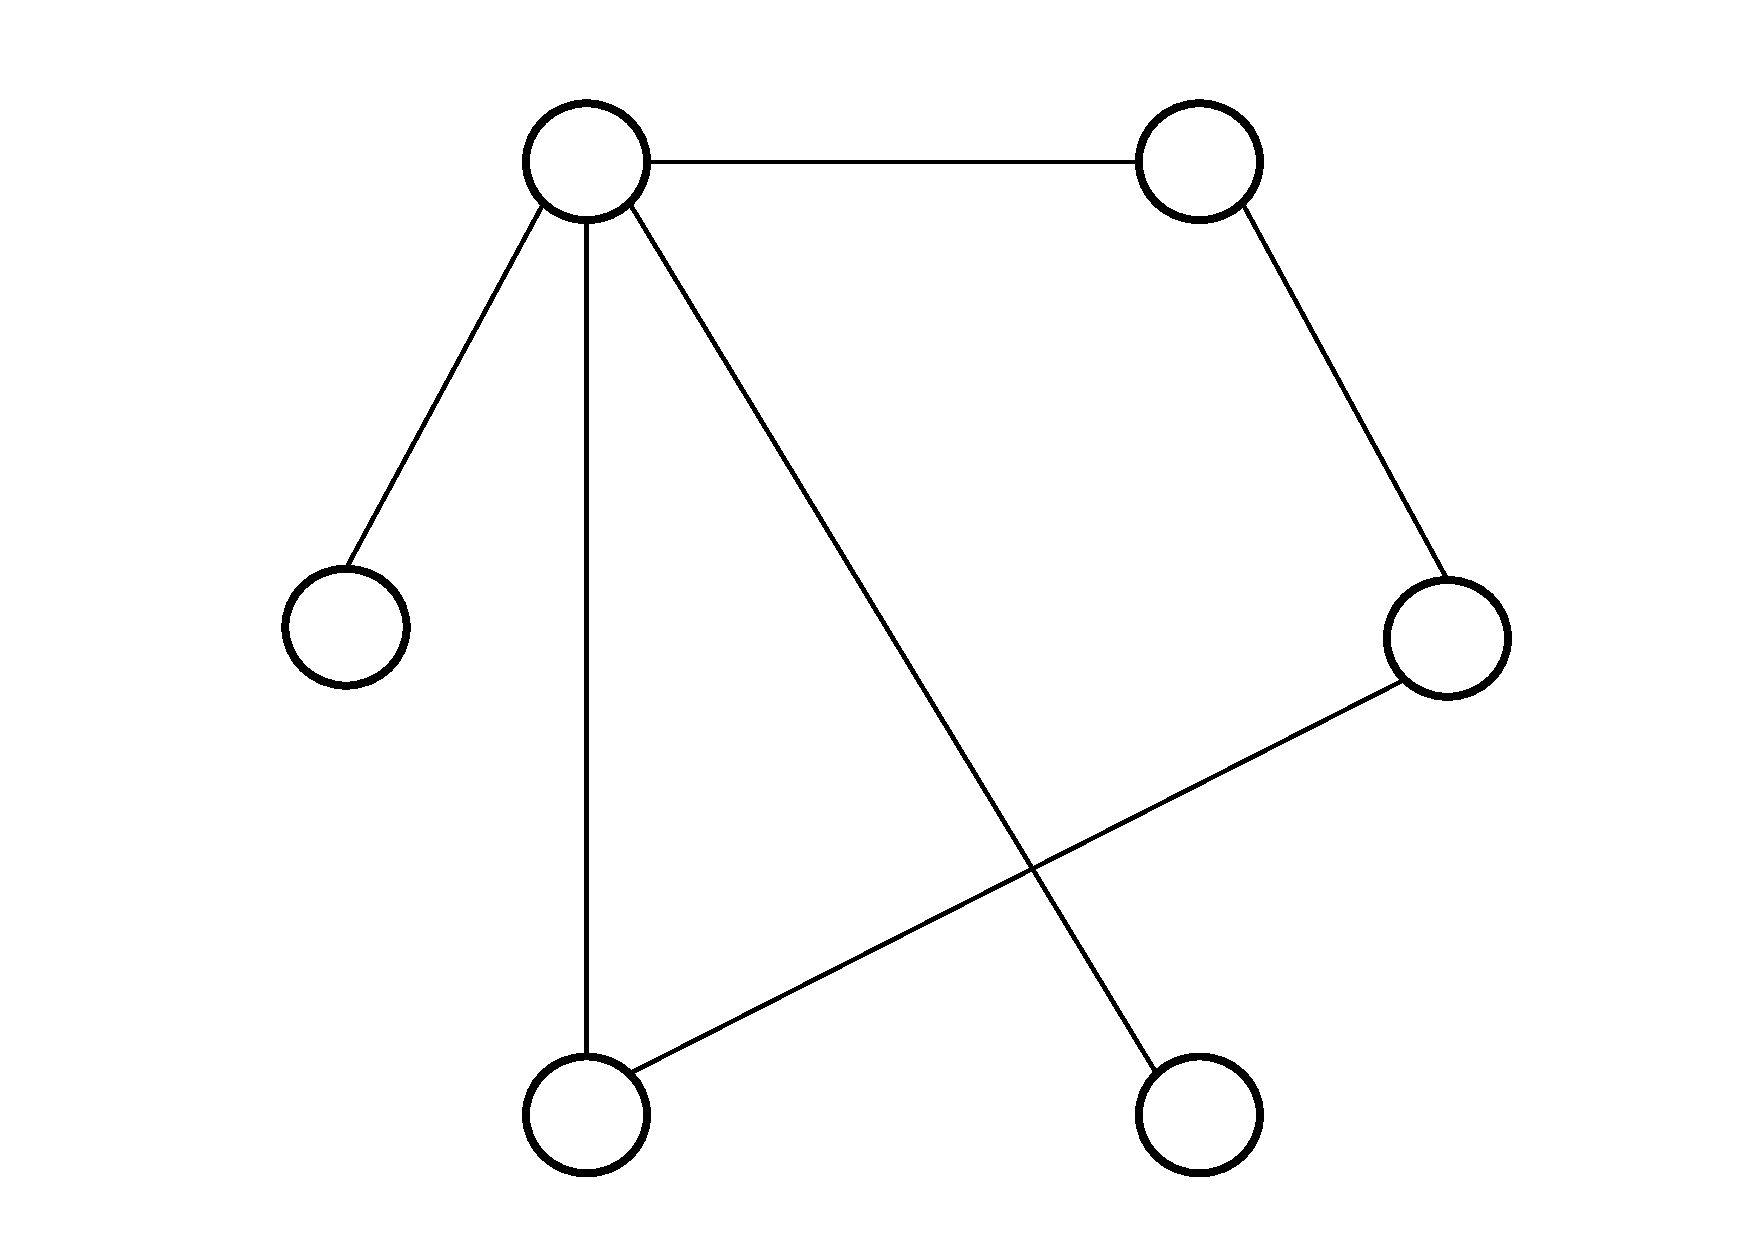
\includegraphics[width=0.3\columnwidth]{chapter2Fig/无向无权重.pdf}}\hfil
	\subfigure[无向有权重网络]{
		\label{2DSF_2} %% label for second subfigure
		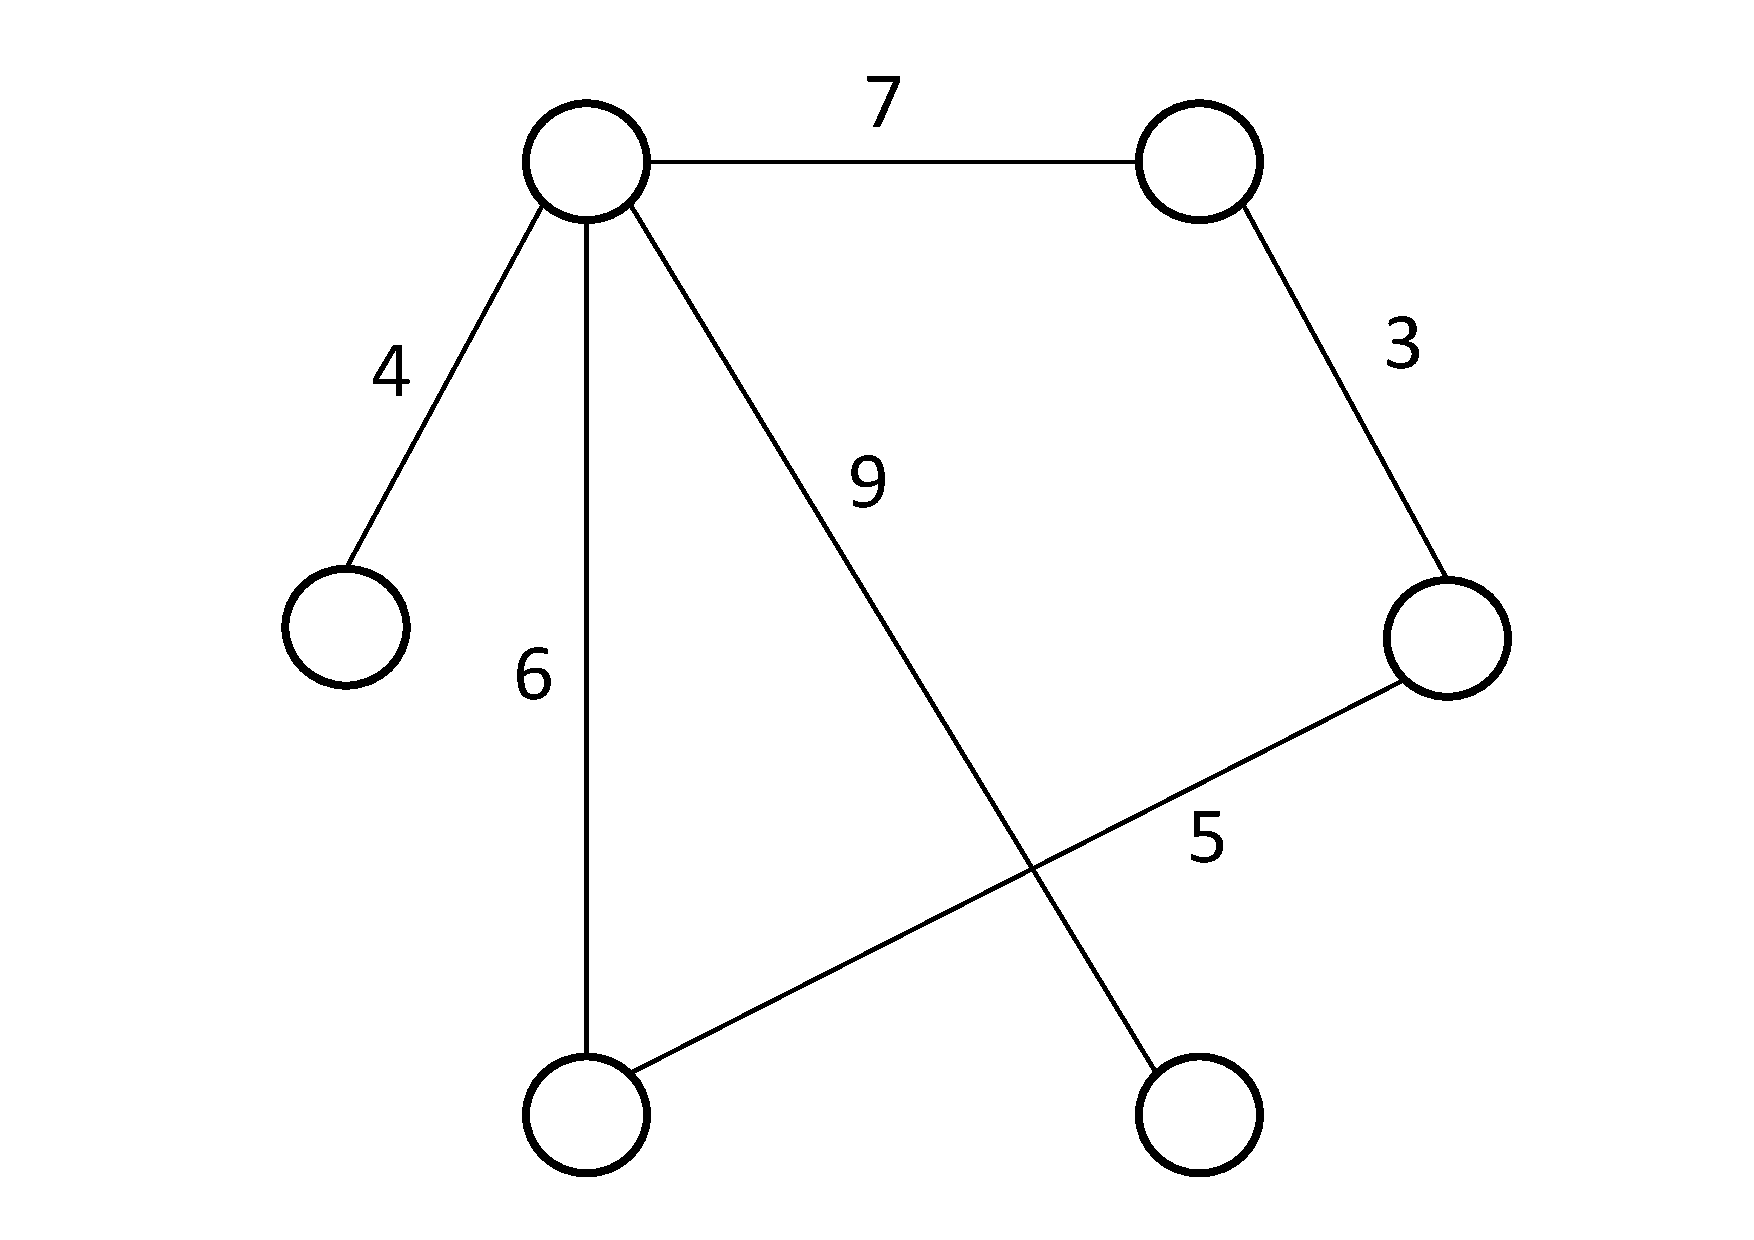
\includegraphics[width=0.3\columnwidth]{chapter2Fig/无向有权重.pdf}}
	
	\subfigure[有向无权重网络]{
		\label{2DSF_3} %% label for first subfigure
		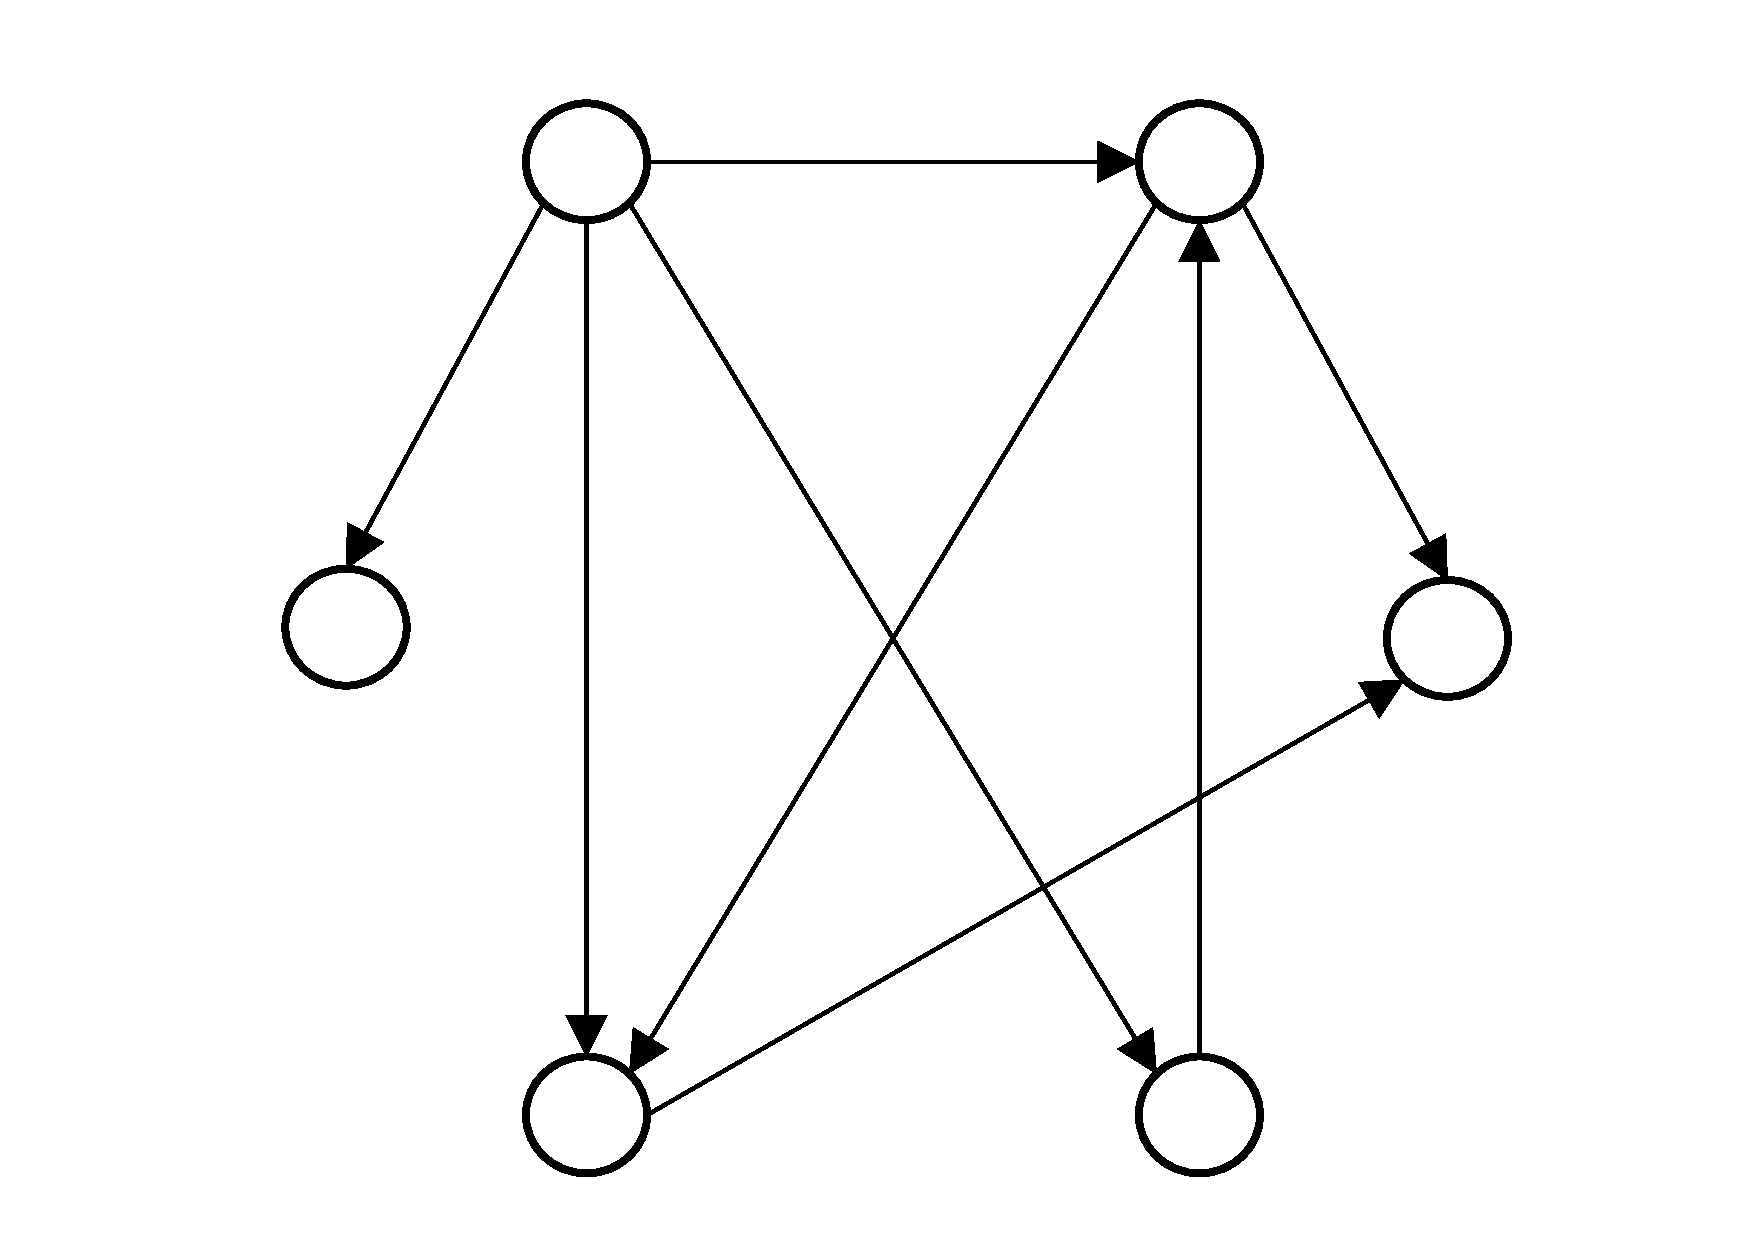
\includegraphics[width=0.3\columnwidth]{chapter2Fig/有向无权重.pdf}}\hfil
	\subfigure[有向有权重网络]{
		\label{2DSF_4} %% label for first subfigure
		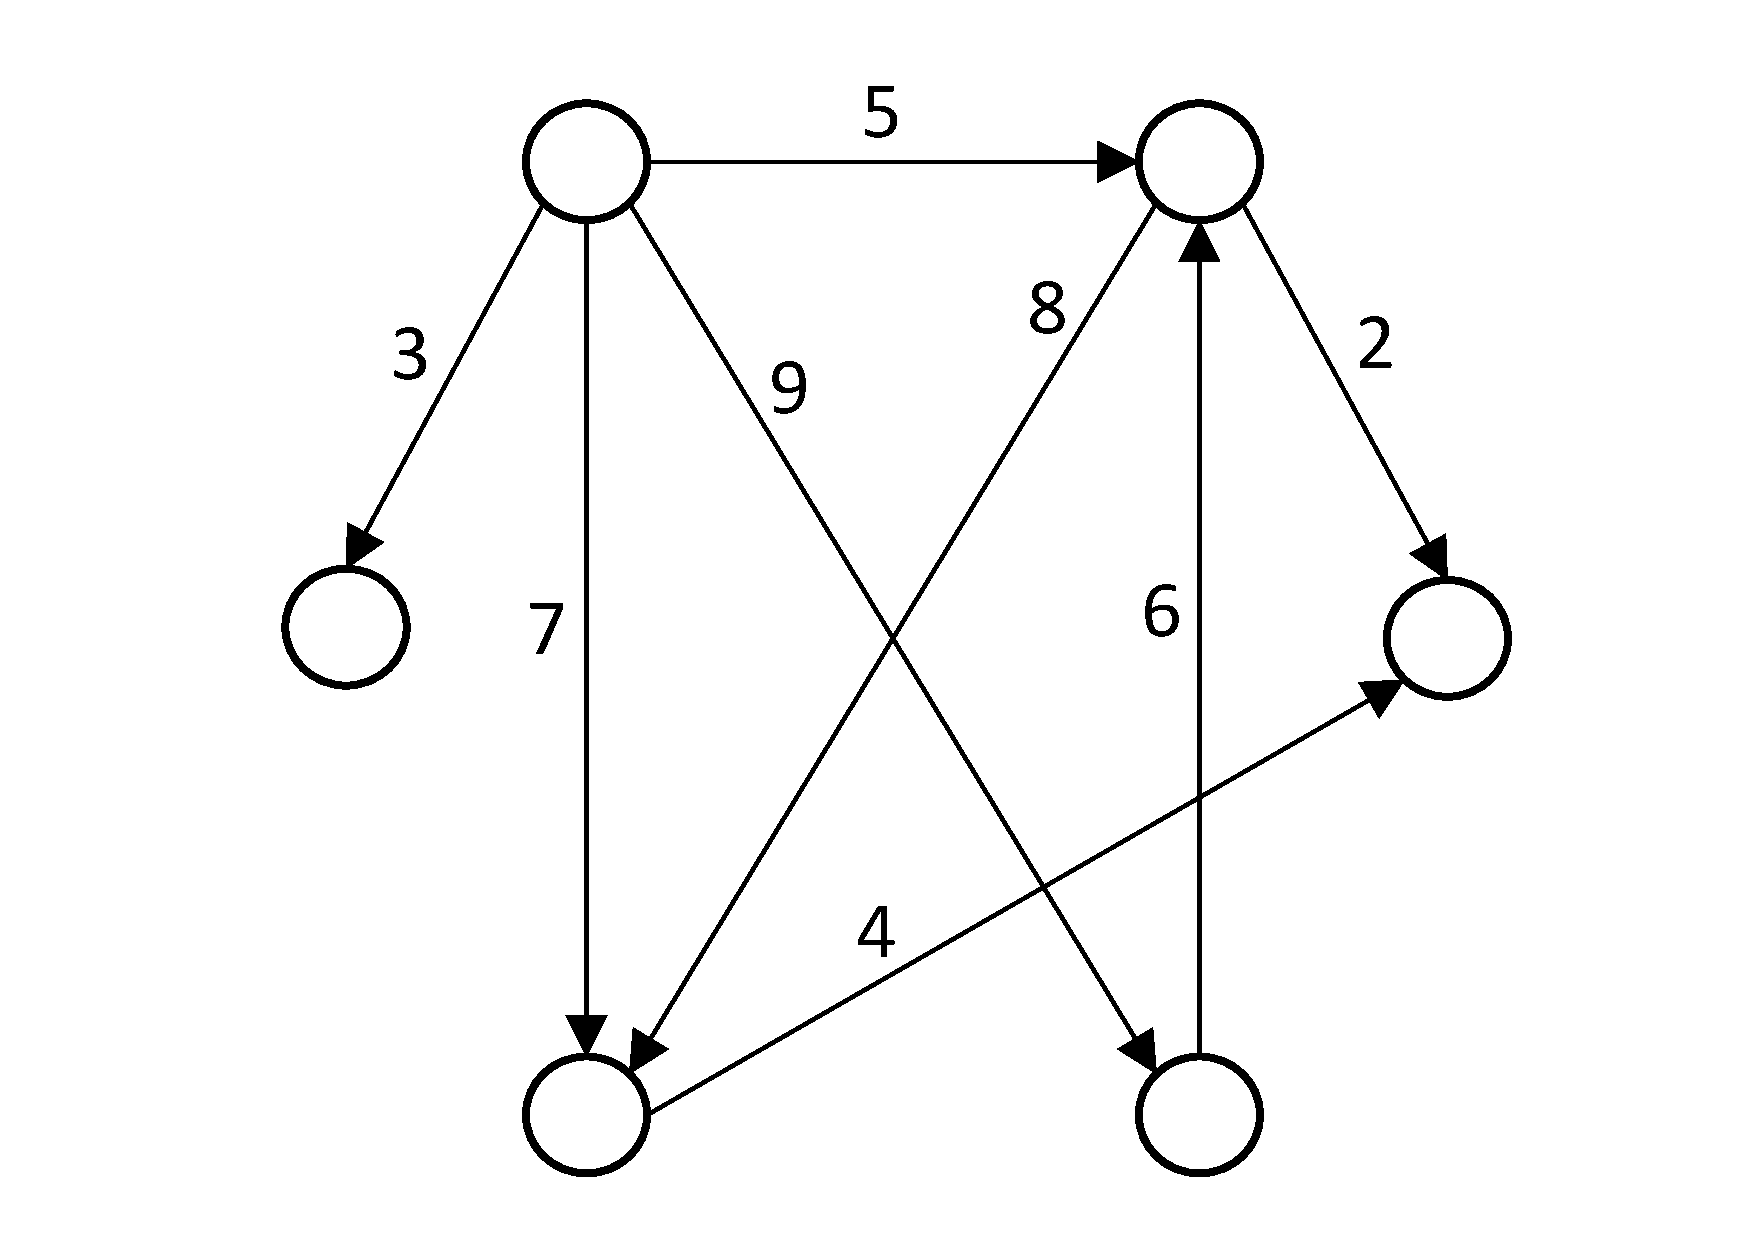
\includegraphics[width=0.3\columnwidth]{chapter2Fig/有向有权重.pdf}}\hfil
	
	\caption{复杂网络图的表示}
	\label{fig2: network} %% label for entire figure
	
\end{figure}

\subsubsection{复杂网络的统计性质}
复杂网络的统计性质主要有:网络的度分布,异质性,同配性,聚类系数,平均最短路径 \cite{汪小帆2006}。

(1) 网络的度分布

对于无向网络而言,一个节点的度,就是节点周围邻居节点的个数。
对于有向网络而言,节点的度分为入度和出度。
特别地,网络的平均度$ <k> $有:
\begin{equation}
<k> = \frac{\sum_{i=1}^{N}{k_i}}{N}.
\end{equation}
其中,$ N $代表网络节点个数,$ k_i $代表节点$ i $的度。

(2) 异质性

网络的异质性描述了节点连接多样性的系数。
网络的异质性越高,代表网络有更多性质不同的节点。
网络的异质性定义为:
\begin{equation}
H = \frac{<k^2>}{<k>^2}.
\end{equation}

(3) 同配性

网络的同配性描述了网络中度相近的节点是否倾向于相互连接的情况。
一般通过皮尔森系数来计算网络的同配系数:
\begin{equation}
r = \frac{M^{-1}\sum_{i}{j_ik_i}-[M^{-1}\sum_{i}\frac{1}{2}{(j_i+k_i)}]^2}{M^{-1}\sum_{i}\frac{1}{2}{(j_i^2+k_i^2)}-[M^{-1}\sum_{i}{\frac{1}{2}(j_i+k_i)}]^2}.
\end{equation}
其中,$ j_i $和$ k_i $分别为第$ i $条边所连节点的度,$ M $为网络边的总数。
若$ r>0 $,代表该网络是同配的,网络中的节点更倾向于连接与之度相近的节点;
若$ r<0 $,代表该网络是异配的,网络中度较大的节点更倾向于连接那些度较小的节点。

(4) 聚类系数

所谓“物以类聚”,我朋友的朋友大概率还是我的朋友,网络的聚类系数描述了这种可能性。
一般而言,网络聚类系数分类为:局部聚类系数和整体聚类系数。在无向图中,单个节点聚类系数定义为:
\begin{equation}
C(i) = \frac{2|\{e_{jk}:v_j,v_k\in L(i), e_{ij}\in E\}|}{k_i(k_i-1)}.
\end{equation}
其中,$ L(i) $代表与节点$ i $相连的所有节点集合,$ k_i $代表节点的度。
换句话说,节点的局部聚类系数等于与它相连的顶点所连边的数量,除以这些顶点可以连出的最大边数。
特别地,网络的平均聚类系数$ <C> $为该网路中所有节点聚类系数的算数平均数。

(5) 平均最短路径

平均最短路径描述了网络节点间的分离程度,定义为:
\begin{equation}
<d> = \frac{\sum_{i=1}^{N}\sum_{j=1}^{N}d(i,j)}{N^2}.
\end{equation}
其中,$ d(i,j) $指的是节点$ i $和节点$ j $的最短路径长度。

\subsubsection{常见网络的模型}
网络的拓扑结构千变万化,在这里简要介绍常见的三种规则网络模型和三种随机网络模型。

(1) 规则网络模型

常见的规则网络模型有:全局耦合网络、最近邻耦合网络、星形网络。
全局耦合网络也称完全图,如图\ref{Fig2:several_network} (a),指的是网络中任意两个节点都存在连接的边。
很明显,全局耦合网络的连边随着节点数量的增加呈线指数增长曲线。
虽然全局耦合网络任意两个节点之间都可以进行信息交流,但在现实生活中,维护这样一个网络所需要的成本太高。
事实上,很多大型网络都是稀疏的,他们边的数量最多是$ O(N) $。
最近邻耦合网络,如图\ref{Fig2:several_network} (b),指的是网络的节点只与其相邻的节点互连,网络整体成为了一个环状。最近邻耦合网络具有高聚类的特性。
星形网络,如图\ref{Fig2:several_network} (c),只有一个节点与其他所有节点相连,不同节点之间的信息交流极大地依赖于中心节点。电话网络中总机和分机的连接采用的就是星形网络。星形网络稳定性较好,易于扩展,但实际操作过程中布线困难,依赖中心节点。如果中心节点收到毁坏,则网络会陷入瘫痪。

\begin{figure}[ht]
	\centering
	\subfigure[全局耦合网络]{
		%%\label{2DSF_1} %% label for first subfigure
		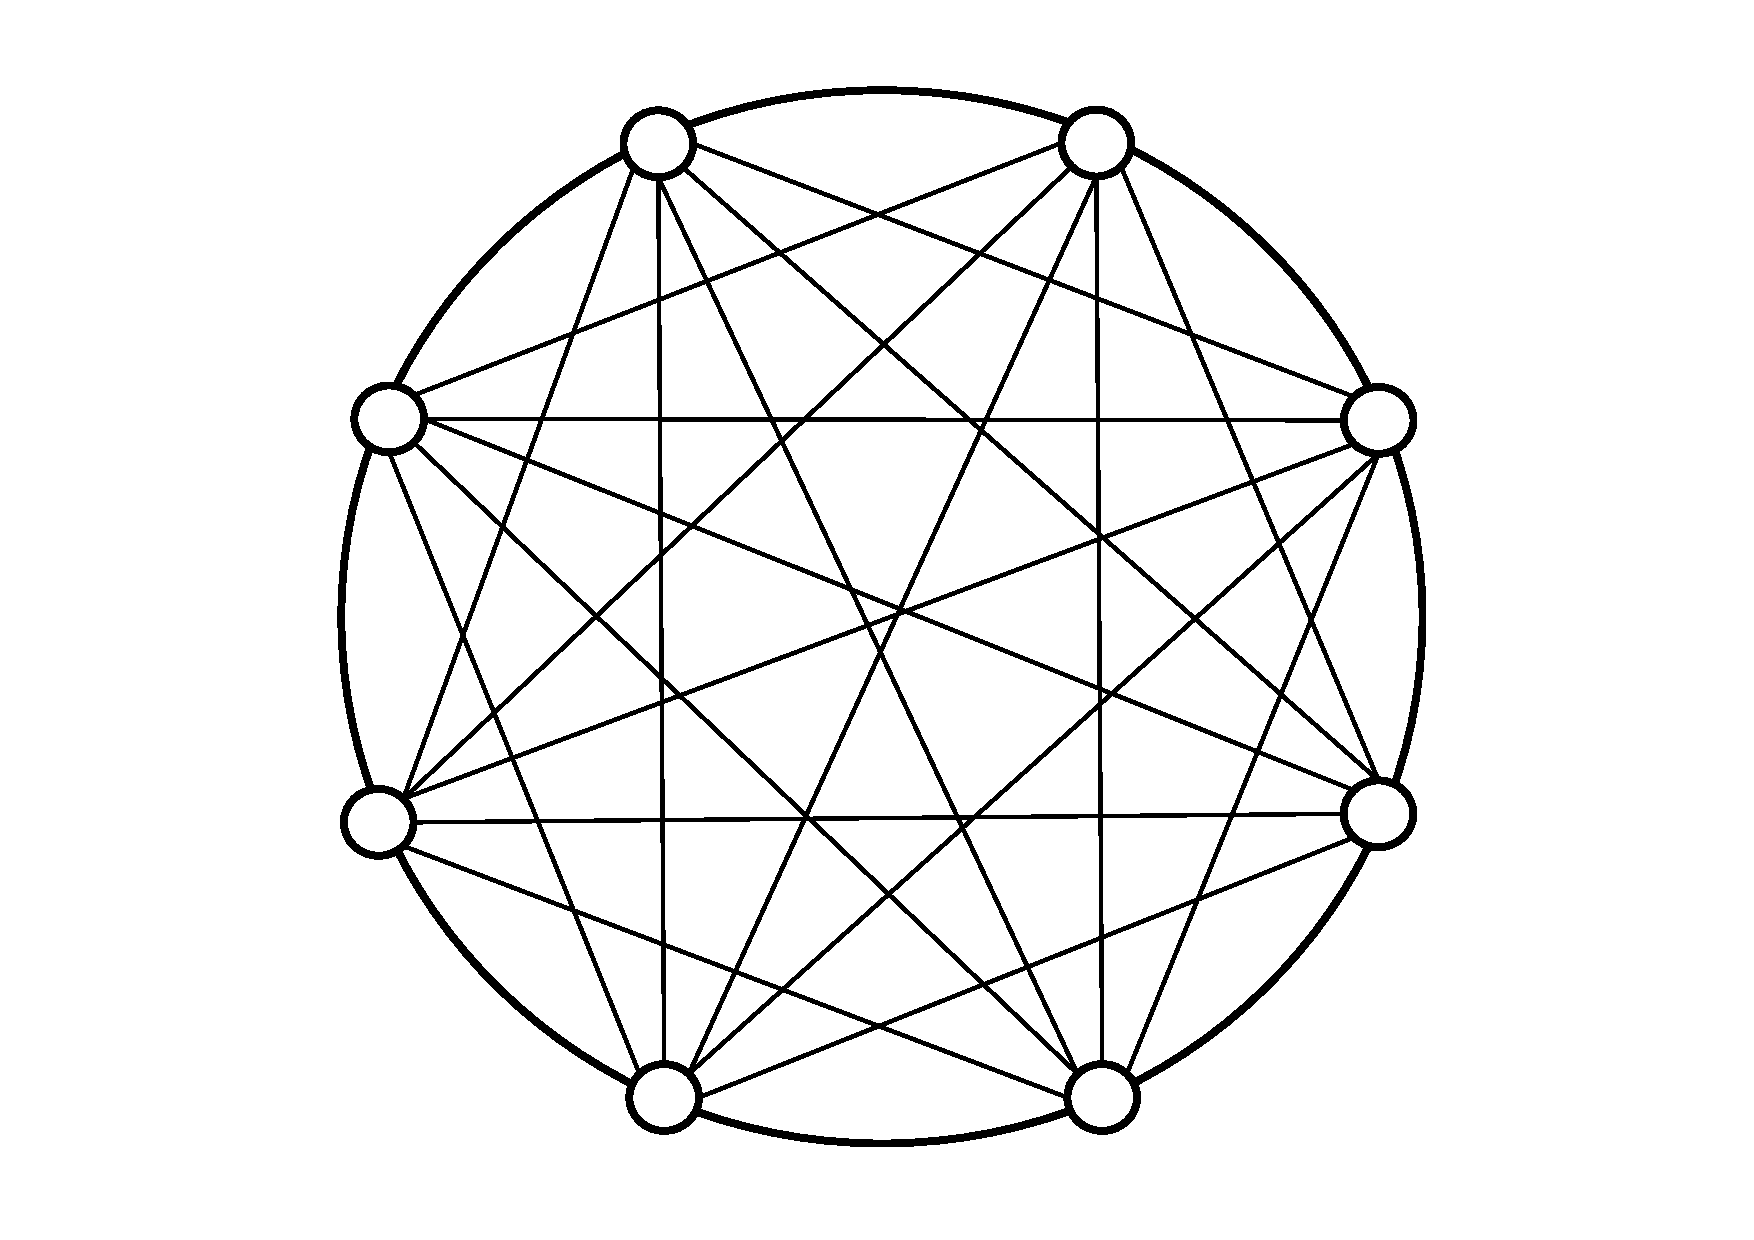
\includegraphics[width=0.3\columnwidth]{chapter2Fig/全局耦合网络.pdf}}\hfil
	\subfigure[最近邻耦合网络]{
		%%\label{2DSF_2} %% label for second subfigure
		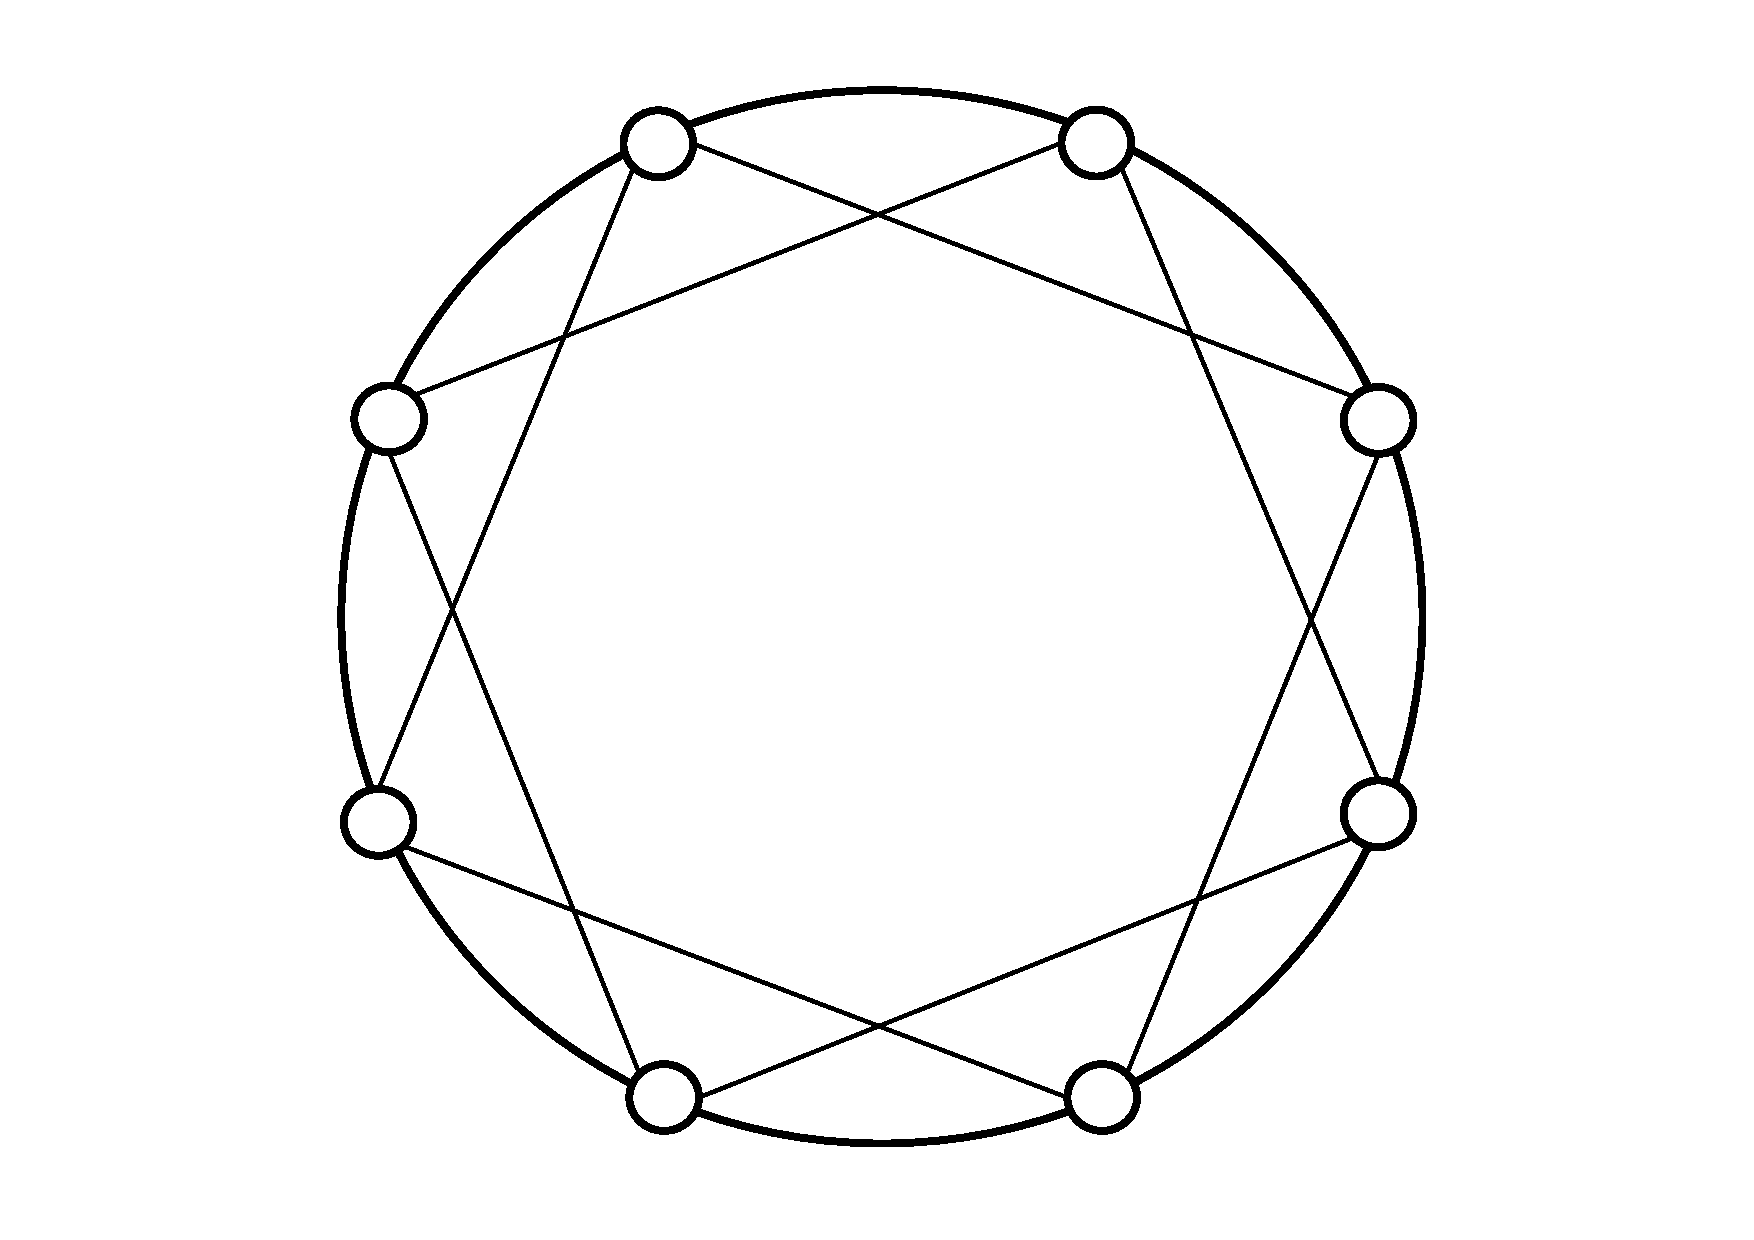
\includegraphics[width=0.3\columnwidth]{chapter2Fig/最近邻耦合网络.pdf}}	
	\subfigure[星形网络]{
		%%\label{2DSF_3} %% label for first subfigure
		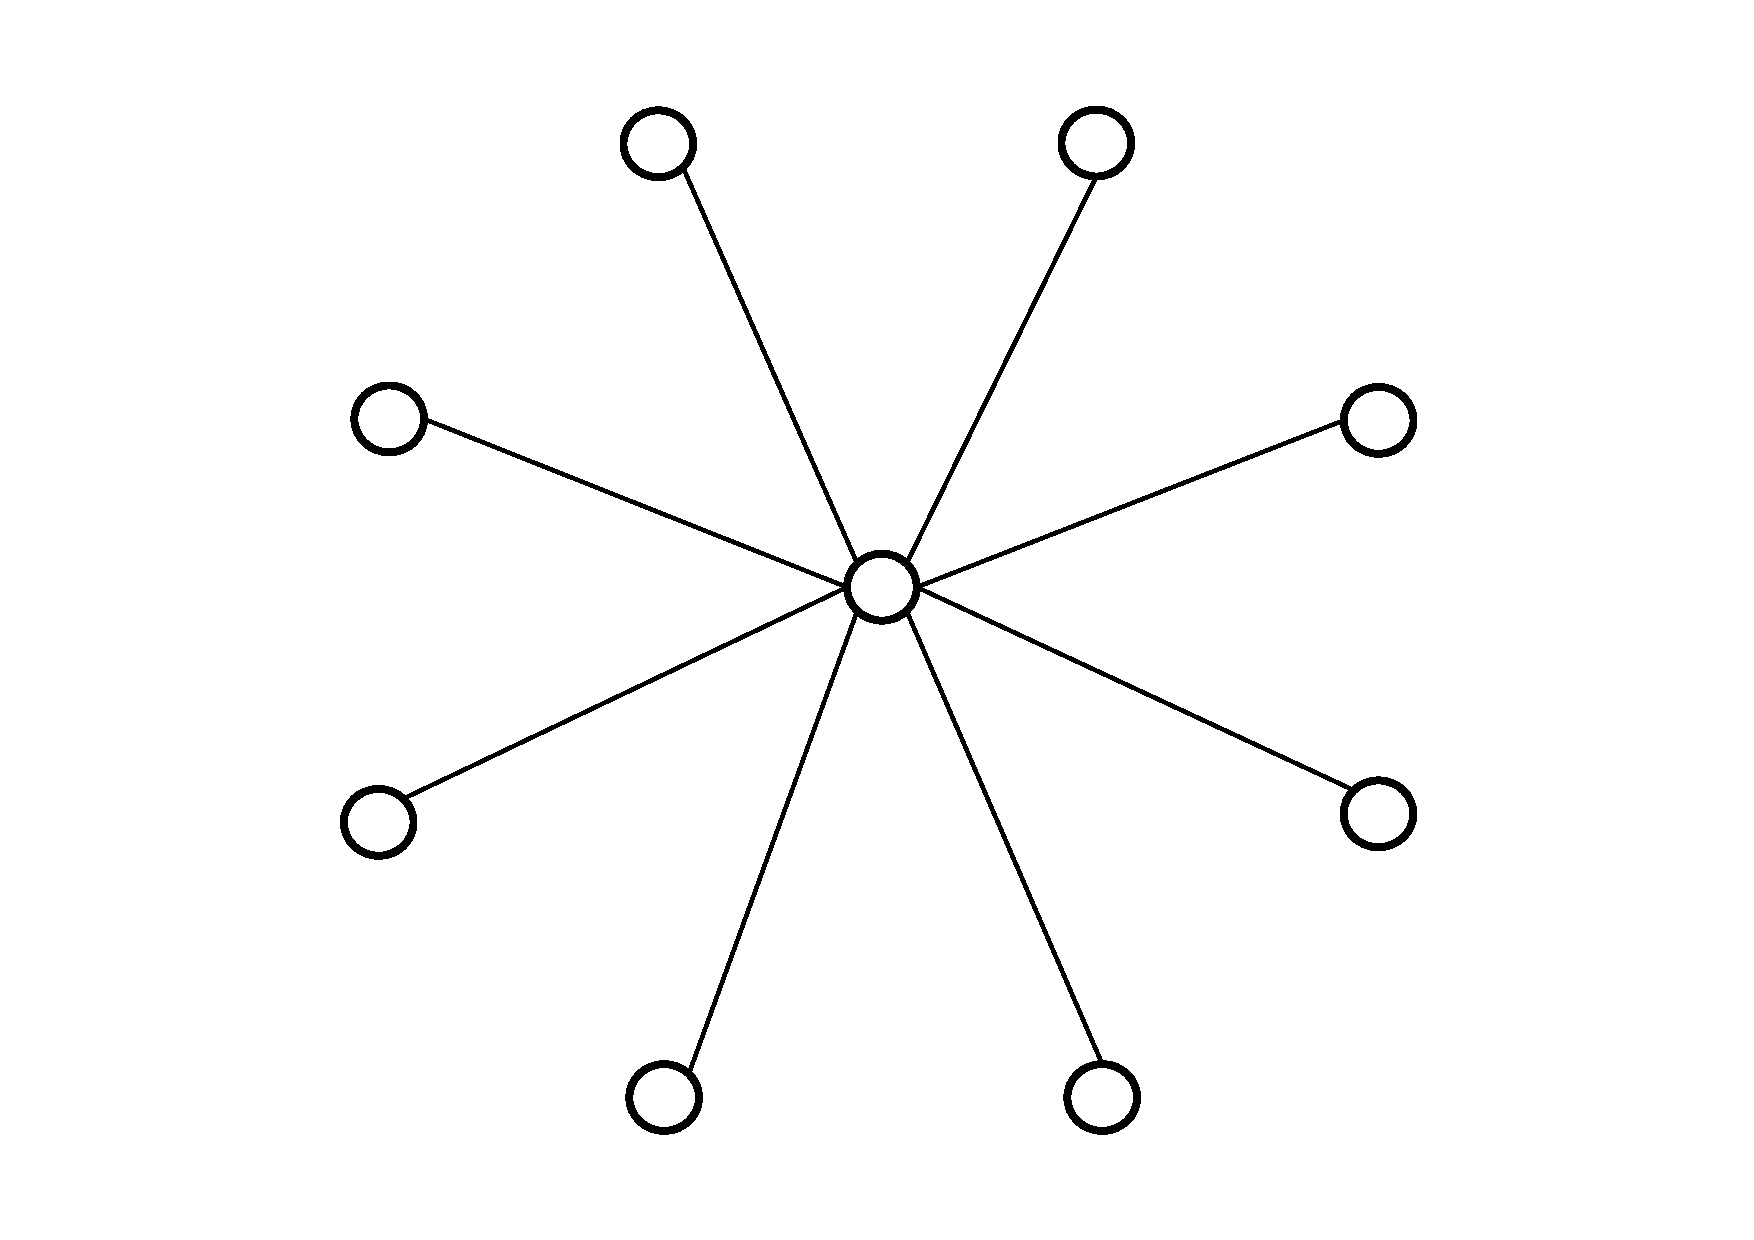
\includegraphics[width=0.3\columnwidth]{chapter2Fig/星形耦合网络.pdf}}\hfil
	
	\caption{几种规则网络}
	\label{Fig2:several_network}
	%\label{figure_2DSF} %% label for entire figure	
\end{figure}




(2) ER(Erd\"{o}s-R{\'e}nyi)随机网络 \cite{Erdoes1959}

ER随机网络又称ER随机图。ER随机图有两种构造方式:
1. $ G(N,p) $,给定$ N $个节点以及节点间的连边概率$ p $,两两节点按照概率$ p $进行连边,直到所有的节点对都被选择;
2. $ G(N,M) $,给定$ N $个节点以及需要添加的边数$ M $,随机选择一组没有进行连边的节点,在他们之间连边,直到所有边数$ M $已被添加完。
如图\ref{Fig: random} (a),该ER随机网络由$ 50 $个节点,节点间连边概率为$ 0.1 $构造而成。

\begin{figure}[t]
	\centering
	\subfigure[ER随机网络]{
		%%\label{2DSF_1} %% label for first subfigure
		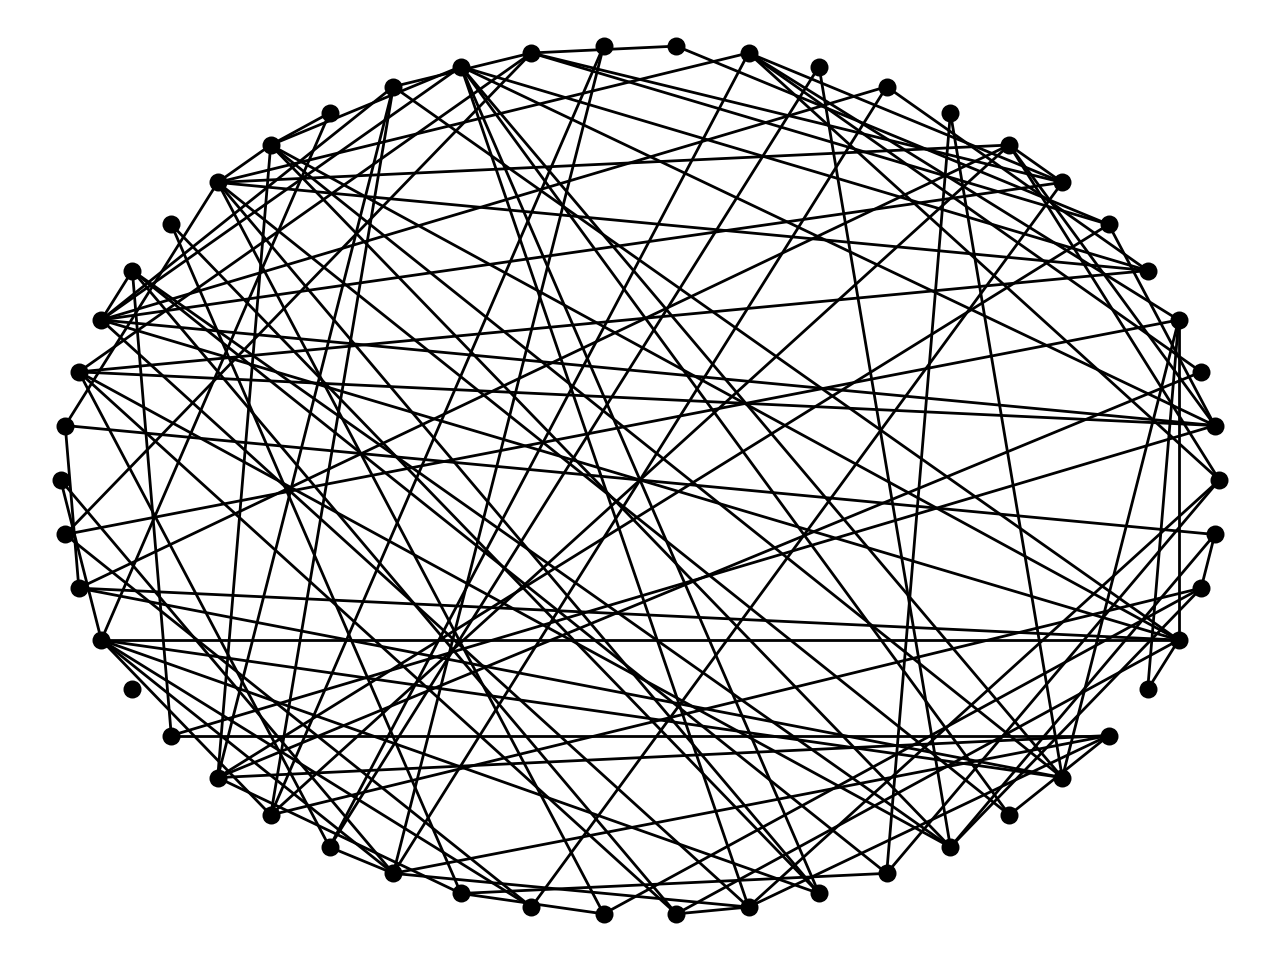
\includegraphics[width=0.3\columnwidth]{chapter2Fig/ER.png}}\hfil
	\subfigure[WS小世界网络]{
		%%\label{2DSF_2} %% label for second subfigure
		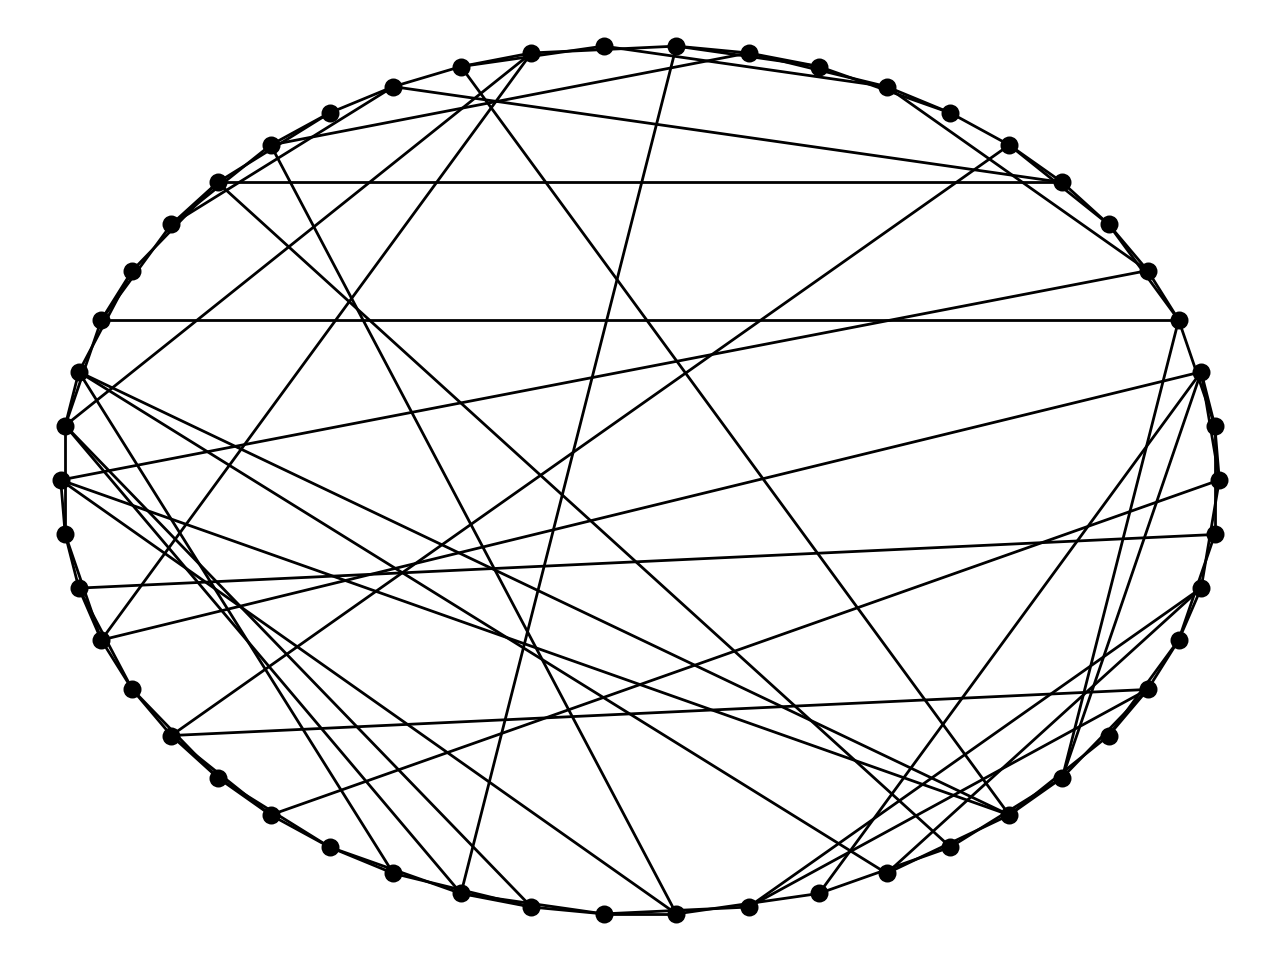
\includegraphics[width=0.3\columnwidth]{chapter2Fig/WS.png}}	
	\subfigure[BA无标度网络]{
		%%\label{2DSF_3} %% label for first subfigure
		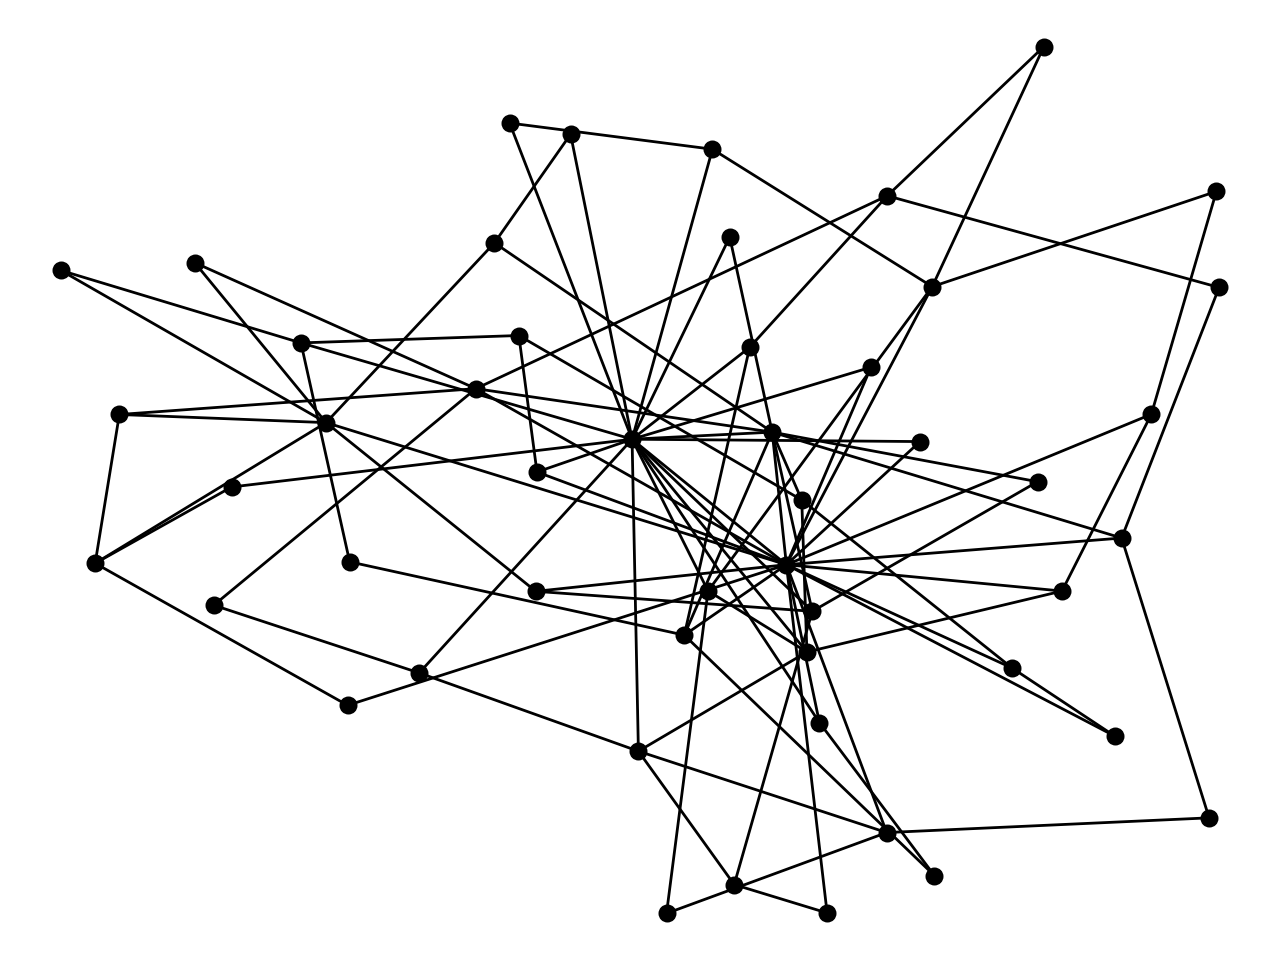
\includegraphics[width=0.3\columnwidth]{chapter2Fig/BA.png}}\hfil
	
	\caption{几种随机网络}
	\label{Fig: random}
	%\label{figure_2DSF} %% label for entire figure	
\end{figure}

(3) WS (Watts和Strogatz) 小世界网络 \cite{Watts1998}

现实中的网络通常具有小世界现象,即:虽然网络中有些节点不具有连边,但任意两个节点之间的最短路径长度远小于节点的数量。
“六度分隔理论”就是对小世界现象的最好阐述,“六度分隔理论”是指,人与陌生人的关系不超过六重,你通过六个人就能够认识世界上任何人。
由于ER随机图无法描述这种小世界这种特性,Watts和Strogatz提出了WS小世界模型算法:
1. 初始网络是有$ N $个节点的最近邻耦合网络,每个节点都和与之左右相邻的$ K/2 $个节点直接相连,$ K $是偶数;
2. 以概率$ p $随机重连初始网络的原有边,重连方式为边的一个节点不变,另一个节点随机选择,且规定在无重边和自环。
如图\ref{Fig: random} (b),该WS小世界网络有$ 50 $个节点,每个节点有$ 4 $个邻居,以概率$ 0.3 $进行重连边。


(4) BA (Barab\'{a}si和Albert) 无标度网络 \cite{Durrett2007}

Barab\'{a}si和Albert发现,在现实生活中,很多网络不同于ER随机图的完全随机,它们的度都近似服从于泊松分布,例如:WWW网络、蛋白质网络、Internet网络等等。
这类网络的度分布在平均值附近有一个峰值,然后服从指数迅速衰减。
于是,他们提出了实际网络中出现的重要特性:
1. 网络的增长。在现实网络中,网络的规模是不断增长的,具体表现为节点数量的增加。例如,在人际关系网络中,人们每天都在认识新的人;
2. 优先连接。网络的规模在扩大的同时,新增的节点更倾向于连接那些已有的高连接度的节点。例如在论文引文网络中,新发表的文章更倾向于引用那些已经被广泛引用的文献。

基于这两个特性,Barab\'{a}si和Albert提出了BA无标度网络算法:
1. 初始网络是一个全局耦合网络,有$ m_0 $个节点,以后每加入一个新节点,则新节点连接$ m $条边到已存在的节点上,且满足$ m<m_0 $;
2. 新节点与已存在节点$ i $连边的概率是:$ \Pi_i={k_i}/ {\sum_{j}{k_j}} $,其中,$ j $为已存在的网络节点,直至节点数量满足要求。
如图\ref{Fig: random} (c),该BA无标度网络有$ 50 $个节点,每次随机加入$ 2 $条连边。

\subsection{同步和控制模型}
网络的控制问题从同步问题而来,而同步问题中最经典的就是Kuramoto相位同步模型。因此,本节从经典的相位同步出发,简单讲解了相位同步,然后关联到一般性的同步过程和网络牵制控制过程。

\subsubsection{Kuramoto同步模型}
一般认为,如果两个耦合的节点的相位$ \theta_i $和$ \theta_j $以一定的比率$ m:n $锁定,并小于某个给定的常数$ \epsilon $,即$ |m\theta_i-n\theta_j|<\epsilon $,则称这两个节点达到了相位同步。相位同步是一种简单的同步,在现实生活中很多应用,如发电机之间的并列运行,导航定位等等。相位同步中,最经典的是Kuramoto同步模型,在这个模型中,每个振子(节点)的动力学方程可以描述成 \cite{Rodrigues2016}:

\begin{equation}
\frac{d\theta_i}{dt}=\omega_i+\frac{c}{N}\sum_{j=1}^{N}(\sin \theta_j-\sin \theta_j), \quad i=1,...,N.
\end{equation}
其中,$ \theta_i $和$ \omega_i $代表第$ i $个的振子的相位和固有频率,$ N $代表整个系统共有$ N $个振子,$ c>0 $为节点之间的耦合强度。


从上述的振子的动力学方程中可以看到,每个振子的相位变化不仅和自身的固有频率$ \omega_i $相关,还与其耦合的节点的相位$ \theta_j $有关。一般认为,在全耦合的振子系统中,耦合强度$ c $足够大时,系统中所有的振子会趋近于同步状态。
如图 \ref{Fig: kuramoto} ,在有20个振子的全耦合网络上模拟了振子同步的过程,耦合强度$ c=1 $,振子震动频率为1赫兹,横纵坐标分别取时间和相位的正弦值。从图中可以很明显地发现,在这个系统中,随着时间的增加,振子的相位趋近于一致,即整个系统是相位同步的。

\begin{figure}[ht]%{.5\linewidth}
	\centering
	% Requires \usepackage{graphicx}
	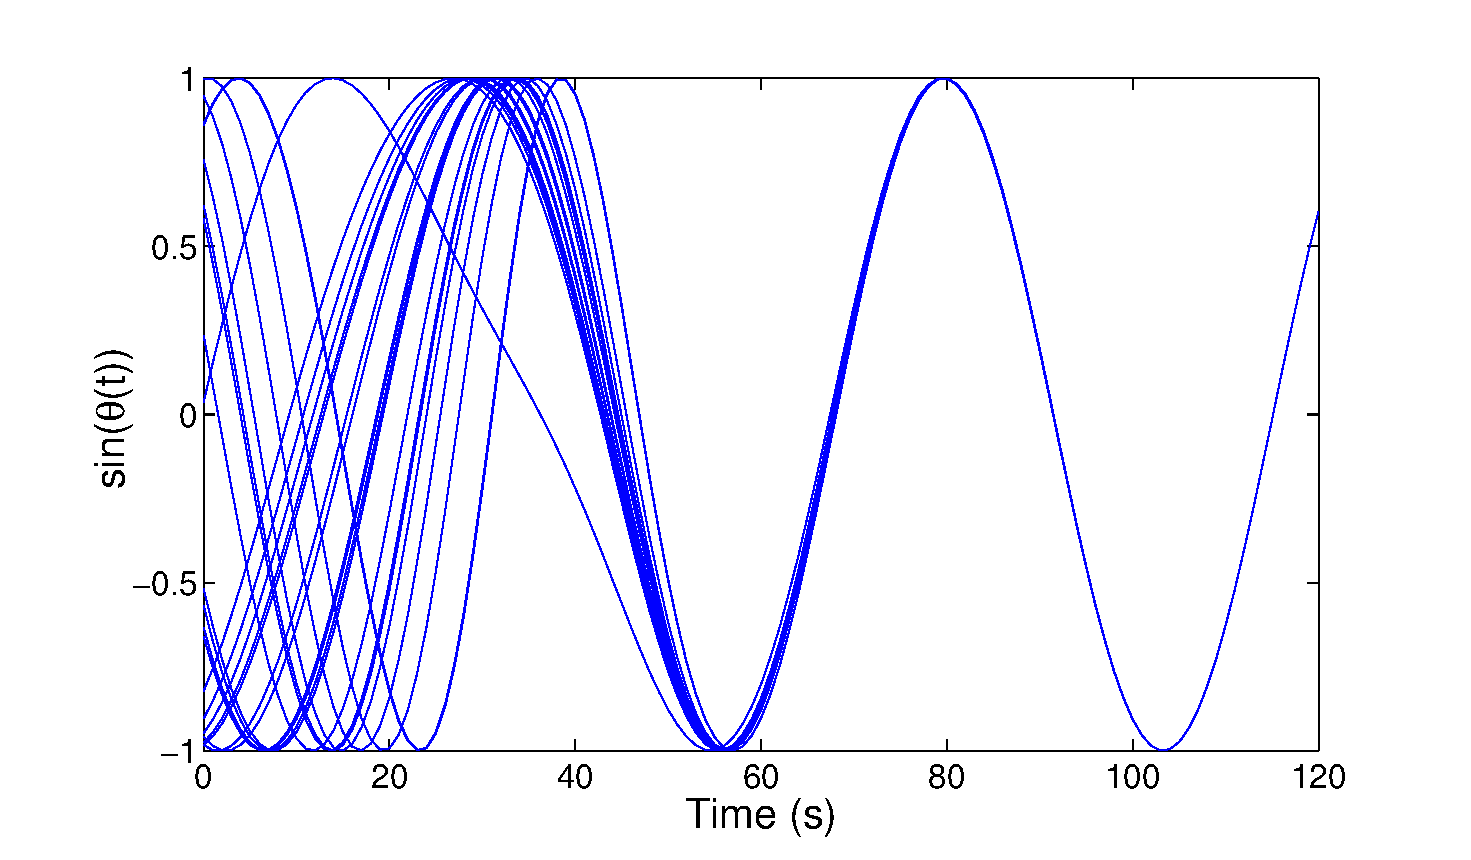
\includegraphics[width=0.9\columnwidth]{chapter2Fig/kuramoto}\\
	% 
	\caption{kuramoto模型振子同步情况}
	\label{Fig: kuramoto}	
	
\end{figure}



\subsubsection{网络同步控制模型}
\label{Sec: control}
现在考虑到一般情况下的同步问题,现给定一个网络$ G = (V, E) $,该网络由$ N=|V| $个节点和$ |E| $条连边构成。
该网络的邻接矩阵可以表示为:$ A=(a_{ij})_{N\times N} $,$a_{ij}=1$ 如果 $(i,j)\in E$,否则$a_{ij}=0$。
那么,该网络的拉普拉斯矩阵有:$ L=(l_{ij})_{N \times N}$,其中, $ l_{ii} $ 为节点$ i $的度,$ l_{ij}=-a_{ij} (i \neq j) $。
另外,网络中每个节点都有状态:$ \textbf{x}_i =(x_{i1},x_{i2},...,x_{in})^T \in R^n, \quad \forall i\in V $。
在连续时间系统中,网络的每个节点的动力学方程可以描述为 \cite{汪小帆2006}:
\begin{equation}
\frac{d\textbf{x}_i}{dt} = f(\textbf{x}_i)-c\sum_{j = 1}^{N}l_{ij}H\textbf{x}_j,\quad \forall i\in V.
\label{Eq: self_dynamics}
\end{equation}

其中,$ f(\textbf{x}_i) $为节点自身的状态改变情况,类似于Kuramoto模型中每个振子的固有频率;$ -c\sum_{j = 1}^{N}l_{ij}H\textbf{x}_j $描述了节点$ i $与其他节点的耦合作用;$ c>0 $ 是耦合强度,描述了节点之间信息交流的强弱;$ H=(h_{ij})_{n \times n} $是一个方阵,描述了节点之间的耦合方式。
和Kuramoto单维的相位同步模型不同,方程\ref{Eq: self_dynamics}描述了网络一般性的同步问题,考虑到了节点$ \textbf{x}_i =(x_{i1},x_{i2},...,x_{in})^T $多个维度的同步情况。

在特殊情况下,网络可能存在自发性同步行为,但在大部分情况下,网络是无法自发性同步的(或同步状态是无法稳定的)。为了使网络达到稳定的同步,可以人为地控制网络中的某些节点,对其施加一个反馈作用。
现记同步稳定状态的平衡点(稳定点):$\overline{\textbf{x}} = (\overline{x}_1, \overline{x}_2, ..., \overline{x}_n)^T$。
为了让网络中的每个节点都达到这种稳定状态,即$x_1(t) = x_2(t) = ... = x_N(t) = \overline{\textbf{x}} $,现对网络的某些节点施加一个反馈作用。假设节点集合$ P $为人为施加的控制节点集合,对于整个网络动力学系统有 \cite{Zhou2019}:
\begin{equation}
\left\{
\begin{aligned}
&\frac{d\textbf{x}_i}{dt} = f(\textbf{x}_i)-c\sum_{j = 1}^{N}l_{ij}H\textbf{x}_j,\quad  i \notin P, \\
&\frac{d\textbf{x}_{i}}{dt} = f(\textbf{x}_{i})-c\sum_{j = 1}^{N}l_{ij}H \textbf{x}_j-cdH(\textbf{x}_{i}-\overline{\textbf{x}}), \quad i\in P.
\end{aligned}
\right.
\label{Eq:all_dynamical}
\end{equation}
其中,$ f(x) $为节点自身状态变化函数,对于稳定点也满足$\frac{d\overline{\textbf{x}}}{dt}=f(\overline{\textbf{x}})$;$ d>0 $代表控制节点的反馈强度。
在网络牵制控制过程中,动力学方程\ref{Eq:all_dynamical}描述了控制节点和普通节点的状态变化过程。从方程可以看到,控制节点通过一个负反馈作用,来调节节点状态加速度的改变,进而引起节点状态的变化;若控制节点的状态大于平衡点($ x_i>\textbf{x}$),则该节点加速度变小,控制节点倾向于“慢下脚步”,等待其他节点;若控制节点的状态小于平衡点($ x_i<\textbf{x} $),则该节点加速度增大,控制节点则“加快脚步”,跟上其他节点的状态。

通过控制节点的负反馈作用,网络也就更容易受到控制,到达同步稳定的状态。然而,最佳控制节点的选择是一个NP-hard问题。因此,为了找到效果最好的牵制控制节点,在本章后续部分,介绍了几种经典的重要节点检测算法。

\subsection{重要节点检测算法}
本节主要介绍了几种经典的重要节点检测算法,包括:度中心性算法,介数中心性算法,接近中心性算法,特征向量中心性算法,PageRank算法,K-shell分解算法和ESI方法。


(1) 度中心性(Degree centrality) \cite{Brodka2011}

以社交网络(微信)为例,一般认为微信好友越多,社交圈子越广,该微信用户也就更为重要,这就是节点度中心性。
无向图的度中心性定义为:
\begin{equation}
DC_i = \frac{k_i}{N-1}.
\end{equation}
很明显,度中心性只与节点的度有关,是网络的一个局部特征。
对于有向图来说,还应考虑到节点的出度和入度。

(2) 介数中心性(Betweenness centrality) \cite{Newman2005}

节点介数中心性指的是节点在其他两个节点最短距离间充当中介的次数。
节点的介数中心性定义为:
\begin{equation}
BC_i = \sum_{i\neq j \neq k}\frac{n_{jk}^i}{g_{jk}}.
\end{equation}
其中,$ g_{jk} $代表节点$ j $和节点$ k $最短路径的条数,$ n_{jk}^i $代表节点$ j $和节点$ k $最短路径经过节点$ i $的次数。
节点的介数中心性越大,代表该节点充当网络中其他节点信息交流的中介次数越多,也就意味着该节点更为重要。

(3) 接近中心性(Closeness centrality) \cite{Okamoto2008}

节点的接近中心性指的是该节点到其他所有节点的最短距离总和的倒数。
无向图的接近中心性定义为:
\begin{equation}
CC_i = \frac{1}{\sum_{j}^{N}d{(i,j)}}.
\end{equation}
其中,$ d(i,j) $指的是节点$ i $到节点$ j $的最短距离。
一般而言,节点接近中心性越高,代表这个节点距离其他节点也越近,节点在空间上也处于比较中间的位置,节点也就更加重要。
对于有向图来说,接近中心性还分为入接近中心性和出接近中心性,分别对应着物理上节点的“整合力”和“辐射力”。

(4) 特征向量中心(eigenvector centrality) \cite{Perra2008}

节点的特征向量中心性认为,某个节点重要性不仅和该节点有关,还与该节点相连的邻居节点有关。
特征向量中心性定义为:
\begin{equation}
EC_i =  c\sum_{j=1}^{N}a_{ij}x_j.
\end{equation}
其中,$ c $是比例常数,$ a_{ij} $代表网络邻接矩阵的元素,$ x_j $代表邻接矩阵和特征值$ c^{-1} $对应的特征向量的元素。

(5) PageRank算法 \cite{Page1999}

谷歌搜索引擎的网页重要性排序采用的就是PageRank算法。
对于网页$ u $而言,该网页的PageRank指标定义为:
\begin{equation}
R(u) = \beta \sum_{v\in B_u}{\frac{R{(v)}}{|B_u|}}.
\end{equation}
其中,$ \beta $是一个归一化常数,$ v $是一个网页,$ B_u $时节点$ u $相邻网页的集合。
对于一个网络来说,节点的PageRank指标越大,也就意味着在随机浏览时,这个节点更大概率被访问到,这个节点也就更加重要。

(6) K-shell分解算法 \cite{Ma1991}

Kitsak等人认为在只有一个传播源的情况下,节点的度和介数并不能精确描述网络节点的传播能力,因而提出了K-shell分解算法。
K-shell分解算法会递归地剥离网络中度数小于或者等于$ k $的节点,
算法流程为:

1)查找网络中所有度为1 $(k = 1) $的节点,将其节点和连边去掉;

2)经过步骤1)后,残余网络中可能会存在度为1的节点;继续重复步骤1),直至网络中不出现度为1的节点,被删除的节点K-shell值定为1;

3)去除度值小于等于2 $ (k<=2) $的节点及其连边,并在残余网络中重复删除操作,被删除的节点K-shell值定为2;

4)依此类推,直至网络上的所有节点都被赋予K-shell值。

该算法实现简单,适用于大型网络,在疾病传播模型中能够很好的找到最有影响力的节点。但在BA无标度网络和树状网络中表现较差,因为在这两个网络中,大部分节点的K-shell值相近,无法区分差异。

(7) ESI方法 \cite{Amani2017}

Amani等人在研究最佳的网络牵制控制节点集合时,提出了一个近似计算节点最大影响力的ESI方法。该方法基于网络拉普拉斯矩阵的谱分析,通过删除节点后观察网络牵制控制传统判据的扰动情况,对节点的脆弱性进行排序。对于一个节点$ i $ 而言,其ESI指数为:
\begin{equation}
ESI(i) = (X_N^i)^2.
\end{equation}
其中,$ X_N $代表了网络拉普拉斯矩阵最大特征值相对应的特征向量,$ X_N^2 $代表特征向量$ X_N $的第$ i $个元素。


\subsection{评价指标}
在本节中,介绍了两个评价指标:节点重叠指数和皮尔森系数。
在第三章和第四章中,节点重叠指数用来比较控制节点之间的差异;在第四章中,皮尔森系数用来比较传统判据和耦合强度范围的相关性。

(1)节点重叠指数HDI(hub depressed index)\cite{Lue2011}

节点重叠指数衡量了节点集合的重叠比例,对于节点集合$ S_1 $与$ S_2 $,节点重叠指数定义为:
\begin{equation}
{\rm HDI}_{S_1\sim S_2} = \frac{|S_1 \cap S_2|}{max(|S_1|,|S_2|)}.
\end{equation}
明显,$ {\rm HDI}_{S_1\sim S_2}\in [0,1] $。$ {\rm HDI}_{S_1 \sim S_2}\rightarrow 0 $代表集合$ S_1 $与$ S_2 $重叠节点越少;$ {\rm HDI}_{S_1\sim S_2}\rightarrow 1 $代表集合重叠节点越多。

(2)皮尔森系数 \cite{LeeRodgers1988}

皮尔森系数衡量了两个变量的相关性,对于变量$ X $与$ Y $,其皮尔森系数定义为:
\begin{equation}
r_{x,y} = \frac{cov(X,Y)}{\rho_X \rho_Y} = \frac{E[(X-E(X))(Y-E(Y)]}{\rho_X \rho_Y}.
\end{equation}
其中,$ cov(X,Y) $代表了变量$ X $与$ Y $的协方差,$ \rho_X $与$ \rho_Y $代表了变量的标准差,$ E(X) $与$ E(Y) $代表了变量$ X $与$ Y $的期望。
此外,$ r_{x,y}\in[-1,1] $。$ r_{x,y}\rightarrow1 $代表变量$ X $与$ Y $趋近于正相关关系;$ r_{x,y}\rightarrow-1 $代表变量$ X $与$ Y $趋近于负相关关系。


\subsection{本章小结}

本章主要介绍了网络科学基础理论,涵盖了复杂网络的主要性质、网络的同步和控制模型、重要节点检测算法等三大内容。


\clearpage

\section{网络的牵制控制研究}

本章从牵制控制的动力学模型出发,引出衡量网络控制能力的经典比率判据。因为传统比率判据无法精确衡量网络的牵制控制能力,本章提出耦合强度范围和收敛速度两个指标。
这两个指标由作者原创提出,前者决定了网络牵制控制时模型中耦合强度的大小,后者则从李雅普诺夫指数方面,给出了网络控制速度。
耦合强度范围和收敛速度完全不同,他们分别从不同角度刻画了网络牵制控制。
另外,实验还发现传统判据、耦合强度范围和收敛速度这三个指标无法同时到达最优状态。

\subsection{网络的牵制控制}
\subsubsection{稳定性分析}

在章节\ref{Sec: control} 中,动力学方程\ref{Eq:all_dynamical} 描述了牵制控制中控制节点和普通节点的动力学演化过程。
另外,网络也是一个混沌系统,混沌系统的特点是对初值极为敏感,两个极为接近的初始值随时间的变化,其产生的轨道会按照指数幂进行分离,通常用李雅普诺夫指数这个参数来描述这种现象 \cite{Wolf1985}。
为了使节点最终到达的状态得到稳定,现在从结果出发,考虑把网络控制在一个平衡点$\overline{\textbf{x}} = (\overline{x}_1, \overline{x}_2, ..., \overline{x}_n)^T$,则方程\ref{Eq:all_dynamical} 可转化为 \cite{汪小帆2006}:
\begin{equation}
\dot{\xi}_i = [Df+c{\lambda}_iH]{\xi}_i,\quad i=1,2,..,N
\label{Eq: Reduce_MSF}.
\end{equation}
其中,$ Df $代表节点自身演化函数$ f $的雅可比矩阵,$ \xi_i $代表节点状态$x_i$转化后的状态变量,$ {\lambda}_i $代表牵制控制矩阵$ C $ 的特征值,且有$ 0 > {\lambda}_1 \geq {\lambda}_2 \geq ... \geq {\lambda}_N$。$ C=-L-D $,$ D $ 为对角阵 $ D=diag\{d_1,d_2,...,d_N\} $。其中,如果节点$ i $是一个控制节点,则 $ d_i=d $,否则,$ d_i=0 $。牵制控制矩阵$ C $可描述为:
\begin{equation}
C=
\left[
\begin{matrix}
-l_{11}-d_1      & -l_{12}       & \cdots & -l_{1N}       \\
-l_{21}       & -l_{22} -d_2      & \cdots & -l_{2N}      \\
\vdots & \vdots & \ddots & \vdots \\
-l_{N1}       & -l_{N2}       & \cdots & -l_{NN}-d_N       \\
\end{matrix}
\right].
\label{Eq: C}
\end{equation}

考虑式子\ref{Eq: Reduce_MSF}的广义函数,可以得到主稳定方程 \cite{Sorrentino2007}:
\begin{equation}
\dot{y} = [Df + \alpha H]y.
\label{Eq: MSF}
\end{equation}
该方程的最大李雅普诺夫指数$ L_{max} $是关于实数变量$ \alpha $的函数。假设实数变量$ \alpha \in (\alpha_2, \alpha_1) $,由式子\ref{Eq: Reduce_MSF} ,有$ \alpha_2 <c\lambda_i<\alpha_1 $。

在控制理论中,雅普诺夫指数也是衡量系统能否稳定的重要指标。一个混沌系统的最大李雅普诺夫指数大于$ 0 $,代表这个系统中,无论两个轨道的初始间距多么微小,这两个轨道终会随时间而呈指数发散而无法观测。
反之,若一个系统的最大李雅普诺夫指数小于$ 0 $,则这个系统某初始状态可能会收敛,即两个不同的轨道可能会随时间而发生重叠。
因此要使得整个系统稳定,最大李雅普诺夫指数$ L_{max} $必须小于0,即:
\begin{equation}
\Lambda_{max}[Df + \alpha H]<0.
\label{Eq:princple_eigenvalue}
\end{equation}
其中,$ \Lambda_{max} $ 为$ [Df + \alpha H] $的最大特征值。

本节分析了平衡点的局部稳定状态,通过最大李雅普诺夫指数是否小于$ 0 $,来判断平衡点是否能稳定。平衡点能稳定,代表网络有机会得到控制。
因此,最大李雅普诺夫指数小于$ 0 $是网络受控的必要非充分条件。网络得到控制,则该系统的最大李雅普诺夫指数小于$ 0 $;但是,最大李雅普诺夫指数小于$ 0 $不一定意味着网络能够得到控制。
就目前而言,采用李雅普诺夫指数是计算复杂网络牵制控制的最佳方法。


\subsubsection{经典比率判据}
根据主稳定方程\ref{Eq: MSF},最大李雅普诺夫指数是关于实数变量$ \alpha $的函数。
因此通过$ \alpha $的取值范围,网络的牵制控制可以分为三个方面来考虑 \cite{汪小帆2006}:

(1) $ \alpha \in S1 = (-\infty,\alpha_2) $,且 $ \alpha_2 $是一个负实数。
在这种情况下,为了确保控制的稳定状态,只需要有:
\begin{equation}
c\lambda_1<\alpha_2.
\end{equation}
此时,节点对网络的控制强度由$ \lambda_1 $来决定。$ \lambda_1 $越小,耦合强度$ c $的取值范围也就越大,网络也就更容易达到受到控制。

(2) $ \alpha \in S2 = (\alpha_2, \alpha_1) $,且 $ \alpha_2<\alpha_1<0 $。
在这种情况下,为了控制确保稳定状态,耦合强度需要满足不等式:
\begin{equation}
\alpha_2<c\lambda_N,
c\lambda_1<\alpha_1.
\label{Eq: coupling_strength}
\end{equation}
在耦合强度满足以上关系时,该网络的受控状态是渐进稳定的。
通常而言,公式\ref{Eq: coupling_strength}被当作网络牵制控制比例判据,并定义:
\begin{equation}
R = \frac{\lambda_1}{\lambda_N} > \frac{\alpha_1}{\alpha_2}.
\label{Eq: R}
\end{equation}
$ R $称之为经典比率判据,其只与网络自身的拓扑结构和控制节点有关。
$ R $值越大,代表节点对网络的控制能力也就越强。

(3) $ S3 = \emptyset $。在这种情况下,网络无法得到控制。在本文中,不考虑这种情况。

\subsection{耦合强度范围与收敛速度}
事实上,经典比率判据$ R $无法精确衡量节点对网络的牵制控制能力,在极端情况下,$ R $会失效。因此,本节针对于网络牵制控制问题,将节点对网络的牵制控制能力可以分为两个部分:耦合强度范围和网络的收敛速度。
耦合强度范围由比例判据而来,指明了要使网络得到控制,耦合强度需要满足的条件;
收敛速度即网络受控稳定的速度,其与主稳定方程的最大李雅普诺夫指数有关。
耦合强度范围和收敛速度由作者原创,这两者分别从不同角度刻画了网络牵制控制的情况,关联性极低。

\subsubsection{耦合强度范围}
为了控制一个网络,使之到达稳定的状态,耦合强度必须满足公式 \ref{Eq: coupling_strength} 。因此,耦合强度范围定义为:
\begin{equation}
\omega = \frac{\alpha_2}{\lambda_N} - \frac{\alpha_1}{\lambda_1} >0.
\label{Eq: omega}
\end{equation}
很明显,耦合强度范围为耦合强度满足控制条件的差值。
节点之间耦合强度可供选择的范围越大,也就更容易找到一个合适的耦合强度的值来促使网络到达受控稳定状态。
因此,同经典判据一样,耦合强度范围也越大越好。
为了使耦合强度范围更大,研究人员可以采用不同的重要节点检测算法,来获取网络的牵制控制节点。

需要注意到的是,经典判据$ R $和耦合强度$ \omega $是两个完全不同的衡量标准。
经典判据$ R $只依赖于网络的拓扑结构,不同牵制控制节点的选择会影响特征值$ \lambda_1 $和$ \lambda_N $,从而影响判据$ R $的变化。
但耦合强度范围$ \omega $还与常数$ \alpha_1 $和$ \alpha_2 $的值有关。
一般而言,不同的网络模型、节点自身不同的演化函数$ f(x) $、节点间的不同的耦合方式$ H $都影响着$ \alpha_1 $和$ \alpha_2 $的取值。
在$ \alpha_1 $和$ \alpha_2 $确定后,牵制节点再通过影响特征值$ \lambda_1 $和$ \lambda_N $,来影响耦合强度范围$ \omega $。
直观而言,在控制节点确定时,更大的比例判据$ R $通常意味着更小的$ \alpha_1 $和更大的$ \alpha_2 $,而这两者会导致耦合强度范围$ \omega $的增加。但是,比例判据$ R $和耦合强度范围$ \omega $不存在严格意义上的等价关系,两者是完全不同的衡量网络控制能力的评判标准。

\subsubsection{收敛速度}
当牵制节点控制一个网络时,另一个需要考虑的问题是系统达到稳定状态时的速度,称之为收敛速度。
严格来说,网络的收敛速度由方程 \ref{Eq: Reduce_MSF} 中$( Df+c{\lambda}_iH) $的最大特征值所决定,即$ \Lambda_{max}[Df + c{\lambda}_i H] $。
在标准控制理论中,$ \Lambda_{max}[Df + c{\lambda}_i H] $指的也是最大李雅普诺夫指数。
%同时,在主稳定方程 \ref{Eq: MSF} 中提到,最大李雅普诺夫指数是关于$ \alpha $的函数,
在大部分真实系统中,关于$ \alpha $的函数$ \Lambda_{max}[Df + \alpha H] $只有一个最小值,比如说罗塞尔吸引子、洛
伦兹吸引子 \cite{Stewart2000} 和陈氏吸引子 \cite{L2002} 等。
因此,网络的收敛速度可以简化成比较矩阵$ (Df+c\lambda_1H) $和矩阵$ (Df+c\lambda_NH) $的最大特征值。于是,收敛速度定义为:
\begin{equation}
v = max\{\Lambda_{max}[Df+c\lambda_1H],\Lambda_{max}[Df+c\lambda_NH]\}.
\end{equation}

同时,$ v $也代表整个系统动力学方程\ref{Eq:all_dynamical} 的最大李雅普诺夫指数$ L_{max} $。
控制理论中,$ L_{max}<0 $是系统到达稳定状态的必要不充分条件。
因此,要使节点对网络的控制达到稳定状态,必须保证$ L_{max}<0 $,即$ v<0 $;
反之在$ v>0 $的情况下,该系统是无法到达稳定状态的。
在牵制控制节点数目确定时,如果要使网络更快地到达稳定状态,就需要最小化收敛速度$ v $。
也就是说,更小的收敛速度$ v $意味着更小的最大李雅普诺夫指数$ L_{max} $,网络也就能更快地得到稳定控制。

\subsubsection{三个指标的微分分析}
假设某个网络$ G = (V, E) $已经被部分牵制控制节点所控制,反馈强度为$ d $。当网络中新增一个节点$ i $到牵制控制节点集合中时,节点$ i $所引起的牵制控制矩阵$ C $的变化为:$C'=C-\Delta D$。其中,$\Delta D=diag\{0,...,0,d_i,0,...,0\}$,$ \Delta D $只有一个非$ 0 $元素$ d_i $。矩阵$ C' $的特征值$ \lambda_k' $和对之对应的特征向量$ X_k' $变化为:$\lambda_k'=\lambda_k+\Delta{\lambda_k}$,$X_k'=X_k+\Delta{X_k}$,且满足:
\begin{equation}
(-L-D-\Delta{D})(X_k+\Delta{X_k}) = (\lambda_k+\Delta{\lambda_k})(X_k+\Delta{X_k}).
\label{Eq: single_driver}
\end{equation}
两边同时左乘$ X_k^T $,忽略二阶导数项$ \Delta{D}\Delta{X_k} $和$ \Delta{\lambda_k}\Delta{X_k} $,可以得到:
\begin{equation}
\frac{\partial\lambda_k}{\partial{d_i}} = -(X_k^i)^2,
\label{Eq: Lambda_eigenvector}
\end{equation}
其中,$ X_k^i $代表的是特征向量$ X_k $的第$ i $个元素。
式子\ref{Eq: Lambda_eigenvector}将特征值$ \lambda_k $对节点的反馈$ d_i $,简化成特征值$ \lambda_k $所对应特征向量$ X_k $的变化情况。

对于传统判据$ R $而言,当新增一个节点$ i $作为控制节点时,传统判据对节点$ i $的微分为:
\begin{equation}
\begin{aligned}
\frac{\partial R}{\partial di} &= \frac{\partial}{\partial di}(\frac{\lambda_1}{\lambda_N})
\\
&= \frac{\lambda_N\frac{\partial \lambda_1}{\partial di}-\lambda_1\frac{\partial \lambda_N}{\partial di}}{\lambda_N^2}
\end{aligned}
\label{Eq: ddR}
\end{equation}

将式子 \ref{Eq: Lambda_eigenvector} 代入式子 \ref{Eq: ddR} ,可以得到:

\begin{equation}
\begin{aligned}
\frac{\partial R}{\partial di} &= -\frac{ \lambda_N(X_1^i)^2 - \lambda_1(X_N^i)^2}{\lambda_N^2}
\\
&=-\frac{1}{\lambda_N}[(X_1^i)^2-R(X_N^i)^2].
\end{aligned}
\label{Eq: dR}
\end{equation}
其中,$ X_1 $与$ X_N $分别是牵制控制矩阵$ C $的最大、最小特征值$ \lambda_1 $和$ \lambda_N $所对应的特征向量,$ R $为添加控制节点$ i $前原始控制节点对网络控制的经典比率判据。

同理,对耦合强度范围而言,当新增节点$ i $作为牵制控制节点时,耦合强度范围对该节点的微分为:
\begin{equation}
\begin{aligned}
\frac{\partial \omega}{\partial{d_{i}}} &= \frac{\partial}{\partial di}(\frac{\alpha_1}{\lambda_1}) - \frac{\partial}{\partial di}(\frac{\alpha_2}{\lambda_N})
\\
&=\frac{1}{\lambda_1^2}(\alpha_1\frac{\partial \lambda_1}{\partial d_i} - \alpha_2\frac{\lambda_1^2}{\lambda_N^2}\frac{\partial\lambda_N}{\partial d_i})
\\
&= -\frac{1}{\lambda_1^2}[\alpha_1(X_1^i)^2-\alpha_2R^2(X_N^i)^2].
\end{aligned}
\label{Eq:orginperturb2}
\end{equation}

相应地,收敛速度$ v $对新增牵制控制节点$ i $的微分为:
\begin{equation}
\frac{\partial v}{\partial di}=max\{-c\frac{dF(\rho)}{d\rho}(X_1^i)^2,-c\frac{dF(\rho)}{d\rho}(X_N^i)^2\}.
\label{Eq: dv}
\end{equation}
其中,$ dF(\rho) = \Lambda_{max}[Df+\rho H] $。当$ F(c\lambda_1)>F(c\lambda_N)$时,该微分取$ -c\frac{dF(\rho)}{d\rho}(X_1^i)^2 $;当$ F(c\lambda_1)<F(c\lambda_N)$时,该微分为$ -c\frac{dF(\rho)}{d\rho}(X_N^i)^2 $。

通过传统比率判据的微分(\ref{Eq: dR}),耦合强度范围的微分(式子\ref{Eq:orginperturb2})以及网络收敛速度的微分(\ref{Eq: dv}),不难发现在网络中新增一个控制节点时,传统判据、耦合强度范围和收敛速度增加的值也有所不同,这说明了这三个指标分别从不同的角度描述了网络的牵制控制问题。同时,三个指标中某一个指标的增加,可能会导致另外指标的减少。因此,这三个指标无法同时到达最优状态。

\subsection{实验模拟}
为了将传统判据、耦合强度范围和收敛速度这三个指标区分开,实验先在经典的空手道俱乐部网络上做了示例说明;然后,在4个真实网络中,在不同的控制节点比例下,分别最优化传统判据、耦合强度范围和收敛速度,穷举获得不同的控制节点集合,观察在不同控制集合下这三个指标的变化过程。

\subsubsection{空手道网络的示例}

\begin{figure}[ht]%{.5\linewidth}
	\centering
	% Requires \usepackage{graphicx}
	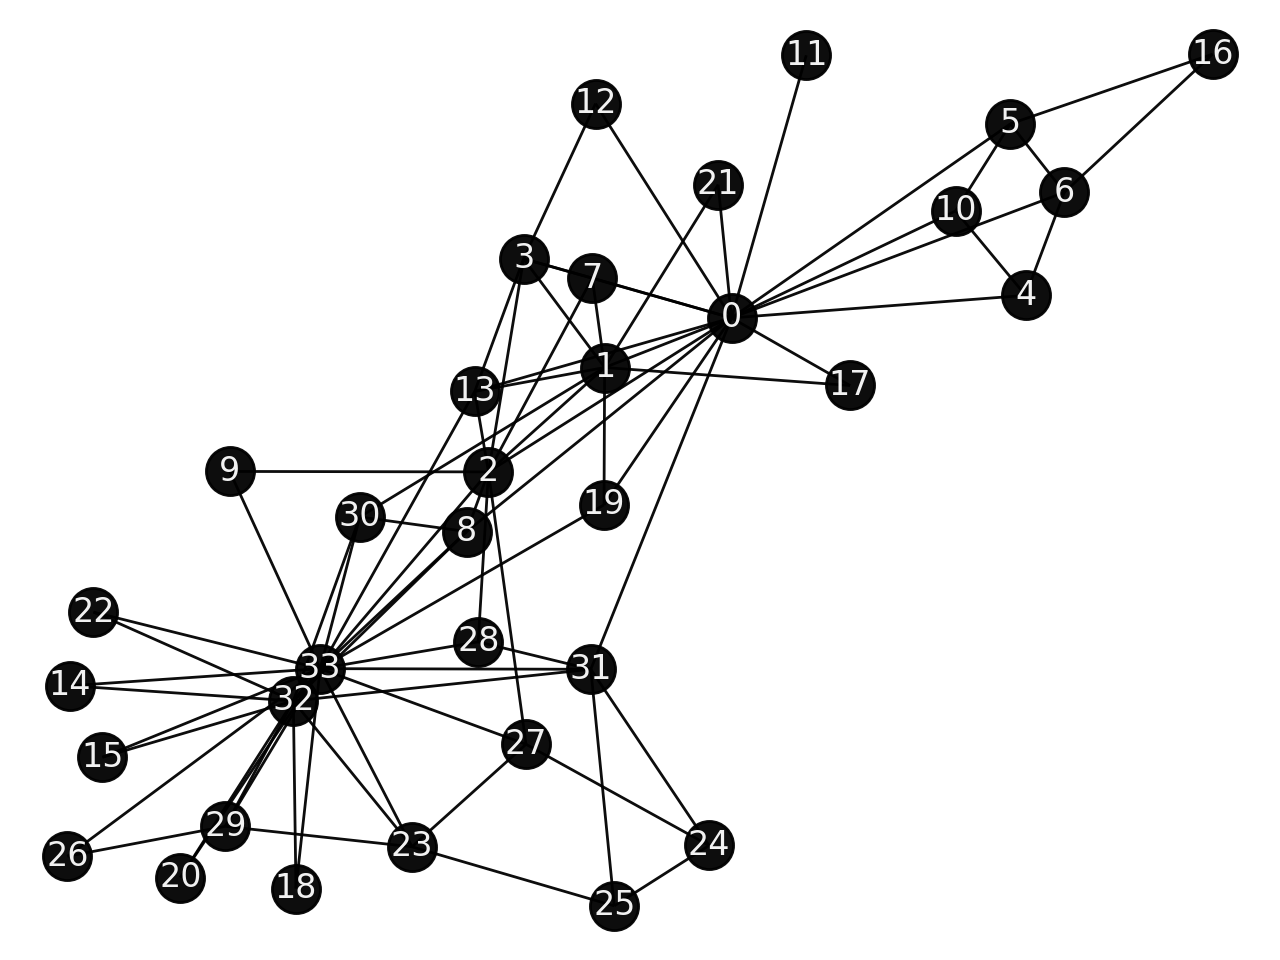
\includegraphics[width=0.6\columnwidth]{chapter3Fig/exm.png}\\
	% 
	\caption{空手道俱乐部网络}
	\label{Fig: karate}	
\end{figure}

图 \ref{Fig: karate} 是经典的空手道俱乐部网络Zachary  \cite{Zachary1977} 。该网络由34个节点构成,节点间有78条连边。
网络中,节点代表空手道俱乐部成员,节点之间的连边代表俱乐部成员之间存在某种关系。在这个网络上,实验分别最优化经典判据$ R $,耦合强度范围$ \omega $和收敛速度$ v $,穷举破解得到5个牵制控制节点;并观察分别在不同控制节点集合下,这三个指标的变化情况。实验参数设置见章节$ 3.3.3 $。

\begin{table*}[h]\centering{	
		\caption{不同的牵制节点对应三种指标的变化情况}
		\centering
		{	\begin{tabular}{cccc}
				\hline
				\hline
				 &Optimal $ R $&Optimal $ \omega $&Optimal $ v $\\ \hline
		  控制节点&[1,2,5,31,32]&[0,2,6,32,33]&[4,13,16,25,26] \\
			$ R $&\textbf{0.026} &0.025&0.015 \\
	   $ \omega $&-0.106&\textbf{-0.080}&-0.352\\
			$ v $&0.086&0.102&\textbf{0.047} \\
				\hline
				\hline	
			\end{tabular}				
			\label{table:exm}
	}}
\end{table*}

表 \ref{table:exm} 描述了不同的牵制节点对应的三种指标的变化情况。实验通过最优化传统判据$ R $,耦合强度范围$ \omega $和收敛速度$ v $,分别得到的不同的控制节点集合$ [1,2,5,31,32] $,$ [0,2,6,32,34] $和$ [4,13,16,25,26] $。
从表中可以观察到,这几个控制节点集合所对应的收敛速度$ v $均大于$ 0 $,也就是说网络中存在正的最大李亚普诺夫指数,网络无法被这些节点集合所控制。在第二列中,实验最优化传统比率判据,该控制节点集合也没有使整个网络达到最大的耦合强度范围。
通过这两点,可以很清晰地发现,传统判据无法精确衡量节点对网络的控制能力;相比较而言,耦合强度范围和收敛速度这两个指标描述得更精确一些。

\subsubsection{实验数据}
实验在斯坦福大学公开数据库上选取了4个真实网络,分别是:Italy powergrid \cite{Motter2013}, PDZBase \cite{Beuming2005}, Contiguous USA \cite{Knuth2008}和Zachary。
Italy powergrid是意大利的一个电力网络,网络中的节点代表发电机(或变压器、变电站),连边代表发电机之间存在某条供电线路。
PDZBase是一个蛋白质网络,网络的节点代表一种蛋白质,节点之间的连边代表蛋白质之间存在某种联系。
Contiguous USA是美国的州网络,网络的节点代表美国除了夏威夷和阿拉斯加外所有的州和哥伦比亚特区,节点之间连边代表两个州之间存在边界线。
Zachary 是上文提到的空手道网络。

为了便于计算,在实验过程中,所有网络被调整成无向无权重网络,并且没有自环。这6个真实网络的统计信息如表 \ref{table:chp3} 。其中,$ N $代表网络节点的个数,代表网络的连边数,$ H $代表网络节点的异质性,$ r $代表网络的同配性,$ <C> $代表网络的平均聚类系数,$ <d> $代表平均最短路径长度。

需要注意的是,这4个真实网络存在结构简单的问题。事实上,本章第二节已经证明了比率判据、耦合强度范围和收敛速度是不同的指标,同时微分分析证明了无法同时最优化这三者;这里的实验仅为验证实验。网络节点更多,结构更加复杂时,该结论也是成立的。另外,本节实验采用暴力破解计算出最优的指标值,在网络节点更多时,时间复杂度过大,无法计算。
最后,对于有向网络来说,我们的结论是不成立的;因为结论基于对称网络,对于有向网络而言,该网络是不对称的,该网络的对角化和控制部分的理论都不成立。


\begin{table*}[h]\centering{	
		\caption{四个真实网络的结构属性特征}
		\centering
		{	\begin{tabular}{ccccccc}
				\hline
				\hline
				Network&$ N $&$ E $&$ H $&$ r $&$ <C> $&$ <d> $\\ \hline
				Italy powergrid&67&93&1.175&-0.036&0.022&6.701 \\
				PDZBase&161&209&2.263&-0.460&0.001& 5.326\\
				Contiguous USA&49& 107&1.130&0.233&0.229&4.163 \\
				Zachary&34& 78&1.693&-0.476&0.074&2.408 \\
				\hline
				\hline	
			\end{tabular}				
			\label{table:chp3}
	}}
\end{table*}

\subsubsection{参数设置}
本实验采用了罗塞尔吸引子模型来模拟节点自身状态的变化情况。吸引子是指在混沌系统的相空间中存在一个点集$ s $,对于点集$ s $近邻区域的所有点,在时间趋近于正无穷时,这些点的轨迹都趋于$ s $。因此,$ s $也被称为稳定点。
罗塞尔吸引子由三个常微分方程组成,在连续的时间系统内有 \cite{Roessler1976}:
\begin{equation}
\begin{aligned}
\frac{d{x}_{i1}}{dt}&=-x_{i2}-x_{i3},
\\
\frac{d{x}_{i2}}{dt}&=x_{i1}+a_1x_{i2},
\\
\frac{d{x}_{i3}}{dt}&=a_2+x_{i3}(x_{i1}-a_3).
\end{aligned}
\label{Eq: Rossler_variation}
\end{equation}

图 \ref{Fig: rossler三维} 描述了罗塞尔吸引子在各个方向上的变化情况。其中,罗塞尔吸引子有两个固定点 \cite{Agiza2001}:
\begin{equation}
\begin{aligned}
&(\frac{a_3+\sqrt{a_3^2-4a_1a_2}}{2}, \frac{-a_3-\sqrt{a_3^2-4a_1a_2}}{2a_1}, \frac{a_3+\sqrt{a_3^2-4a_1a_2}}{2a_1})\\
&(\frac{a_3-\sqrt{a_3^2-4a_1a_2}}{2}, \frac{-a_3+\sqrt{a_3^2-4a_1a_2}}{2a_1}, \frac{a_3-\sqrt{a_3^2-4a_1a_2}}{2a_1})
\end{aligned}
\end{equation}

这两个固定点中,一个位于吸引子的中心(图 \ref{Fig: rossler三维} 的红色点),一个远离吸引点(图 \ref{Fig: rossler三维} 的绿色点)。


\begin{figure}[ht]%{.5\linewidth}
	\centering
	% Requires \usepackage{graphicx}
	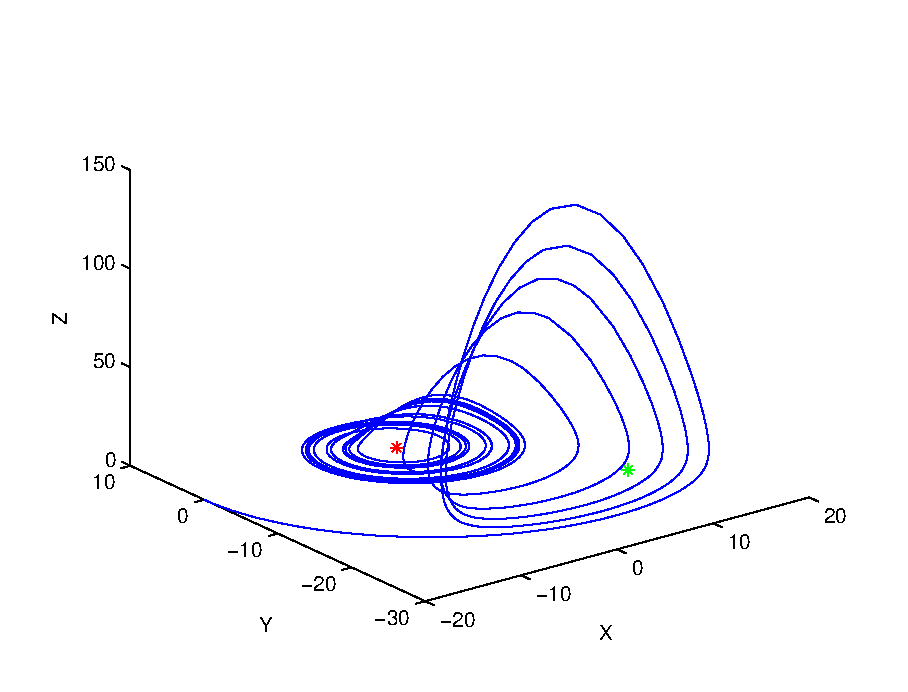
\includegraphics[width=0.7\columnwidth]{chapter3Fig/3d.eps}\\
	% 
	\caption{罗塞尔吸引子的变化情况}\label{Fig: rossler三维}	
	
\end{figure}

罗塞尔吸引子的各项参数设定为:$  a_1=0.2 $, $ a_2=0.2 $,$ a_3=5 $。
则稳定点为:$ \overline{\textbf{x}}=(0.008, -0.040, 0.040)^T $。
本实验中,节点间的耦合强度耦合强度$ c=0.3 $,节点间的耦合方式设定为$ H = [1,0,0;0,0,0;0,0,0] $,可以计算出$ \alpha_1 $与$ \alpha_2 $的值。如图 \ref{Fig: rossler} , $ (\alpha_2,\alpha_1)=(-4.991, -0.192) $。
此外,控制节点的反馈强度$ d $为网络节点的最大度减$ 1 $,即$ d = k_{max}-1 $。


\begin{figure}[ht]%{.5\linewidth}
	\centering
	% Requires \usepackage{graphicx}
	\includegraphics[width=0.5\columnwidth]{chapter3Fig/rossler.eps}\\
	% 
	\caption{最大特征值$ \Lambda_{max}$ 关于$\alpha$的函数曲线 }
	\label{Fig: rossler}	
	
\end{figure}

\subsubsection{实验结果}
图 \ref{Fig: opt_r} 描述了$ 4 $个真实网络中,传统判据$ R $、耦合强度范围$ \omega $和收敛速度$ v $最优的情况下,传统判据$ R $随控制节点比例$ \theta $的变化情况。
首先,可以明显看到,不存在两条趋势线是完全重叠的;也就是说,传统判据,耦合强度范围和收敛速度这三个指标确实是三个不同的指标,他们从不同角度去刻画了网络的牵制控制。
传统判据$ R $越大代表网络更容易受控,到达稳定状态。
在图中,随着牵制控制节点的增加,不同控制节点集合对应的传统判据也在不断地增加,节点对网络的控制能力也越强。
最后,可以看到随着控制节点比例的增加,红色线$ R_{opt} $和黑色线$ \omega_{opt} $这两个集合相差不大,但都优于蓝色线$ v_{opt} $。
尤其是在\ref{Fig: opt_r} (a) PDZBase 网络中,$ v_{opt} $和$ \omega_{opt} $差别很大。

\begin{figure}[htbp]%{.5\linewidth}
	\centering
	% Requires \usepackage{graphicx}
	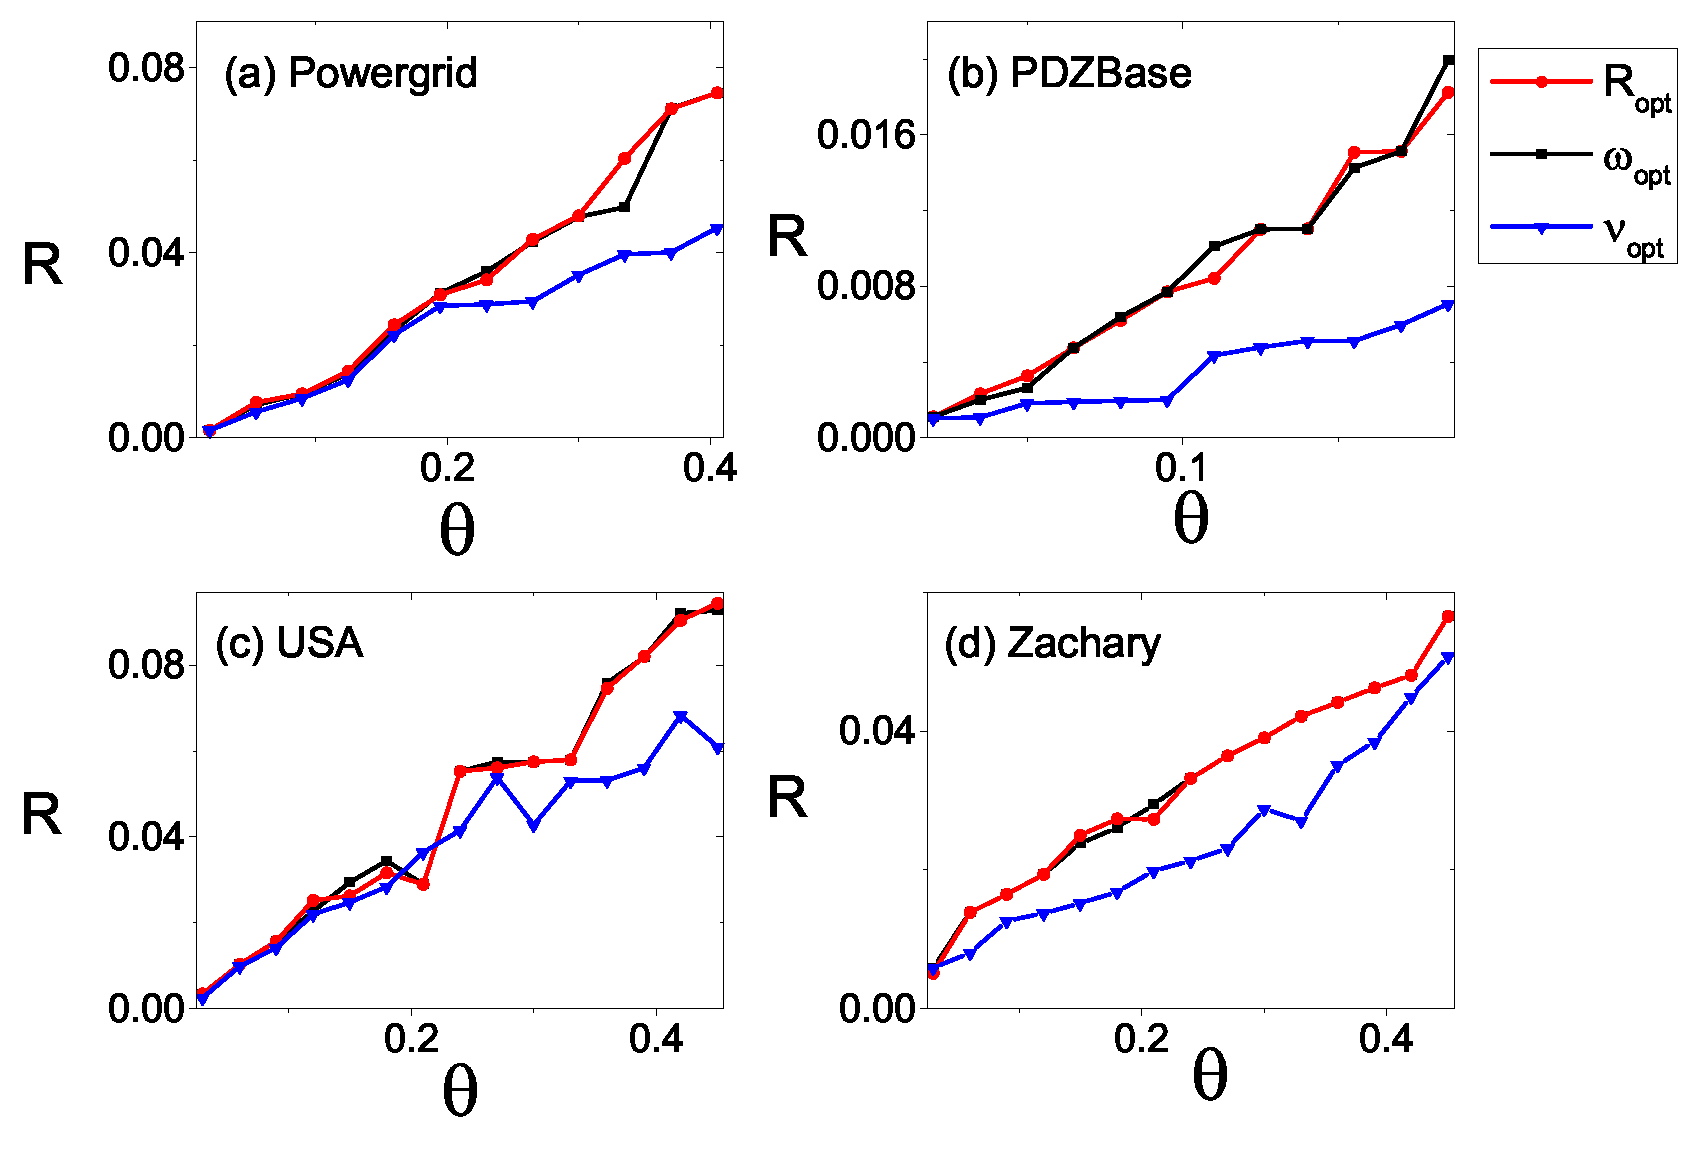
\includegraphics[width=0.9\columnwidth]{chapter3Fig/R.eps}\\
	% 
	\caption{不同网络中传统判据随控制节点比例的变化情况}
	\label{Fig: opt_r}	
	
\end{figure}

\begin{figure}[hp]%{.5\linewidth}
	\centering
	% Requires \usepackage{graphicx}
	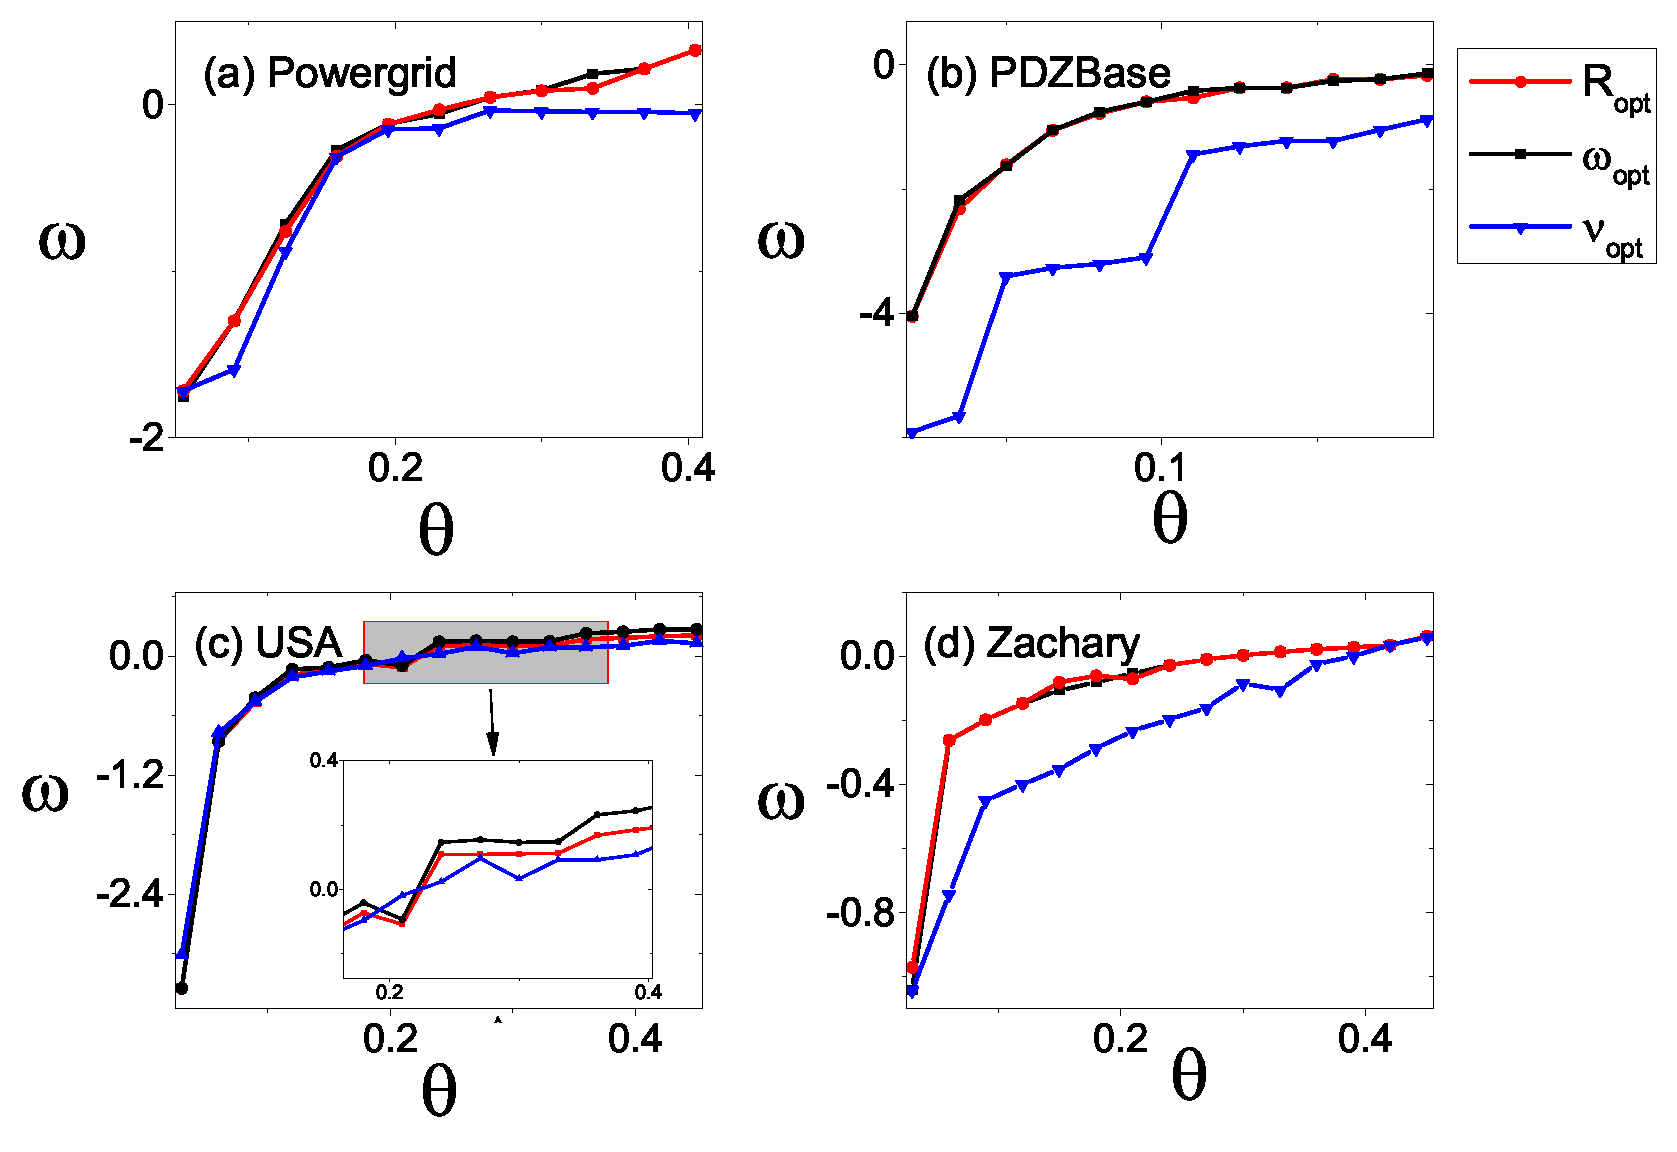
\includegraphics[width=0.9\columnwidth]{chapter3Fig/W.eps}\\
	% 
	\caption{不同网络中耦合强度范围随控制节点比例的变化情况}
	\label{Fig: opt_W}	
	
\end{figure}

\begin{figure}[hp]%{.5\linewidth}
	\centering
	% Requires \usepackage{graphicx}
	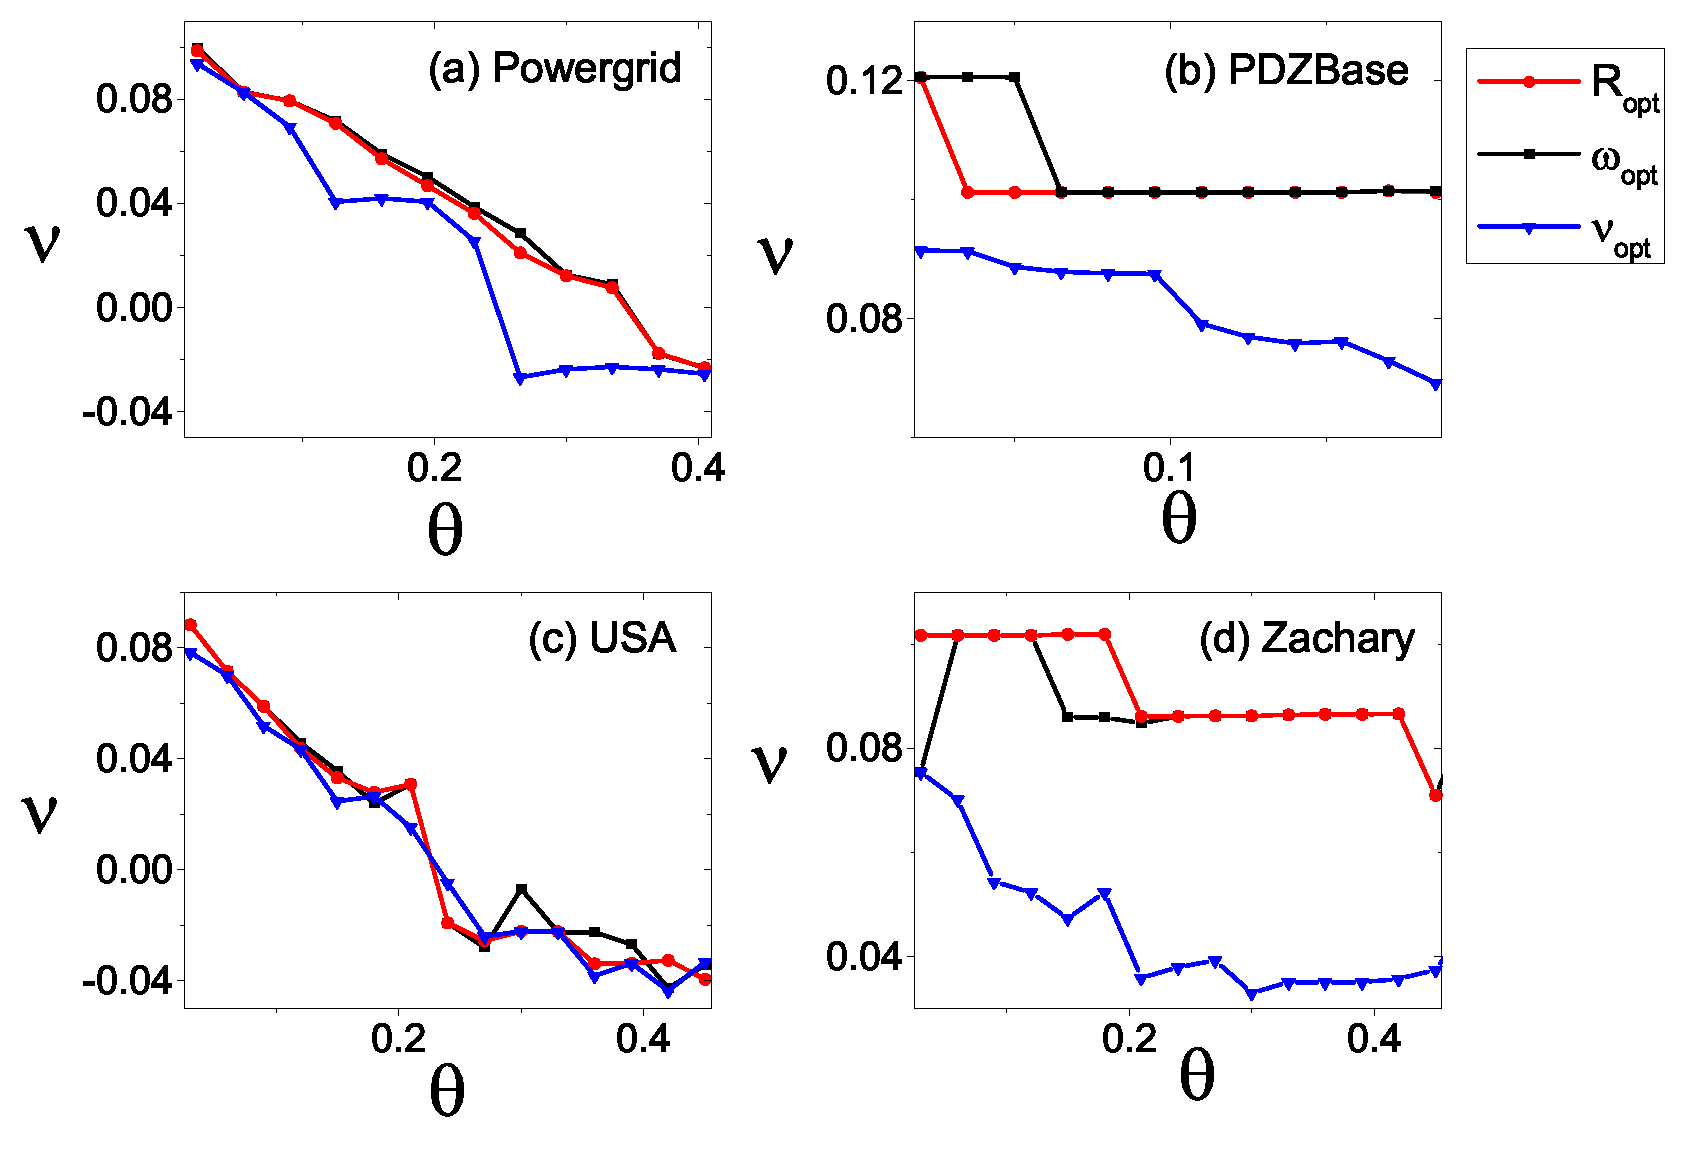
\includegraphics[width=0.9\columnwidth]{chapter3Fig/V.eps}\\
	% 
	\caption{不同网络中收敛速度随控制节点比例的变化情况}
	\label{Fig: opt_V}	
	
\end{figure}

\begin{figure}[hp]%{.5\linewidth}
	\centering
	% Requires \usepackage{graphicx}
	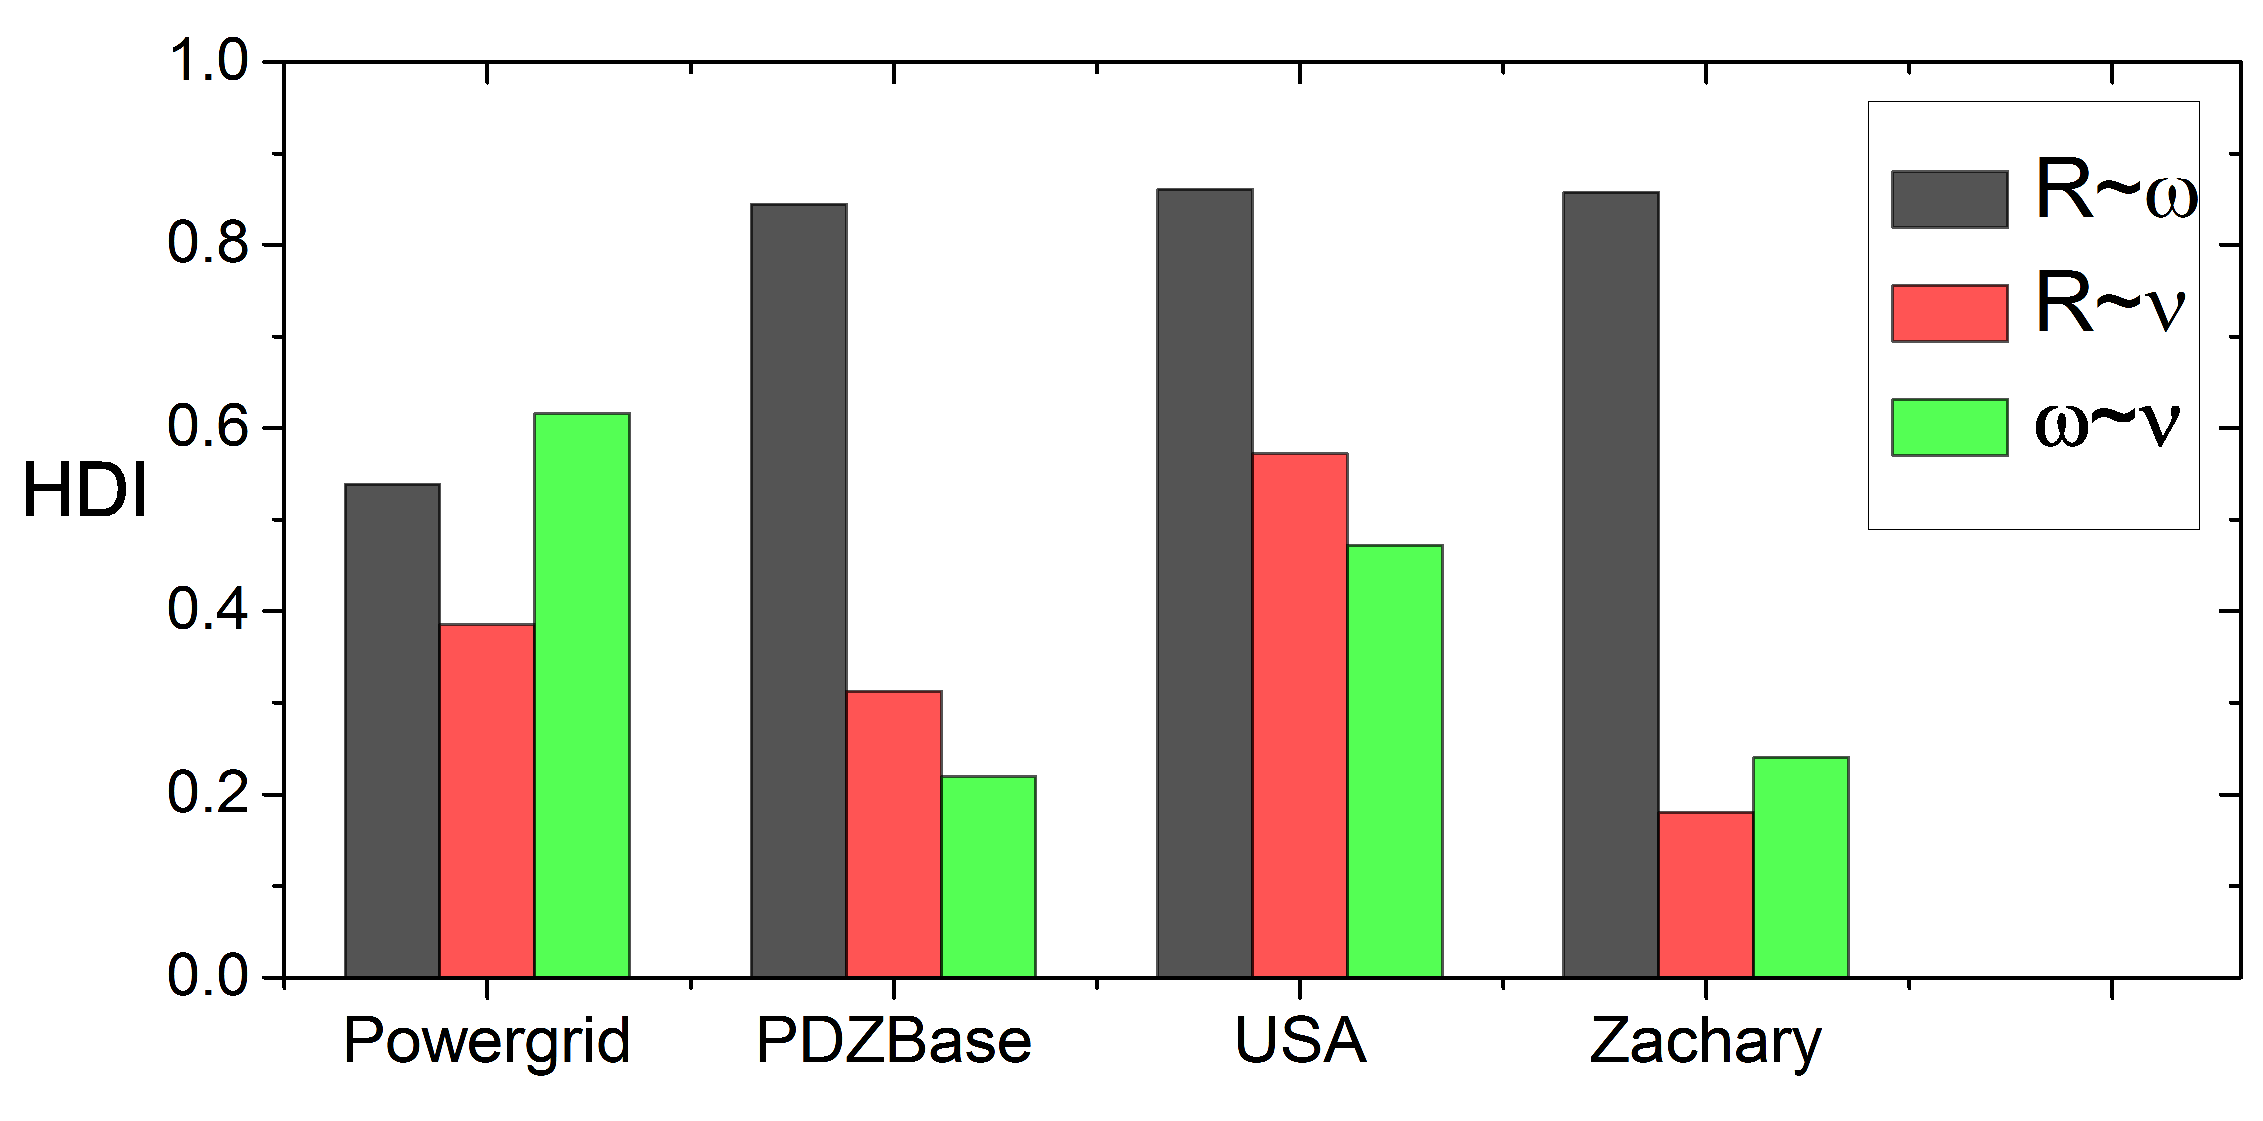
\includegraphics[width=0.8\columnwidth]{chapter3Fig/overlap.eps}\\
	% 
	\caption{不同网络中三个指标的重叠情况}
	\label{Fig: chap2overlap}		
\end{figure}

图 \ref{Fig: opt_W} 和图 \ref{Fig: opt_V} 分别描述了耦合强度范围和收敛速度随控制节点比例的变化情况。
在图 \ref{Fig: opt_W}中,耦合强度范围越大,网络更容易受控到达稳定状态。与图\ref{Fig: R}类似,红色线$ R_{opt} $和黑色线$ \omega_{opt} $相差不大,并且优于蓝色线$ v_{opt} $。
在图 \ref{Fig: opt_V}中,收敛速度$ v<0 $,且越小越好。图中可以明显看出蓝色线$ v_{opt} $优于红色线$ R_{opt} $和黑色线$ \omega_{opt} $。
可以从图 \ref{Fig: opt_r}、图 \ref{Fig: opt_W} 和图 \ref{Fig: opt_V}中归纳出,不存在一个控制节点集合(一条颜色线),同时在经典判据$ R $、耦合强度范围$ \omega $和收敛速度$ v $中达到最优。
另外需要注意的是,在图 \ref{Fig: opt_V} (a) Powergrid 网络 中,当控制节点比例$ \theta<0.2 $时,该网络的收敛速度$ v>0 $,这意味着系统中有一个正的李雅普诺夫指数,即该系统无法到达稳定状态。


总体而言,传统判据、耦合强度范围和收敛速度三个评价指标是无法同时达到最优。但是,红色线$ R_{opt} $和黑色线$ \omega_{opt} $在图 \ref{Fig: opt_r}和图 \ref{Fig: opt_W}中相差不大。这是否意味着经典判据和耦合强度范围存在比较强的相关性呢?

接下来,实验取20\%的结点作为牵制控制节点,观察不同网络中,这三个指标选择控制节点的重叠情况。如图\ref{Fig: chap2overlap},在PDZBase、USA、Zachary网络中,$ {\rm HDI}_{R~\omega}>0.8 $,这说明耦合强度范围和传统判据这两个指标在这几个网络中,相似性非常高;相比较而言,$ {\rm HDI}_{R~v} $与$ {\rm HDI}_{\omega~v} $较低一些。
需要注意的是,$ R $、$ \omega $和$ v $是三个不同的衡量指标,他们分别从不同角度去说明了网络的牵制控制问题。



\subsection{本章小结}
本章从经典网络控制问题出发,提出了衡量节点对网络牵制控制的传统比率判据。但实验发现,传统判据无法精确描述牵制控制,因此提出了耦合强度范围和收敛速度两个指标。前者决定了网络受控稳定时耦合强度的大小,后者则从网络的拓扑结构方面,给出了系统受控稳定时的收敛速度。同时,本章在理论上分析了传统判据、耦合强度范围和收敛速度无法同时到达最优,并在实验中给出了验证。


\clearpage

\section{重要节点检测算法在牵制控制上的研究}

第四章主要研究重要节点检测算法及算法在牵制控制上的应用。
传统重要节点检测算法在网络牵制控制中,往往效果不稳定,在不同的网络中差异巨大。
为了解决这个问题,本章对耦合强度范围这一指标进行扰动分析,衡量了单节点和多节点重要性,提出了一个网络重要节点检测算法。
该算法复杂度低,能够有效地计算出网络中的重要节点。
在六个真实网络中的实验显示,该算法容易找到被其他算法所忽视的重要节点,能够极大地增强节点对网络的控制能力。

\subsection{耦合强度范围的扰动研究}

本节分析耦合强度范围的扰动,首先从单一节点出发,选取影响能力最大的节点作为网络重要节点;同理,在多节点重要性衡量时,在误差允许的范围内,可以根据耦合强度范围的扰动情况,选取最佳的节点集合。
随后依据重要节点的检测过程,本章提出了一个贪婪算法,该算法复杂度低,能够快速计算出网络的重要节点,并给出了算法伪代码。

\subsubsection{单节点的重要性检测}

当控制网络中单个节点$ i $时,通过耦合强度范围的微分(见式子 \ref{Eq:orginperturb2} ),可以近似地计算出该节点所引起耦合强度范围的扰动:
\begin{equation}
\begin{aligned}
\Delta \omega  &= d\frac{\partial \omega}{\partial d_i}
\\
&\approx \frac{d}{\lambda_1^2}[\alpha_2R^2(X_N^i)^2-\alpha_1(X_1^i)^2]. 
\end{aligned}
\label{Eq: Delta_omega}
\end{equation}

大部分情况下,反馈强度$ d $被设置为一个固定值。因此,对于某个节点$ i $来说,定义$ PW $值:
\begin{equation}
PW(i) \approx \frac{1}{\lambda_1^2}[\alpha_2R^2(X_N^i)^2-\alpha_1(X_1^i)^2].
\label{Eq: PWi}
\end{equation}
其中,$ i $代表新增的某一控制节点,常数$ \alpha_1 $和$ \alpha_2 $与网络模型以及节点间的耦合方式有关,$ R $指的是未加控制节点$ i $前网络的传统比率判据,$ (X_1^i) $和$ (X_N^i) $代表特征向量$ X_1 $和$ X_N $的第$ i $个元素值,特征向量$ X_1 $和$ X_N $分别与控制矩阵$ C $(见式子\ref{Eq: C})的最大最小特征值$ \lambda_1 $和$ \lambda_N $对应。

节点的$ PW $值反映了该节点作为控制节点时对耦合强度范围的影响。$ PW $值越大,代表影响越大,耦合强度范围的变化更为剧烈,也就是说这个节点对耦合强度范围而言也更为重要。需要注意到的是,在大多数情况下,$ \alpha_2<<\alpha_1\approx0 $,节点的$ PW $值主要由式子$ \ref{Eq: PWi} $第一项来决定;但是在实验中发现,式子第二项对节点的$ PW $值仍有较大影响。

\subsubsection{多节点的重要性检测}

这节在单个节点对耦合强度范围的扰动的基础上,探究多个节点对耦合强度范围的影响。
当一小部分节点$ P=\{x_1,x_2,...,x_u\} (u<<N) $作为网络的牵制控制节点时,同样忽略二阶导数项,
%,在忽略了二阶导数的情况下,当一小部分节点$ P=\{x_1,x_2,...,x_u\} (u<<N) $作为网络的牵引控制节点时,
式子\ref{Eq: Lambda_eigenvector}可以改写成:
\begin{equation}
\frac{\partial\lambda_k}{\partial{d_P}} = -\sum_{i=1}^{u}(X_k^{i})^2.
\label{Eq: multiplenode}
\end{equation}
将式子\ref{Eq: multiplenode}带入耦合强度范围$ \omega $的微分中,可以得到:
\begin{equation}
\begin{aligned}
PW(P) \approx  -\frac{1}{\lambda_1^2}[\alpha_1  \sum_{i=1}^{u}{(X_1^{i})^2}-\alpha_2 R^2 \sum_{i=1}^{u}{(X_N^{i})^2}].
\end{aligned}
\label{Eq: PWP}
\end{equation}

式子 \ref{Eq: PWP} 描述了多个节点作为网络的牵制控制节点时,耦合强度范围的变化情况。同样,$ PW $值越大,代表节点集合产生的耦合强度范围扰动越大,在反馈强度$ d $不变的情况下,该节点集合所对应的耦合强度范围也就越大。
而网络的稳定状态和耦合强度范围呈正相关关系,因此该节点集合更合适当作控制节点。
在工程上,可以通过选择拥有最大$ PW $值的节点集合作为控制节点,获得尽可能大的牵制强度范围。


\subsection{算法伪代码}

本节关注于如何通过节点的$ PW $值找到最佳的控制节点集合,从而确定网络的重要节点。
总体而言,耦合强度范围的变化源于每个控制节点影响的叠加,而每个控制节点的影响可以用节点的$ PW $值来衡量。因此,可以采用贪婪算法的思想,迭代地找出局部最优节点。在每次迭代过程中,可以选择具有最大$ PW $值的节点,作为当前情况下的最佳控制节点。并在多次的迭代过程中,找到最佳控制节点集合。

算法的流程如下:

(1)给定一个网络$ G(V,E) $,节点自身的动力学方程$ f(x) $,耦合矩阵$ H $;

(2)保证李雅普诺夫指数$ L_{max} $小于0的情况下,计算$ \alpha_1 $和$ \alpha_2 $;

(3)控制节点集合$ P $的初始化,将$ P $设置为空集;

(4)得到牵制控制矩阵$ C $,并计算$ C $的最大最小特征值$ \lambda_1 $与$ \lambda_N $和与之对应的特征向量$ X_1 $与$ X_N $;

(5)计算每个节点的$ PW $值并排序,选取拥有最大$ PW $值且不属于$ P $的节点,将其作为新增的控制节点;

(6)重复步骤4-5,直到满足控制节点的个数。

算法的伪代码如下:
\floatname{algorithm}{算法}
\label{algorithm}
\renewcommand{\algorithmicrequire}{\textbf{输入:}} 
\renewcommand{\algorithmicensure}{\textbf{输出:}}
\begin{algorithm}[htp]
	\caption{基于耦合强度范围扰动的关键节点算法}
	\label{PWcode}
	\begin{algorithmic}[1]
		\REQUIRE
		原始网络$ G(V,E) $,包含$ N=|V| $个节点和$ |E| $条边;
		节点自身的动力学方程$ f(x) $;
		节点之间的耦合矩阵$ H $;
		控制节点个数$ u $。
		\ENSURE
		控制节点集合$ P $。
		\STATE 确保$ \Lambda_{max}[Df+\alpha H]<0 $的情况下,计算$ (\alpha_2, \alpha_1) $的值
		\STATE 初始化节点集合$P=\emptyset $
		\REPEAT
		\STATE 牵制控制矩阵$ C=-L-D $
		\STATE 计算牵制控制矩阵$ C $的最大最小特征值$ \lambda_1 $和$ \lambda_N $,及与之相对应的特征向量 $ X_1 $和$ X_N $
		\STATE 计算经典比率判据$ R = {\lambda_1}/{\lambda_N} $%compute classical metric ratio				
		\FOR{网络的每个节点$ i=1 $ 至 $ n $}
		\STATE  计算每个节点的$ PW $值$ PW(i) =  \frac{1}{\lambda_1^2}[\alpha_2R^2(X_1^i)^2-\alpha_1(X_N^i)^2] $
		\ENDFOR
		\STATE 选择拥有最大$ PW $值且不属于$ P $的节点$ m $
		\STATE 将点$ m $加入控制节点集合$ P $
		\UNTIL{节点集合$ P $的元素个数等于$ u $}
		\STATE 返回控制节点集合$P$
	\end{algorithmic}
\end{algorithm}

算法伪代码中,$ L $和$ D $等参数的定义已在第三章第一节稳定性分析部分给出;循环计算出新的节点后,牵制控制矩阵$ C $依然会执行$ i=1 $ 至 $ n $的循环,在实际代码过程中可以简便地用一个临时值减少循环次数。另外,不同重要节点检测算法的时间复杂度见表 \ref{table:oo} 。从表中可以看到,和其他算法相比,基于耦合强度范围扰动算法(PW方法)时间复杂度较低,较易计算出网络重要节点。

\begin{table*}[h]\centering{	
		\caption{不同算法时间复杂度比较}
		\centering
		{	\begin{tabular}{cc}
				\hline
				\hline
				算法&时间复杂度\\ \hline
				度中心性(Degree centrality)&$ O(n) $ \\
				介数中心性(Betweenness centrality)&$ O(n^3) $ \\
				接近中心性(Closeness centrality)&$ O(n^2) $ \\
				特征向量中心性(Eigenvector centrality)&$ O(n^2) $\\
				K-shell分解算法(Closeness centrality)&$ O(n^2) $\\
				PageRank&$ O(n^2) $ \\
				ESI方法&$ O(n) $ \\
				基于耦合强度范围扰动算法(PW方法)&$ O(nk) $ \\
				\hline
				\hline	
			\end{tabular}				
			\label{table:oo}
	}}
\end{table*}


\subsection{性能评估}
实验先在仿真网络上给出一个示例,说明基于耦合强度扰动方法的有效性。接下来在6个真实网络上进行了模拟实验,将提出的基于耦合强度范围扰动的算法与其他5个经典算法进行了对比分析,同时追踪观察节点的状态变化情况,从而验证了基于耦合强度范围算法的准确性。另外,实验还给不同算法得到的控制节点集合做了重叠性分析,并比较了不同算法下耦合强度范围和经典判据之间的相关关系。

\subsubsection{仿真网络上的示例}

\begin{figure}[ht]%{.5\linewidth}
	\centering
	% Requires \usepackage{graphicx}
	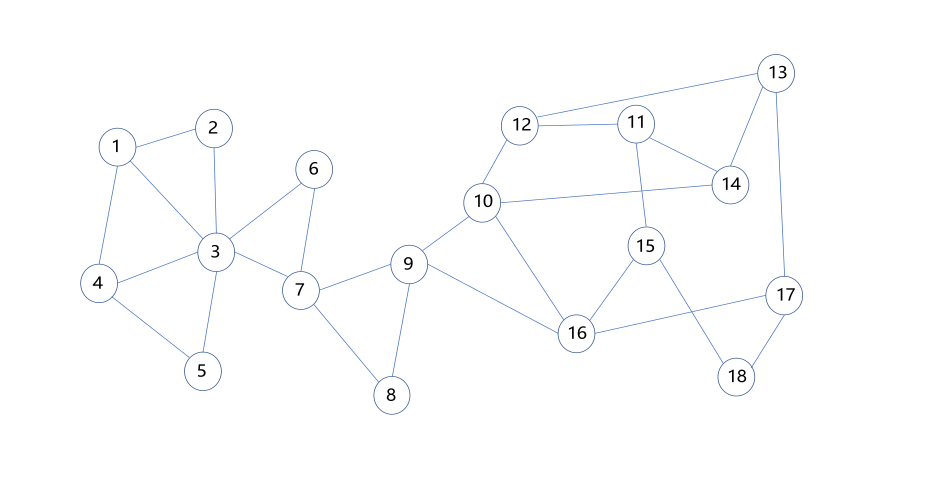
\includegraphics[width=0.8\columnwidth]{chapter4Fig/exm.png}\\
	% 
	\caption{一个仿真网络}
	\label{Fig: man-made}	
	
\end{figure}

图 \ref{Fig: man-made} 是一个仿真网络,该网络由$ 18 $个节点和$ 27 $条边构成。在这个网络上,通过不同算法计算出网络的重要节点和耦合强度范围。具体实验参数见章节 $ 4.3.3 $。

\begin{table*}[h]\centering{	
		\caption{不同算法选择的控制节点和耦合强度范围的比较}
		\centering
		\begin{tabular}{|c|c|c|}
			\hline
			算法&控制节点集合&耦合强度范围\\\hline
			\textbf{PW} 方法&(1,5,8,11,13,17)&\textbf{0.248}\\\hline
			ESI 方法&(1,2,3,4,5,7)&-2.293\\\hline
			度中心性&(1,3,7,9,10,16)&-0.098\\\hline
			介数中心性&(3,7,9,10,15,16)&0.034\\\hline
			接近中心性&(3,7,8,9,10,16)&-0.096\\\hline
			PageRank&(3,7,9,10,12,16)&0.040\\\hline	
		\end{tabular}				
		\label{table:different_al}
	}
\end{table*}

表 \ref{table:different_al} 描述了不同算法选择的控制节点集合和对应的耦合强度范围。 从表中可以明显看出,PW算法选择了控制节点集合(1,5,8,11,13,17),这组节点集合对应的耦合强度范围最大;也就是说PW算法效果更好,能够获得更大的耦合强度范围,促进节点对网络的控制作用。
其次是PageRank和介数中心性算法。这两个算法对应的耦合强度范围都大于0;也就是说,耦合强度在满足某些条件下,这些算法所对应的牵制节点能够控制整个网络。
与此相反,ESI算法、度中心性算法和最近邻算法选择的节点对应的耦合强度范围小于0;这也意味着不存在一个耦合强度,使网络达到稳定的状态。

\subsubsection{数据描述}
实验在斯坦福大学公开数据库上选取了6个真实网络,分别是:Italy powergrid, Moreno \cite{Coulomb2005}, Roundworm \cite{Duch2005}, Maayan \cite{FAA}, Facebook \cite{Viswanath2009} 和 Petster \cite{2017}。
Moreno和Roundworm分别代表的是酵母细胞中的蛋白质网络和蛔虫的蛋白质网络。蛋白质网络中,网络的节点代表蛋白质,节点之间的连边代表蛋白质之间存在某种代谢作用。Maayan则是由美国国家飞行数据中心(NFDC)采集的航空网络,该网络的节点代表机场(或服务站),连边代表NFDC所推荐的飞行路径。Facebook是社交网络,网络的节点代表Facebook用户,连边代表账户间存在相互关注关系。Petster也是社交网络,网络的节点代表在该网站上注册的宠物信息,连边代表宠物间存在朋友(或亲属)关系。

为了便于计算,在实验过程中,所有网络被调整成无向无权重网络,并且没有自环。该6个真实网络的统计信息如表\ref{table:chp4},其中,$ N $代表网络节点个数,代表网络连边数,$ H $代表网络节点的异质性,$ r $代表网络的同配性,$ <C> $网络平均聚类系数,$ <d> $代表平均最短路径长度。

\begin{table*}[h]\centering{	
		\caption{六个真实网络的结构属性特征}
			\centering
			{	\begin{tabular}{ccccccc}
					\hline
					\hline
					Network&$ N $&$ E $&$ H $&$ r $&$ <C> $&$ <d> $\\ \hline
					Italy powergrid&67&93&1.175&-0.036&0.022&6.701 \\
					Moreno&1458&1948&2.667&-0.210&0.010& 6.812\\
					Maayan&1226& 2408&1.873&-0.015&0.012&5.929 \\
					
					Facebook&744& 30023&1.633&0.503&0.559&2.558 \\
					Roundworm&453&2025&4.485&-0.226&0.098&2.664 \\
					Petster&706&10064&1.549&0.035&0.400&2.737 \\
					\hline
					\hline	
				\end{tabular}				
				\label{table:chp4}
	}}
\end{table*}

\subsubsection{对比方法与参数设置}
实验中共用选取了5种重要节点检测算法作为对比方法,分别是:度中心性(Degree centrality)、介数中心性(Betweenness centrality)、接近中心性(Closeness centrality)、PageRank算法和ESI方法。

另外,实验继续采用罗塞尔吸引子模型来模拟节点自身状态的变化情况。罗塞尔吸引子各项参数设定为:$  a_1=0.2 $, $ a_2=0.2 $,$ a_3=5 $,节点间耦合方式$ H = [1,0,0;0,0,0;0,0,0] $,则稳定点为$ \overline{\textbf{x}}=(0.008, -0.040, 0.040)^T $,$ (\alpha_2,\alpha_1)=(-4.991, -0.192) $。
在不另外声明的情况下,耦合强度$ c=0.3 $,反馈强度$ d $取网络中节点的最大度减一。动力学中方程中,节点振动频率为$ 10000 $赫兹。

\subsubsection{实验结果及分析}
首先,耦合强度取$ c=0.48 $,在Italy powergrid数据集上,不同重要节点检测算法各选取了25个节点作为牵制控制节点。在节点演化过程中,追踪了该网络上三个节点的状态变化过程,这三个节点分别是最大度节点、最小度节点和平均度节点。图 \ref{Fig: perturbation} 描述了在罗塞尔吸引子$ x_{i1} $方向上状态变化的情况。
从图中可以看到,只有在PW算法选择的控制节点下(图 \ref{Fig: perturbation} (a)),三个节点的状态在$ time>0.04 $后在$ X_{i1} $方向上是收敛的,也就是说,该网络中的节点是稳定的。对比而言,其他算法所控制的网络节点一直在震荡,无法收敛并达到稳定状态。另外,PW算法对应的耦合强度范围大于$ 0 $且最大,其他算法的耦合强度范围小于$ 0 $;所有算法对应的传统比率判据都大于$ 0 $,但PW算法的传统比率判据最大。这一方面说明PW算法效果最好,能够有效地找到牵制控制节点;另一方面也说明了耦合强度范围相较于传统判据,在描述网络牵制控制上更为有效一些。

\begin{figure}[ht]%{.5\linewidth}
	\centering
	% Requires \usepackage{graphicx}
	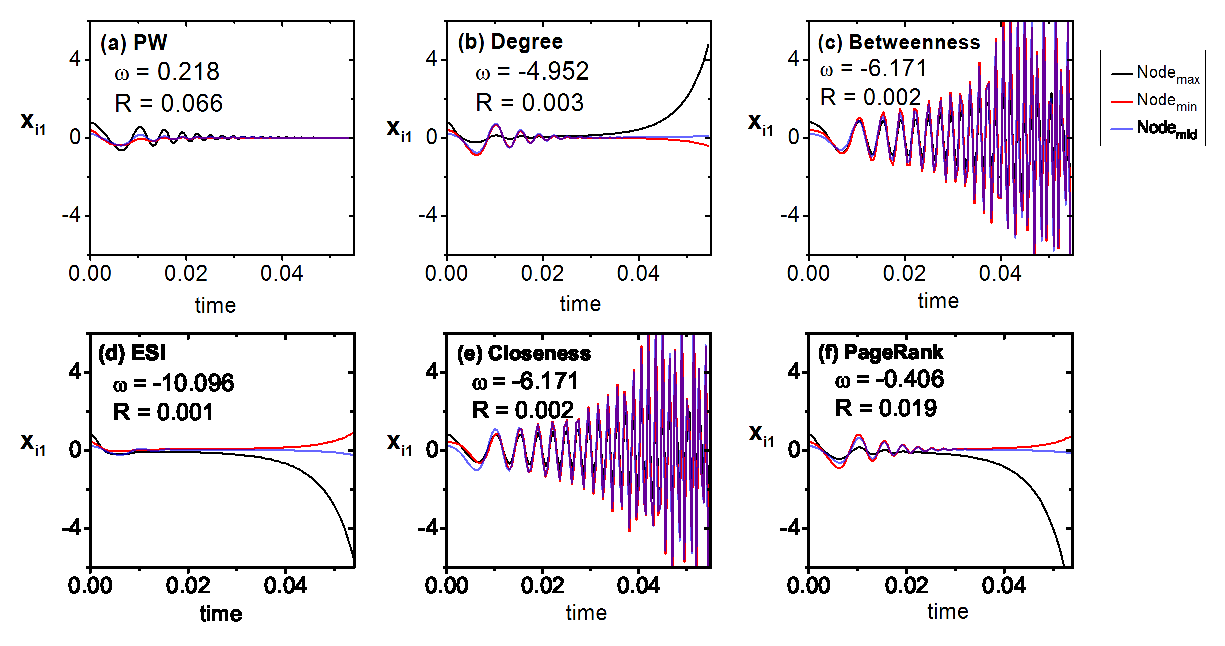
\includegraphics[width=1\columnwidth]{chapter4Fig/perturbation.eps}\\
	% 
	\caption{Italy powergrid数据集上不同方法选择节点的扰动情况}
	\label{Fig: perturbation}	
	
\end{figure}


随后,来具体观察不同网络中不同算法的实际表现情况。
图 \ref{Fig: omega} 描述了控制节点增加时耦合强度范围的变化情况。
部分情况下,随着控制节点的增加,耦合强度范围在不断扩大,网络更容易受到控制(如(a) Italy powergrid网络);同时,也存在耦合强度范围基本维持不变的情况(如(e) Roundworm网络中度中心性算法和ESI方法),因为这些算法没有选择有效的控制节点。
除此之外,在控制节点数量确定时,相较于其他启发式算法,PW算法在大部分情况下都能够获得最大的耦合强度范围。相对比而言,其他启发式算法的表现极不稳定,如在(b) Maayan网络中,牵制控制节点比例大于$ 0.2 $时,介数中心性算法和PageRank算法能获得相近的耦合强度范围,但在(d) Facebook网络中,这两种算法差异很大。由此,可以得到结论:PW算法能够稳定地得到较优的牵制控制节点集合。

\begin{figure}[htb]%{.5\linewidth}
	\centering
	% Requires \usepackage{graphicx}
	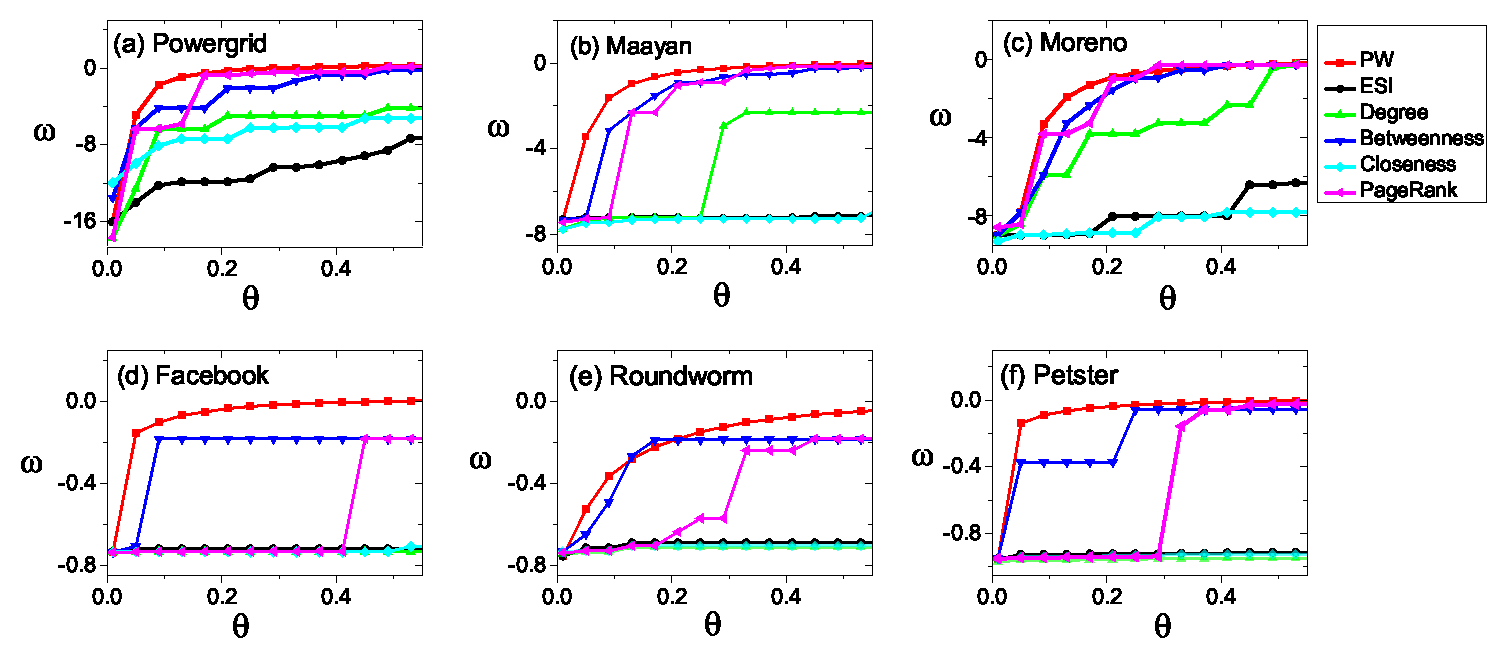
\includegraphics[width=1\columnwidth]{chapter4Fig/omega.eps}\\
	% 
	\caption{六个数据集上耦合强度范围跟随控制节点比例的变化情况}
	\label{Fig: omega}	
	
\end{figure}

同时,实验还以传统比率判据作为纵坐标,观察不同算法选择的重要节点对网络牵制控制的影响情况。图 \ref{Fig: R} 描述了不同网络在牵制控制节点比例增加时传统比率判据的变化情况。很明显,在牵制控制节点比例固定时,PW算法所对应的传统比率判据最高,也就是说,PW算法选择的牵制节点更容易控制网络。相比较而言,其他启发式算法也很不稳定,例如:在图 \ref{Fig: R} (a)中,PageRank和介数中心性算法在控制节点比例增加时,传统比率判据$ R $也在增加,也就是说,这两种算法选择的控制节点对网络的控制能力是不断增强的;但在图 \ref{Fig: R} (d)中,PageRank和介数中心性算法的比率判据的值却变化不大。由此,可以得到结论,PW算法在传统比率判据作为评判标准时,也是能够得到较优的控制节点集合的。

\begin{figure}[ht]%{.5\linewidth}
	\centering
	% Requires \usepackage{graphicx}
	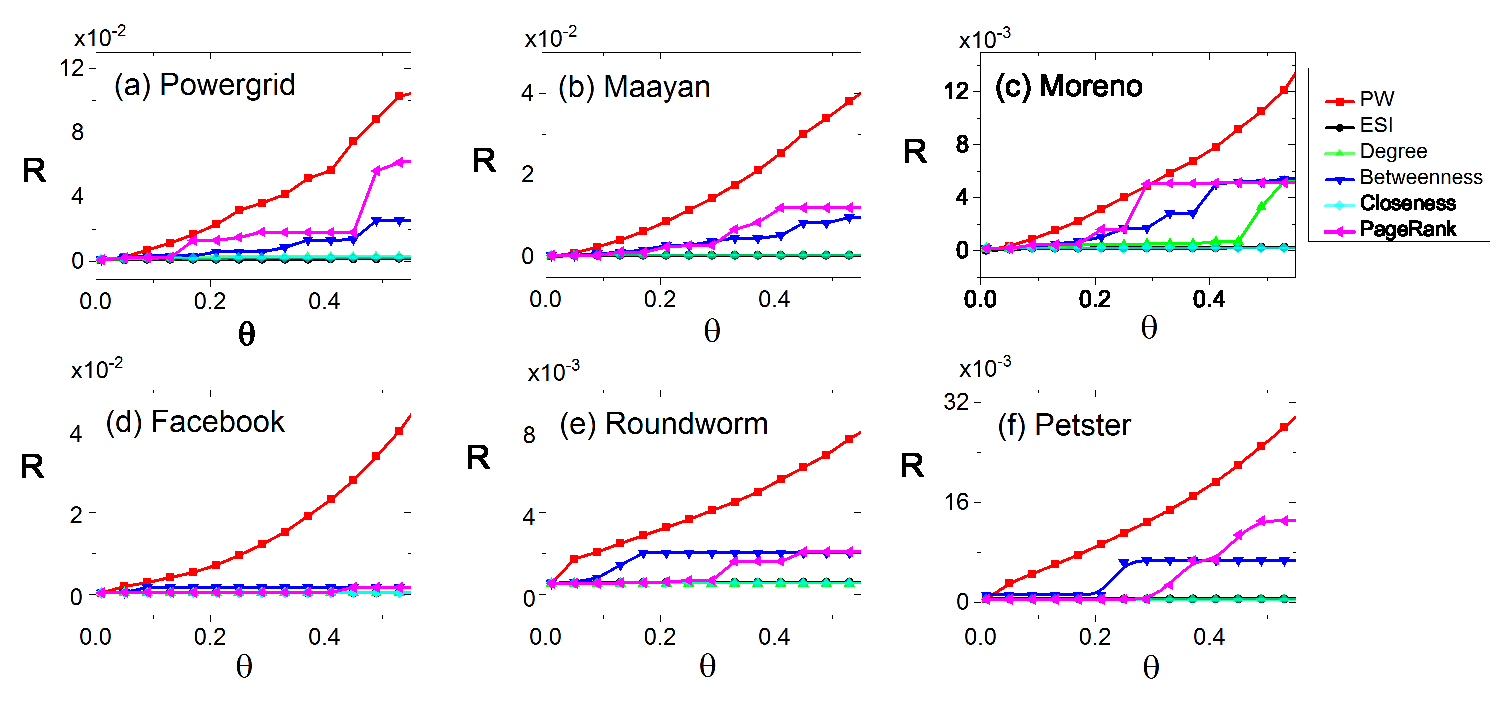
\includegraphics[width=0.9\columnwidth]{chapter4Fig/R.eps}\\
	% 
	\caption{六个数据集上传统比率判据跟随控制节点比例的变化情况}
	\label{Fig: R}	
\end{figure}

为了进一步探究$ PW $算法会选择什么样的节点作为控制节点,实验选取了30\% $ (\theta=0.3) $的节点作为控制节点,图 \ref{Fig: hdi} 描述了不同网络中PW算法和其他重要节点检测算法选择控制节点的重叠情况。从图中可以看出,六个网络中控制节点的重叠比例$ {\rm HDI}<0.3 $;也就是说,PW算法可能更倾向于选择那些容易被传统算法所忽略的节点作为控制节点。一般而言,传统方法只针对于网络或节点的某一方面特征,而且没有考虑到耦合强度范围这个指标;更重要的是,在网络控制模型中,找到最优的控制节点集合也是一个NP-hard问题。
PW算法能够快速稳定且较优地找到网络控制的重要节点,增加网络的耦合强度范围,能够很好的应用在工程中。

\begin{figure}[ht]%{.5\linewidth}
	\centering
	% Requires \usepackage{graphicx}
	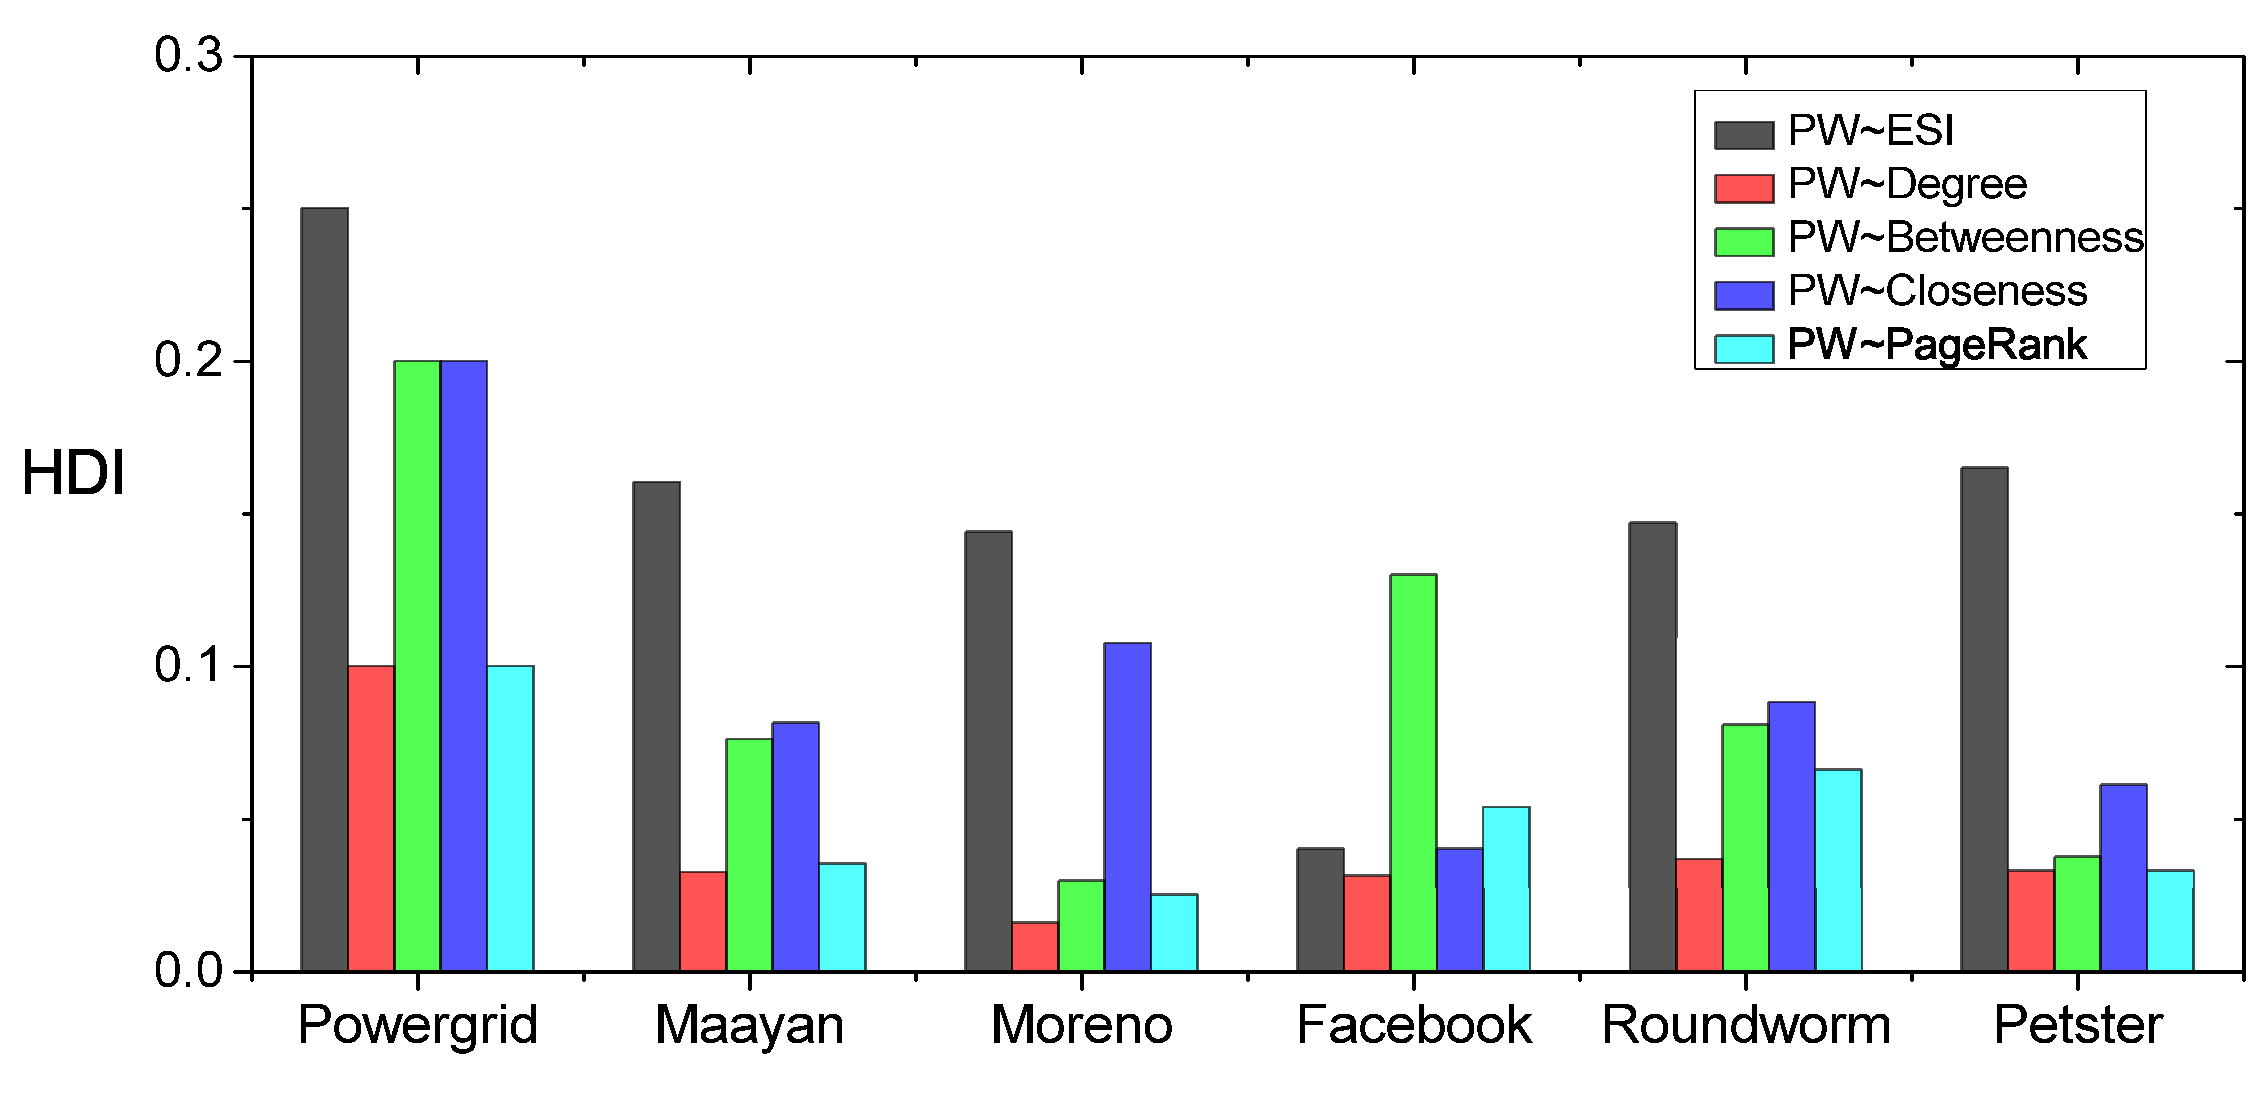
\includegraphics[width=0.9\columnwidth]{chapter4Fig/hdi.eps}\\
	% 
	\caption{六个数据集上不同方法选择节点集合的重叠情况}
	\label{Fig: hdi}	
	
\end{figure}
\begin{figure}[ht]%{.5\linewidth}
	\centering
	% Requires \usepackage{graphicx}
	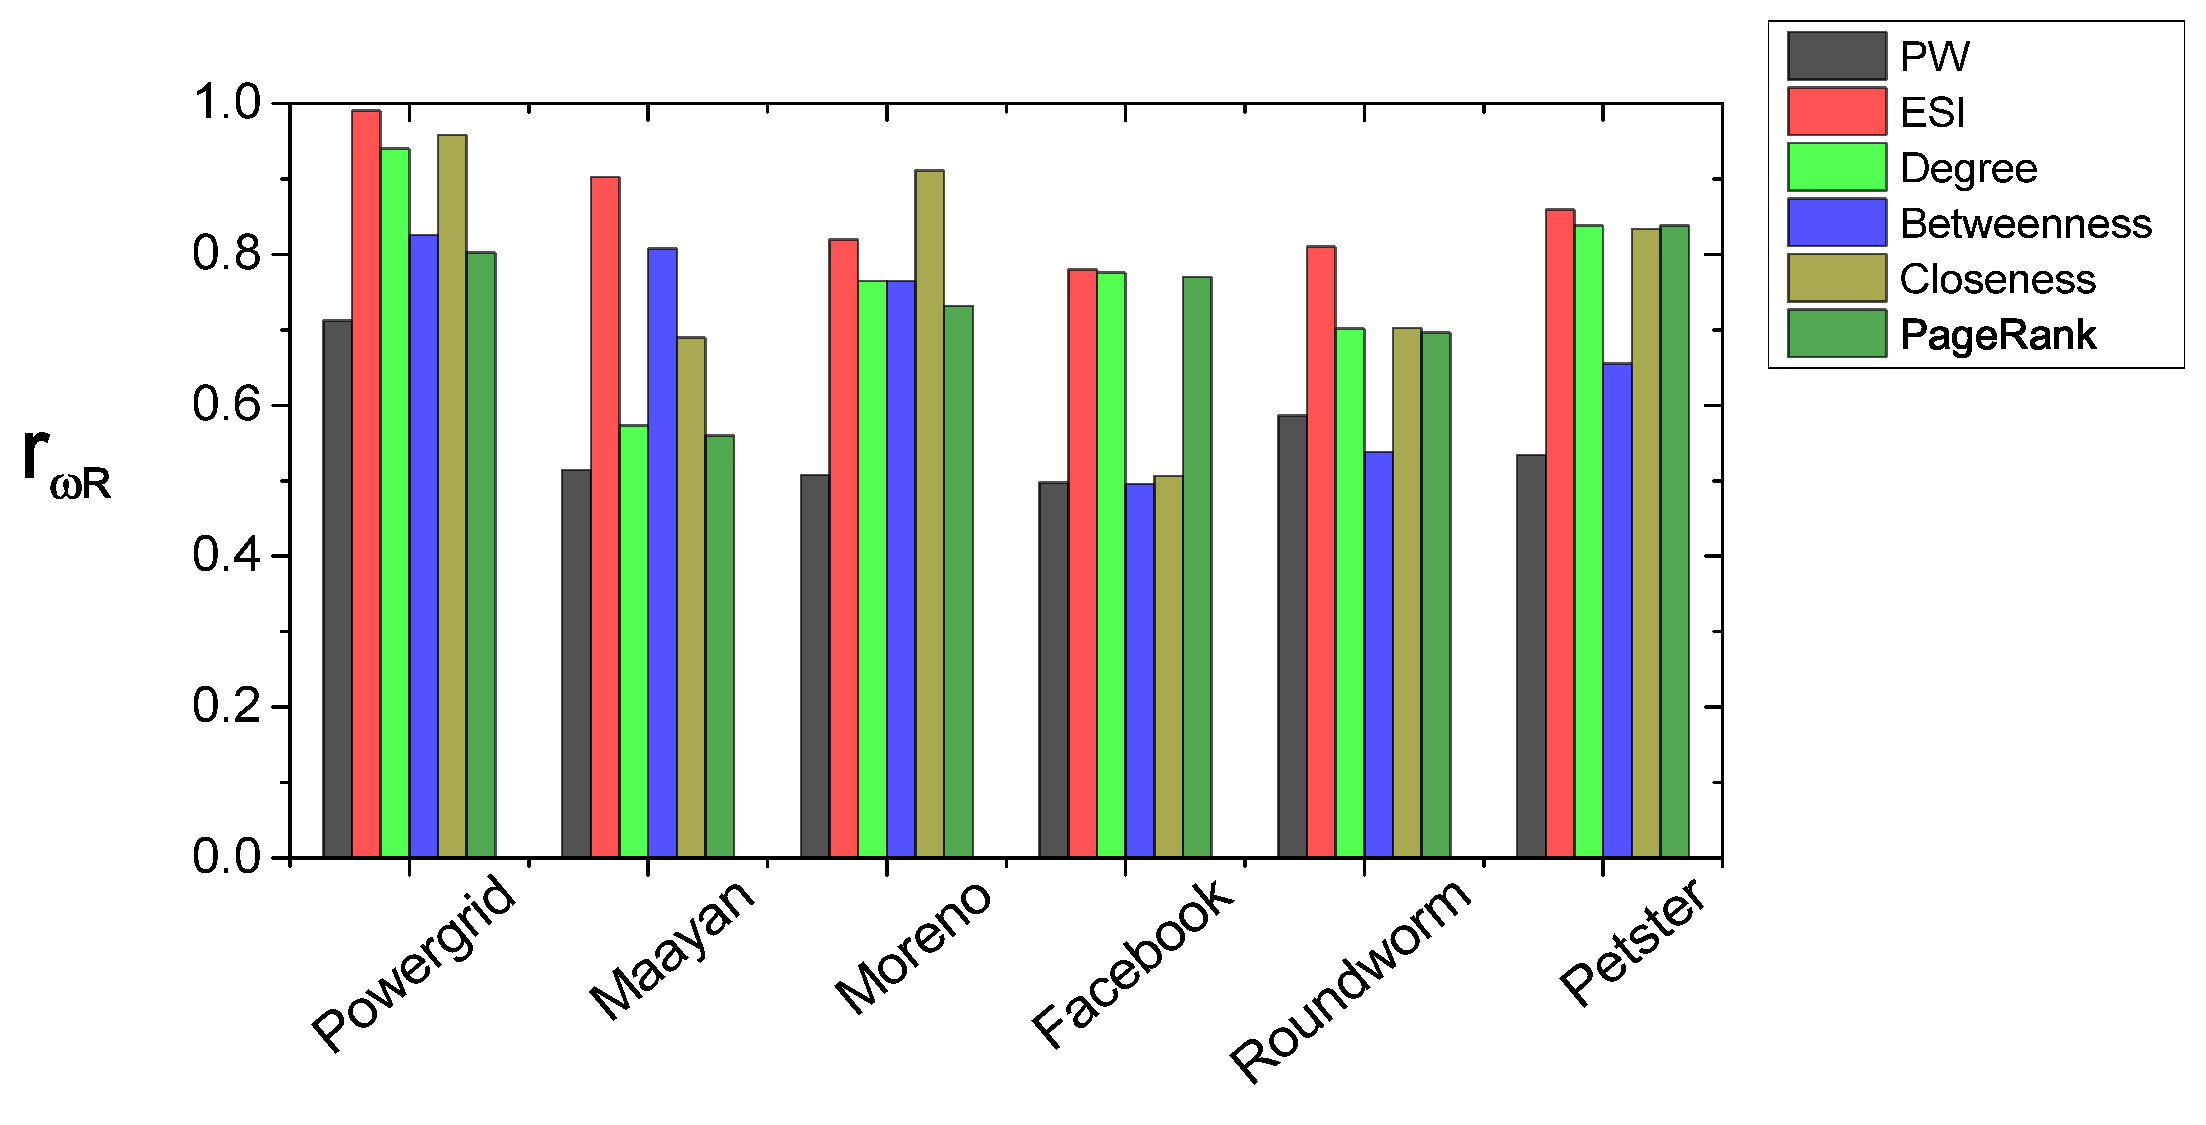
\includegraphics[width=0.9\columnwidth]{chapter4Fig/pearson.eps}\\
	% 
	\caption{六个数据集上耦合强度范围和传统比率判据的皮尔森系数}
	\label{Fig: pearson}	
	
\end{figure}

最后,实验还分析了不同网络中耦合强度范围和传统比例判据之间的相关关系。
实验在1\%至20\%的节点比例中,以1.5\%的节点作为间隔,采用不同算法选取了12组控制节点集合,计算该控制集合下传统比率判据和耦合强度范围的皮尔森系数。
图\ref{Fig: pearson}描述了这6个网络中不同算法对应的经典判据和耦合强度范围的皮尔森系数。
总体上而言,网络中皮尔森系数$ r{\omega R}>0.5 $,这代表了这两个属性之间存在强相关关系。
但对于PW算法来说,六个网络中$ r{\omega R}<0.7 $。
这是因为PW算法是局部以耦合强度范围最优的贪婪算法,而耦合强度范围最优并不能保证传统判据最优,这也说明了耦合强度范围和传统判据这两个指标之间也还是存在明显差异的。


\subsection{本章小结}
本章中,重点提出了基于耦合强度范围扰动的重要节点检测算法,并给出了其理论上的推导过程。同时,将该算法与其他经典算法做对比,验证了基于耦合强度范围扰动算法的正确性和有效性。此外,在实验中还发现该算法更倾向于选择那些被其他算法所忽视的节点,并说明了耦合强度范围和传统判据的强相关关系。

\clearpage

\section{总结与展望}
\subsection{本文总结}

本文主要研究网络重要节点检法及在牵制控制中的应用。
文章从大规模网络的控制问题出发,提出了耦合强度范围和收敛速度两个指标;通过对耦合强度范围的扰动分析,提出了一个重要节点检测算法,初步解决了牵制控制节点集合选择这一难题。本文的研究主要内容和创新点如下:

1.	耦合强度范围和收敛速度。
这一部分主要针对传统比率判据无法精确衡量网络牵制控制这一问题,提出两个评价指标:耦合强度范围和收敛速度。
耦合强度范围描述了网络模型中耦合强度满足的条件;收敛速度从控制稳定性的角度,描述了网络得到控制的速度。
一般而言,耦合强度范围越大,网络更容易得到控制;收敛速度越小,该系统中存在一个更小的李雅普诺夫指数,网络达到稳定的速度也就越快。
此外,研究发现不存在一个控制节点集合使传统判据、耦合强度范围和收敛速度这三个指标同时达到最优。
通过真实网络上的实验,验证了耦合强度范围和收敛速度的精确性和有效性。


2. 基于耦合强度范围扰动的重要节点检测算法。
这一部分主要针对于传统重要节点检测算法选择控制节点时效果不稳定这一问题,在耦合强度范围的基础上,通过扰动理论,提出了一个重要节点检测的贪婪算法。
该算法实现简单而且时间复杂度低,能快速地计算出网络中的重要节点,极大地增强节点对网络的控制能力。
通过6个真实网络上的性能分析,验证了基于耦合强度范围扰动算法的有效性和准确性。
此外,实验还验证了传统判据和耦合强度范围之间的强相关关系。

耦合强度范围和收敛速度这两个指标,理论上细化了网络牵制控制的概念,加深了对牵制控制的理解;基于耦合强度范围扰动的重要节点检测算法,在部署网络控制节点的应用方面,具有比较大的指导意义。


\subsection{研究展望}

为了进一步探究复杂网络的牵制控制问题,这里总结以下不足之处以便于后续的拓展研究:

1.	牵制控制能力可以划分为耦合强度范围和网络收敛速度。本文在耦合强度范围上着墨较多,但在网络收敛速度上没有进一步分析。收敛速度决定了网络到达稳定状态的快慢,这个指标可以将牵制控制和间歇控制结合起来。间歇控制是指在某个固定时间内使网络到达同步状态,其更易实现且耗能少。两者结合,网络收敛速度越大,间歇控制时间越短,网络响应越快,在工程应用上有很大的研究价值。

2.	本文基于耦合强度的扰动,提出了一个贪婪算法来选择网络的重要节点。然而,最佳牵制控制节点的选择是一个NP问题,可能会存在这样一种现象:5\%比例的最佳控制节点集合和10\%比例的最佳控制节点集合之间不是包含关系。有一些节点在控制节点数量较少时对网络控制能力较强,在控制节点增加时,部分节点可能不再是最佳控制节点。因此,该算法为了精确描述牵制控制节点集合,在细节上需要优化更多;比如说和蚁群算法相结合,选择蚁群信息素更浓郁的节点作为控制节点;此外还可以和模拟退火算法相结合,概率性地弹出和选择节点,从而得到更优的控制节点。

综上所述,希望通过对以上问题进一步的探索,完善网络科学在同步控制领域的研究,在工程上为网络重要节点选择以及牵制控制起到引导作用。

\clearpage


%参考文献
%\bibliographystyle{gbt7714-2005} %使用05年标准
\bibliographystyle{gbt7714-2018}
\bibliography{lin.bib}

\begin{szuAppendix}{指导教师对研究生学位论文的学术评语}
\end{szuAppendix}
\begin{szuAppendix}{学位论文答辩委员会决议书}
	1111111
	1
	1
\clearpage	
	1

	1
\end{szuAppendix}

\begin{szuAppendix}{致谢}
%\songti\zihao{5}{
%\begin{spacing}{1.5}

%\end{spacing}
%}

“你总说毕业遥遥无期,一眨眼就各奔东西。”经常听到这首歌不以为然,而现在真的一眨眼就已经三年过去,同学之间、师生之间,各奔东西。也许别人说的对,分别才是人生的常态,人总是生而孤独;但是我很感谢这三年有你们的陪伴,感谢这三年导师辛勤的教导,也感谢这三年深圳大学使我成长了起来,并有了归属感。

首先,最该感谢的当然是我的导师周明洋老师。周老师在我求学过程中给予了很多指导:第一篇小论文的准备到写成,来来回回改了不下15次,到最后老师又重新改写了一遍,才提交通过;第二篇论文的准备到投稿,周老师帮我理清思路,分析下一步方向。已经不记得有多少次在周末时间和老师一起在实验室改论文了,导师每每和我说,“要认真,以后在工作中不认真是要吃亏的”,感谢周老师负责任的指导,和师姐熊文漫所说的一样,能称为您的学生是我莫大的荣幸。

其次,也感谢刘刚老师和廖好老师。找工作和生活上的一些问题时,有过迷茫时刻,感谢刘刚老师给予的方向;同时也感谢廖好老师给的信任和理解。

另外,感谢学习生活中有你们,感谢师姐熊文漫的在研究生生涯前期的引导,感谢舍友吴尚宇和李正达平日里的帮助,感谢华静静和汤江月同学的加油打气,感谢龚左叶同学工作上的指导,感谢王远重和周世鹏朋友的陪伴,也更感谢张徐辰的指导。是你们给了我帮助,让我坚持下来,顺利完成学业,并鼓起勇气迎接未来的一个个挑战。

最后,感谢我的家人,感谢爸爸李昌烈,妈妈赵明,妹妹李雨嘉,是你们的支持、理解、鼓舞,才有了现在的我。

谢谢你们!

\end{szuAppendix}

\begin{szuAppendix}{攻读硕士学位期间研究成果}
\begin{spacing}{1.5}
\begin{flushleft}
\songti\zihao{-3}{\textbf{论文}}
\end{flushleft}
\songti\zihao{5}
\vspace{0.3\baselineskip}

\noindent
[1] Zhou Ming-Yang, \textbf{Li Xiao-Yu}, Xiong Wen-Man, and Liao Hao, The coupling strength versus convergence speed in pinning control, Nonlinear Dynamics, 2019, pp. 1-12. (SCI论文,中科院小类1区,IF=4.3)

\smallskip
\noindent
[2] Zhou Ming-Yang, \textbf{Li Xiao-Yu}, Xiong Wen-Man, and Liao Hao, Coevolution of synchronization and cooperation in real networks, 2019,IJMPC (SCI论文)
%[1] Sen Jia, \textbf{Kuilin Wu}, Jiasong Zhu and Xiuping Jia. Spectral–Spatial Gabor Surface Feature Fusion Approach for Hyperspectral Imagery Classification. IEEE Transactions on Geoscience and Remote Sensing, 2019, 57(2): 1142–1154. (2018年影响因子:4.662)
%
%\smallskip
%\noindent
%[2] \textbf{Kuilin Wu} and Sen Jia. 2D Gabor-based Sparse Representation Classification for Hyperspectral Imagery. IEEE Digital Image Computing: Techniques and Applications (DICTA). 2018, 1-8. (EI收录)
%
%
%\smallskip
%\noindent
%[3] Sen Jia, \textbf{KuiLin Wu}, Meng Zhang and Jie Hu. Three-dimensional Surface Feature for Hyperspectral Imagery Classification. International Conference on Neural Information Processing (ICONIP). 2017, 270-278. (EI收录)



%\vspace{2\baselineskip}	
%\begin{flushleft}
%\songti\zihao{-3}{\textbf{专利}}
%\end{flushleft}
%\songti\zihao{5}
%\vspace{0.3\baselineskip}
%
%\noindent
%[1] 贾森,\textbf{吴奎霖},朱家松,邓琳. 高光谱遥感图像的特征提取方法及装置. 专利号:201710800249.4. (已实审)

\end{spacing}
\end{szuAppendix}

\end{document}
